% Options for packages loaded elsewhere
\PassOptionsToPackage{unicode}{hyperref}
\PassOptionsToPackage{hyphens}{url}
%
\documentclass[
  oneside]{book}
\usepackage{amsmath,amssymb}
\usepackage{iftex}
\ifPDFTeX
  \usepackage[T1]{fontenc}
  \usepackage[utf8]{inputenc}
  \usepackage{textcomp} % provide euro and other symbols
\else % if luatex or xetex
  \usepackage{unicode-math} % this also loads fontspec
  \defaultfontfeatures{Scale=MatchLowercase}
  \defaultfontfeatures[\rmfamily]{Ligatures=TeX,Scale=1}
\fi
\usepackage{lmodern}
\ifPDFTeX\else
  % xetex/luatex font selection
\fi
% Use upquote if available, for straight quotes in verbatim environments
\IfFileExists{upquote.sty}{\usepackage{upquote}}{}
\IfFileExists{microtype.sty}{% use microtype if available
  \usepackage[]{microtype}
  \UseMicrotypeSet[protrusion]{basicmath} % disable protrusion for tt fonts
}{}
\makeatletter
\@ifundefined{KOMAClassName}{% if non-KOMA class
  \IfFileExists{parskip.sty}{%
    \usepackage{parskip}
  }{% else
    \setlength{\parindent}{0pt}
    \setlength{\parskip}{6pt plus 2pt minus 1pt}}
}{% if KOMA class
  \KOMAoptions{parskip=half}}
\makeatother
\usepackage{xcolor}
\usepackage[margin=1in]{geometry}
\usepackage{color}
\usepackage{fancyvrb}
\newcommand{\VerbBar}{|}
\newcommand{\VERB}{\Verb[commandchars=\\\{\}]}
\DefineVerbatimEnvironment{Highlighting}{Verbatim}{commandchars=\\\{\}}
% Add ',fontsize=\small' for more characters per line
\usepackage{framed}
\definecolor{shadecolor}{RGB}{248,248,248}
\newenvironment{Shaded}{\begin{snugshade}}{\end{snugshade}}
\newcommand{\AlertTok}[1]{\textcolor[rgb]{0.94,0.16,0.16}{#1}}
\newcommand{\AnnotationTok}[1]{\textcolor[rgb]{0.56,0.35,0.01}{\textbf{\textit{#1}}}}
\newcommand{\AttributeTok}[1]{\textcolor[rgb]{0.13,0.29,0.53}{#1}}
\newcommand{\BaseNTok}[1]{\textcolor[rgb]{0.00,0.00,0.81}{#1}}
\newcommand{\BuiltInTok}[1]{#1}
\newcommand{\CharTok}[1]{\textcolor[rgb]{0.31,0.60,0.02}{#1}}
\newcommand{\CommentTok}[1]{\textcolor[rgb]{0.56,0.35,0.01}{\textit{#1}}}
\newcommand{\CommentVarTok}[1]{\textcolor[rgb]{0.56,0.35,0.01}{\textbf{\textit{#1}}}}
\newcommand{\ConstantTok}[1]{\textcolor[rgb]{0.56,0.35,0.01}{#1}}
\newcommand{\ControlFlowTok}[1]{\textcolor[rgb]{0.13,0.29,0.53}{\textbf{#1}}}
\newcommand{\DataTypeTok}[1]{\textcolor[rgb]{0.13,0.29,0.53}{#1}}
\newcommand{\DecValTok}[1]{\textcolor[rgb]{0.00,0.00,0.81}{#1}}
\newcommand{\DocumentationTok}[1]{\textcolor[rgb]{0.56,0.35,0.01}{\textbf{\textit{#1}}}}
\newcommand{\ErrorTok}[1]{\textcolor[rgb]{0.64,0.00,0.00}{\textbf{#1}}}
\newcommand{\ExtensionTok}[1]{#1}
\newcommand{\FloatTok}[1]{\textcolor[rgb]{0.00,0.00,0.81}{#1}}
\newcommand{\FunctionTok}[1]{\textcolor[rgb]{0.13,0.29,0.53}{\textbf{#1}}}
\newcommand{\ImportTok}[1]{#1}
\newcommand{\InformationTok}[1]{\textcolor[rgb]{0.56,0.35,0.01}{\textbf{\textit{#1}}}}
\newcommand{\KeywordTok}[1]{\textcolor[rgb]{0.13,0.29,0.53}{\textbf{#1}}}
\newcommand{\NormalTok}[1]{#1}
\newcommand{\OperatorTok}[1]{\textcolor[rgb]{0.81,0.36,0.00}{\textbf{#1}}}
\newcommand{\OtherTok}[1]{\textcolor[rgb]{0.56,0.35,0.01}{#1}}
\newcommand{\PreprocessorTok}[1]{\textcolor[rgb]{0.56,0.35,0.01}{\textit{#1}}}
\newcommand{\RegionMarkerTok}[1]{#1}
\newcommand{\SpecialCharTok}[1]{\textcolor[rgb]{0.81,0.36,0.00}{\textbf{#1}}}
\newcommand{\SpecialStringTok}[1]{\textcolor[rgb]{0.31,0.60,0.02}{#1}}
\newcommand{\StringTok}[1]{\textcolor[rgb]{0.31,0.60,0.02}{#1}}
\newcommand{\VariableTok}[1]{\textcolor[rgb]{0.00,0.00,0.00}{#1}}
\newcommand{\VerbatimStringTok}[1]{\textcolor[rgb]{0.31,0.60,0.02}{#1}}
\newcommand{\WarningTok}[1]{\textcolor[rgb]{0.56,0.35,0.01}{\textbf{\textit{#1}}}}
\usepackage{longtable,booktabs,array}
\usepackage{calc} % for calculating minipage widths
% Correct order of tables after \paragraph or \subparagraph
\usepackage{etoolbox}
\makeatletter
\patchcmd\longtable{\par}{\if@noskipsec\mbox{}\fi\par}{}{}
\makeatother
% Allow footnotes in longtable head/foot
\IfFileExists{footnotehyper.sty}{\usepackage{footnotehyper}}{\usepackage{footnote}}
\makesavenoteenv{longtable}
\usepackage{graphicx}
\makeatletter
\def\maxwidth{\ifdim\Gin@nat@width>\linewidth\linewidth\else\Gin@nat@width\fi}
\def\maxheight{\ifdim\Gin@nat@height>\textheight\textheight\else\Gin@nat@height\fi}
\makeatother
% Scale images if necessary, so that they will not overflow the page
% margins by default, and it is still possible to overwrite the defaults
% using explicit options in \includegraphics[width, height, ...]{}
\setkeys{Gin}{width=\maxwidth,height=\maxheight,keepaspectratio}
% Set default figure placement to htbp
\makeatletter
\def\fps@figure{htbp}
\makeatother
\setlength{\emergencystretch}{3em} % prevent overfull lines
\providecommand{\tightlist}{%
  \setlength{\itemsep}{0pt}\setlength{\parskip}{0pt}}
\setcounter{secnumdepth}{5}
\usepackage{booktabs}

\usepackage{tcolorbox}
\usepackage[T1]{fontenc}

\definecolor{dangcol}{RGB}{152,62,130}
\definecolor{warncol}{RGB}{245,220,112}
\definecolor{infocol}{RGB}{70,122,172}
\definecolor{trycol}{RGB}{97,88,156}

\newtcolorbox{dangerous}{
  colback=dangcol!10,
  colframe=dangcol,
  coltext=black,
  boxsep=5pt,
  arc=4pt
}

\newtcolorbox{warning}{
  colback=warncol!10,
  colframe=warncol,
  coltext=black,
  boxsep=5pt,
  arc=4pt
}

\newtcolorbox{info}{
  colback=infocol!10,
  colframe=infocol,
  coltext=black,
  boxsep=5pt,
  arc=4pt
}

\newtcolorbox{try}{
  colback=trycol!10,
  colframe=trycol,
  coltext=black,
  boxsep=5pt,
  arc=4pt
}
\usepackage{booktabs}
\usepackage{longtable}
\usepackage{array}
\usepackage{multirow}
\usepackage{wrapfig}
\usepackage{float}
\usepackage{colortbl}
\usepackage{pdflscape}
\usepackage{tabu}
\usepackage{threeparttable}
\usepackage{threeparttablex}
\usepackage[normalem]{ulem}
\usepackage{makecell}
\usepackage{xcolor}
\ifLuaTeX
  \usepackage{selnolig}  % disable illegal ligatures
\fi
\usepackage[]{natbib}
\bibliographystyle{plainnat}
\IfFileExists{bookmark.sty}{\usepackage{bookmark}}{\usepackage{hyperref}}
\IfFileExists{xurl.sty}{\usepackage{xurl}}{} % add URL line breaks if available
\urlstyle{same}
\hypersetup{
  pdftitle={OLC731},
  pdfauthor={Kubra Atalay Kabasakal},
  hidelinks,
  pdfcreator={LaTeX via pandoc}}

\title{OLC731}
\usepackage{etoolbox}
\makeatletter
\providecommand{\subtitle}[1]{% add subtitle to \maketitle
  \apptocmd{\@title}{\par {\large #1 \par}}{}{}
}
\makeatother
\subtitle{R YAZILIMI ILE VERI ANALIZI}
\author{Kubra Atalay Kabasakal}
\date{2023-09-18}

\begin{document}
\maketitle

{
\setcounter{tocdepth}{1}
\tableofcontents
}
\hypertarget{ders-hakkux131nda}{%
\chapter*{Ders Hakkında}\label{ders-hakkux131nda}}
\addcontentsline{toc}{chapter}{Ders Hakkında}

Bu dersin amacı, R yazılımını kullanarak veri üzerinde istenilen çok değişkenli istatistiksel ve psikometrik işlemlerin yapılabilmesini sağlamaktır.

Tez ve makale çalışmalarında öğrencilerimizin analizlerini R yazılımı ile hiçbir paket programa ihtiyaç duymadan kendi başlarına yapmalarını sağlamaktır.

(İzlence) \href{https://akts.hacettepe.edu.tr/ders_detay.php?ders_ref=DRSTNM_0000000000000000000018497\&ders_kod=OLC731\&zs_link=2\&prg_kod=21134\&submenuheader=2}{\textbf{İzlence}}.

\hypertarget{eux11fitmen}{%
\section*{Eğitmen}\label{eux11fitmen}}
\addcontentsline{toc}{section}{Eğitmen}


\includegraphics[width=0.88em,height=1em]{index_files/figure-latex/fa-icon-b6db0f254c80bc493dbb13c250115ecc.pdf} \href{https://avesis.hacettepe.edu.tr/katalay}{Dr.~Kübra Atalay Kabasakal}


\includegraphics[width=1em,height=1em]{index_files/figure-latex/fa-icon-f768fe0dd920858851ba0f42fb5fcbf3.pdf} \href{mailto:kkatalay@gmail.com}{\nolinkurl{kkatalay@gmail.com}}


\includegraphics[width=1em,height=1em]{index_files/figure-latex/fa-icon-f768fe0dd920858851ba0f42fb5fcbf3.pdf} \href{mailto:katalay@hacettepe.edu.tr}{\nolinkurl{katalay@hacettepe.edu.tr}}

\hypertarget{kitaplar}{%
\section*{Kitaplar}\label{kitaplar}}
\addcontentsline{toc}{section}{Kitaplar}

\begin{itemize}
\item
  Atar, B., Atalay Kabasakal, K, Unsal Ozberk, E. B., Ozberk, E. H. \& Kibrislioglu Uysal, N. (2020). R ile Veri Analizi ve Psikometri Uygulamaları, Pegem Akademi, Ankara.
\item
  Desjardins, C. D., \& Bulut, O. (2018). \href{https://www.routledge.com/Handbook-of-Educational-Measurement-and-Psychometrics-Using-R/Desjardins-Bulut/p/book/9780367734671}{Handbook of educational measurement and psychometrics using R}. Boca Raton, FL: CRC Press.
\end{itemize}

\hypertarget{ders-metaryelleri}{%
\section*{Ders Metaryelleri}\label{ders-metaryelleri}}
\addcontentsline{toc}{section}{Ders Metaryelleri}

\begin{itemize}
\item
  Ders notları ve okumalar \href{https://lisansustu.hacettepe.edu.tr/login/index.php}{moodle}.
\item
  Dönem boyunca \href{https://cran.r-project.org/}{R} ve \href{https://www.rstudio.com/}{RStudio} kullanacağız.
\end{itemize}

\hypertarget{isleyiux15f}{%
\section*{İsleyiş}\label{isleyiux15f}}
\addcontentsline{toc}{section}{İsleyiş}

\hypertarget{r-ve-rstudio-temeller}{%
\chapter{R ve Rstudio Temeller}\label{r-ve-rstudio-temeller}}

Bu bölümde, \textbf{R ve RStudio'nun} nasıl kullanılacağının yanı sıra bazı temel programlama kavramları ve terminolojisi, yaygın tuzaklar, faydalı ipuçları ve nereden yardım alınabileceği konularını ele alacağız. Programlama deneyimi olmayanlar bu bölümü özellikle yararlı bulacaktır, ancak daha önce R kullanmış olsanız bile bazı yararlı ipuçları ve püf noktaları bulabilirsiniz.

Bı bölüm kendi kodunuzu yazmaya başlayana kadar bir anlam ifade etmeyebilir:) Biraz sabretmenizi bekliyorum !

\hypertarget{r-nedir}{%
\section{R Nedir?}\label{r-nedir}}

\begin{itemize}
\item
  R istatistiksel hesaplamalar yapabilen bir programlama dilidir.
\item
  1996 yılında Auckland Universitesi'nde \textbf{R}oss Ihaka ve \textbf{R}obert Gentleman tarafından geliştirilmiştir.
\item
  1960 yılında Bell Laboratories'de John Chambers ve arkadaşları tarafından geliştirilen \textbf{S dilinin} açık kaynak kodlu halidir.
\item
  R yazılımı Genel Kamu Lisansi (GNU* General Public Licence) koşulları altında ücretsiz dağıtılmaktadır.
\item
  R ve Temel Gelistirme Takimi (R core team) ile ilgili bilgilere R'in internet sitesinden (\url{https://www.r-project.org/}) ulaşılabilir.
\item
  R dilinin ilk sürümü 29 Subat 2000 tarihinde yayınlanmıştır. Her iki* üç ayda bir sürümler güncellenmektedir.
\item
  The latest release (2022* 06* 23, Funny* Looking Kid) R* 4.2.1.tar.gz, read what's new in the latest version
\item
  RStudio, R ile çalışmayı kolaylaştıran bir Entegre Geliştirme Ortamıdır (Integrated Development Environment{[}IDE{]}).
\item
  Bunu İngilizce bilmek ve kitap yazmak için NotePad gibi düz bir metin editörü kullanmak ile Microsoft Word gibi bir kelime işlemci kullanmak gibi düşünün. Bunu yapabilirsiniz, ancak bu kadar iyi görünmez ve yazım denetimi ve biçimlendirme gibi şeyler olmadan çok daha zor olur. Benzer bir şekilde, \textbf{R Studio olmadan da R kullanabilirsiniz ancak bunu tavsiye etmiyorum.}
\item
  Unutmamanız gereken en önemli şey, bu ders için tüm çalışmalarınızı RStudio kullanarak yapacak olsanız da, aslında iki yazılım parçası kullanıyorsunuz, bu da zaman zaman her ikisinin de \textbf{ayrı güncellemeleri} olabileceği anlamına geliyor.
\item
  R'yi ölçme için kullanmanın iki yolu vardır. İlk olarak, web tarayıcınız aracılığıyla R ve R'nin çevrimiçi bir sürümünü kullanabilirsiniz ve bunu \textbf{R server/sunucusu} olarak adlandıracağız. İkincisi, R ve RStudio'yu dizüstü veya masaüstü bilgisayarınıza ücretsiz olarak indirip kurabilirsiniz.
\end{itemize}

\hypertarget{avantajlarux131}{%
\section{Avantajları}\label{avantajlarux131}}

\begin{itemize}
\item
  R özgür istatiksel bir programlama dilidir.
\item
  R aynı zamanda bir yorumlayıcıdır (interpreter).
\item
  R, bir veri tabanı \textbf{değildir} ama veri tabanlarına bağlanabilir.
\item
  Önceki sürümleri kullancı dostu olmasa da, son zamanlarda kod editörlerine çok sayıda işlev eklenmiştir.
\item
  Ayrıca java gibi diller aracılığı ile ara yüz desteğine sahip bir yazılım geliştirme ortamıdır.
\item
  Tablolardan oluşan yazılım paketlerine (Excel, Minitab gibi) benzememekle birlikte, yeni geliştiren bazı paketler farklı ara yüzler sağlamaktadır.
\item
  Ücretsiz olması nedeniyle, ticari desteğe tabi bir yazılım değildir. Ancak destek alınabilecek çok sayıda kaynağa erisilebilir. (stackoverflow, mail listeleri)
\end{itemize}

\hypertarget{neden-r}{%
\section{Neden R?}\label{neden-r}}

\begin{itemize}
\item
  R istatistiksel programlama, veri analizi ve grafiksel gösterim için kullanılan ve ticari bir amaç gütmeyen ücretsiz bir yazılımdır.
\item
  R, UNIX, Windows ve MacOS gibi çeşitli platformlarda kodları derlemekte ve çalıştırmaktadır.
\item
  SPSS, SAS gibi veri analizi programları ücretlidir, ayrıca bazı özel psikometri analizleri için yeterli değildir.
\item
  R, açık kaynak kodlu olduğu için program kodlarına istenildiği zaman erişilebilir.
\item
  Diğer istatistiksel yazılımlar ile karşılaştırıldığında R \textbf{komut satırı} ara yüzünü kullanmaktadır.
\item
  \textbf{Basit koşullar, döngüler ve kişi} tanımlı fonksiyonlar yazmaya uyumlu basit ve etkili bir yazım diline sahiptir.
\item
  R'in ayrıca \textbf{grafiksel imkânları} oldukça fazladır; bu nedenle yayınlanabilir/basma uygun grafikler oluşturmak kolaydır.
\item
  R ekibi birçok alanda ayrıntılı dokümantasyonu yapılmış R paketleri geliştirmektedir.
\item
  Klasik istatistik yazılımlarında analiz sonuçları bir kez elde edilir. R yazılımında ise sonuçlar çalışma alanına kaydedilerek, ileriki analiz aşamalarında tekrar kullanabilir.
\item
  R, psikometri alanında sıklıkla kullanılan simülasyon çalışmaları için (tekrarlı işlemler için) de avantaj sağlamaktadır.
\item
  R, diğer programlama dilleri ve istatistik paket programları ile uyumludur.
\end{itemize}

\hypertarget{dezavantajlarux131}{%
\section{Dezavantajları}\label{dezavantajlarux131}}

\begin{itemize}
\item
  Basta öğrenilmesi kolay görünse de, R'da uzmanlaşmak oldukça zordur.
\item
  Menu ile kullanılan programlara alışkın olan kişiler için başlangıçta korkutucu olabilir.
\item
  R ile bir analizi yapabilmek için planlama yapılması gerekmektedir.
\item
  R kullanıcıları çoğunlukla programlamacı \textbf{değildir.} Programlamaya hâkim olmayan kişiler tarafından hazırlanan, okunması ve sürdürülebilirliği zor kodlar oluşturulabilir.
\item
  Başlangıçta kodları yazmak yıldırıcı olabilir; ancak çalışmaların tekrarlanabilirliği açısından avantaj sağlamaktadır.
\item
  Bu duruma bir örnek vermek gerekirse, 20 adet regresyon denklemi kurulup regresyon katsayıları karşılaştırılmak istenirse, R yazılımı sadece regresyon kat sayılarını gösterebilir ve tek bir satırda tüm regresyon sonuçlarını karşılaştırmaya olanak verir. Aynı işlem için diğer istatistiksel yazılımlarda 20 ayrı pencereden elde edilen sonuçların elle yazılarak karşılaştırılması gerekecektir.
\item
  R'da hata yapma olasılığı diğer programlara göre daha fazladır. Hata kaynağı için varsayımların iyi bilinmesi gerekmektedir.
\item
  Hız konusunda SPSS ve SAS'a göre avantajlı olsa da diğer dillere göre (Python, Matlab gibi) daha yavaştır.
\item
  Geliştirilen çok fazla paket olduğu icin, ihtiyaca uygun en iyi paketin seçimi zor olabilmektedir.
\item
  Bu bir dezavantaj gibi görünse de istatistiksel işlemlerin arka planını anlamaya yardımcı olur.
\item
  Bu tarz zayıf hazırlanmış kodlar farklı koşullarda yavaş çalışabilmektedir.
\item
  Çoğu kullanıcı bu eksiklikleri gidermek için kodları değiştiremez. Özellikle çok iyi yapılandırılmamış olan kodlar R'da yavaş çalışabilmektedir.
\end{itemize}

\hypertarget{r-ve-rstudio-yuxfcklenmesi}{%
\section{R ve Rstudio Yüklenmesi}\label{r-ve-rstudio-yuxfcklenmesi}}

\begin{itemize}
\item
  Internet tarayıcısına R yazılımın internet sitesinin ana sayfasının adresi yazılır. \url{https://www.r-project.org/}
\item
  Sol menüde yer alan ``download CRAN'' bölümüne tıkladıktan sonra ülke seçilir. Seçilen ülkenin yakinliği sadece yükleme hızını değiştirecektir.
\item
  Çıkan sayfada ``Download and Install R'' baslığı altından işletim sistemine uygun olan bağlantı seçilir.
\item
  R konsolda çalışmaya doğrudan başlanabilir; ancak konsol kullanımı bir kod editörü olmadığı için çok kullanışlı değildir.
\item
  Rstudio hata ayıklama, görselleştirme araçları ile birlikte yüklenen modern bir kod editörüdür.
\item
  \url{https://www.rstudio.com/} internet sitesinden kullanılan bilgisayar ve işletim sistemine uygun olarak seçilip indirilebilmektedir.
\item
  Rstudio R ile daha üretken olmanıza yardımcı olacak bir dizi araç içerir, örneğin:

  \begin{itemize}
  \item
    R kodlarınızı vurgulamak için bir sözdizimi vurgulama düzenleyicisi
  \item
    R kodlarını yazmanıza yardımcı olacak işlevler (otomatik tamamlama)
  \item
    Çeşitli grafikler oluşturmak ve kaydetmek için çeşitli araçlar (ör. histogramlar, dağılım grafiği)
  \item
    Verileri içe veya dışa aktarmak için bir çalışma alanı yönetim aracı
  \end{itemize}
\end{itemize}

\hypertarget{diux11fer-gerekli-yuxfcklemeler}{%
\section{Diğer Gerekli Yüklemeler}\label{diux11fer-gerekli-yuxfcklemeler}}

\begin{itemize}
\item
  Benim açıklamalarım yetmediyse R'yi bilgisayarınızda kullanmak için, lütfen daha ayrıntılı talimatlar ve indirmeniz gereken dosyaların bağlantılarının yanı sıra R'yi farklı bilgisayar türlerine yüklemek için bir dizi kılavuza bağlantılar içeren \href{https://psyteachr.github.io/data-skills-v1/installing-r.html}{Installing R} adresine bakın!!
\item
  Yüklemeler konusunda daha da fazlasına ihtiyacımız var \href{https://psyteachr.github.io/data-skills-v1/appendix-updating-r.html}{R studio R} !
\item
  Verilen linkte yer alsa da ayrıca eklemeye ihtiyaç duyduğum bağlantılar:
\item
  \href{https://javadl.oracle.com/webapps/download/AutoDL?BundleId=245479_4d5417147a92418ea8b615e228bb6935}{Java}
\item
  \href{https://cloud.r*\%20project.org/bin/windows/Rtools}{Rtools} Rtools, kaynak koddan derleme yapmaya yarayan araçları içeren bir R yardımcısıdır. \textbf{Önemli:} Eğer Windows kullanıyorsanız, ayrıca Rtools yüklemeniz gerekir.
\item
  devtools
\end{itemize}

\begin{Shaded}
\begin{Highlighting}[]
\FunctionTok{install.packages}\NormalTok{(}\StringTok{"devtools"}\NormalTok{)}
\end{Highlighting}
\end{Shaded}

\hypertarget{r-studio}{%
\section{R STUDIO}\label{r-studio}}

\begin{itemize}
\item
  Rstudio'da panellerin yerlerini değiştirebiliriz.
\item
  Bunun yanı sıra yazı tipi, büyüklüğü gibi özellikleri de değiştirebiliriz.
\item
  Varsayılan olarak, R Studio'yu açtığınızda, kodunuz ve oluşturduğunuz tüm nesneler dahil olmak üzere en son ne üzerinde çalıştığınızı gösterir. Bu yararlı gibi görünebilir, ancak aslında değerinden daha fazla soruna neden olma eğilimindedir, çünkü yanlışlıkla bir nesnenin eski bir sürümünü kullanma riskiniz olduğu anlamına gelir. R Studio'yu her başlattığınızda yeni bir kopya açacak şekilde ayarları değiştirmenizi öneririz. Bunu \texttt{Araçlar} - \texttt{Global\ Seçenekler} seçeneğine tıklayarak ve ardından aşağıdaki gibi görünmesi için kutuların seçimini kaldırarak yapabilirsiniz.
\end{itemize}

\begin{figure}

{\centering 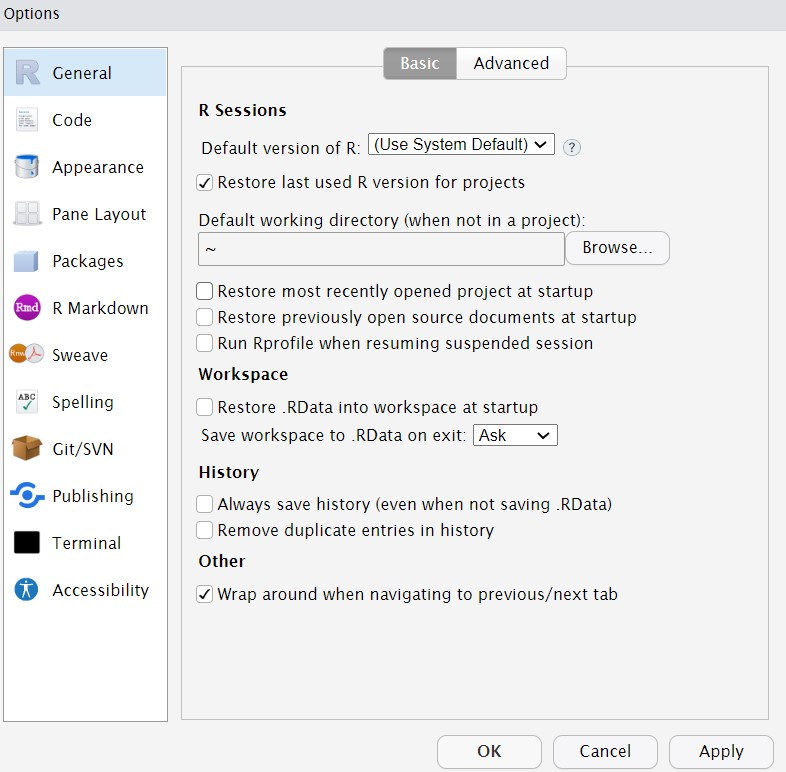
\includegraphics[width=1\linewidth]{images/global_options} 

}

\caption{Global options}\label{fig:img-options}
\end{figure}

\begin{itemize}
\item
  Dönem boyunca Rstudio kullanımına aşina olacaksınız. Bu süreci kolaylaştırmak için bağlantıları verilen dökümanlara göz atabilirsiniz.
\item
  \href{Kaynaklar/rstudio-ide.pdf}{Rstudio cheatsheet}
\item
  \href{Kaynaklar/rstudio_tutorial.pdf}{Oscar Torres* Reyna tutorial}
\end{itemize}

\hypertarget{hangi-r-suxfcruxfcmuxfcnuxfc-kullanmalux131sux131nux131z}{%
\section{Hangi R sürümünü kullanmalısınız?}\label{hangi-r-suxfcruxfcmuxfcnuxfc-kullanmalux131sux131nux131z}}

\begin{itemize}
\item
  R'yi bilgisayarınıza kurmanın avantajı, kullanmak için internete bağlı olmanız gerekmemesi, dosyalarınızı kaydetmenin ve yönetmenin daha kolay olması ve sunucunun çökmesi durumunda sorun yaşanmamasıdır (bu nadirdir, ancak olmuştur).
\item
  R sunucusunu kullanmanın avantajı, bilgisayraına herhangi bir şey yüklemenize gerek olmaması, sadece web tarayıcınız üzerinden erişebilmenizdir.
\item
  R'yi yükleyemeyeceğiniz bir bilgisayarınız varsa (örneğin Chromebook) veya R'yi bilgisayarınıza yüklemeyle ilgili ciddi sorunlarınız varsa sunucuyu kullanmanızı öneririz.
\end{itemize}

\hypertarget{r-studio-hakkux131nda}{%
\section{R Studio Hakkında}\label{r-studio-hakkux131nda}}

\begin{itemize}
\item
  R Studio, kodu deneyebileceğiniz bir konsola sahiptir (Şekil'de sol alt pencerede yer alır\ref{fig:img-rstudio}).
\item
  Ayrıca kod editörü (sol üst), ``Ortam'' sekmesinde oluşturduğunuz fonksiyonları ve nesneleri gösteren bir pencere ( sağ üst pencere) ve grafikleri, dosya paketlerini ve yardım belgelerini gösteren bir pencere ise (sağ alt) bulunur.
\end{itemize}

\begin{figure}

{\centering 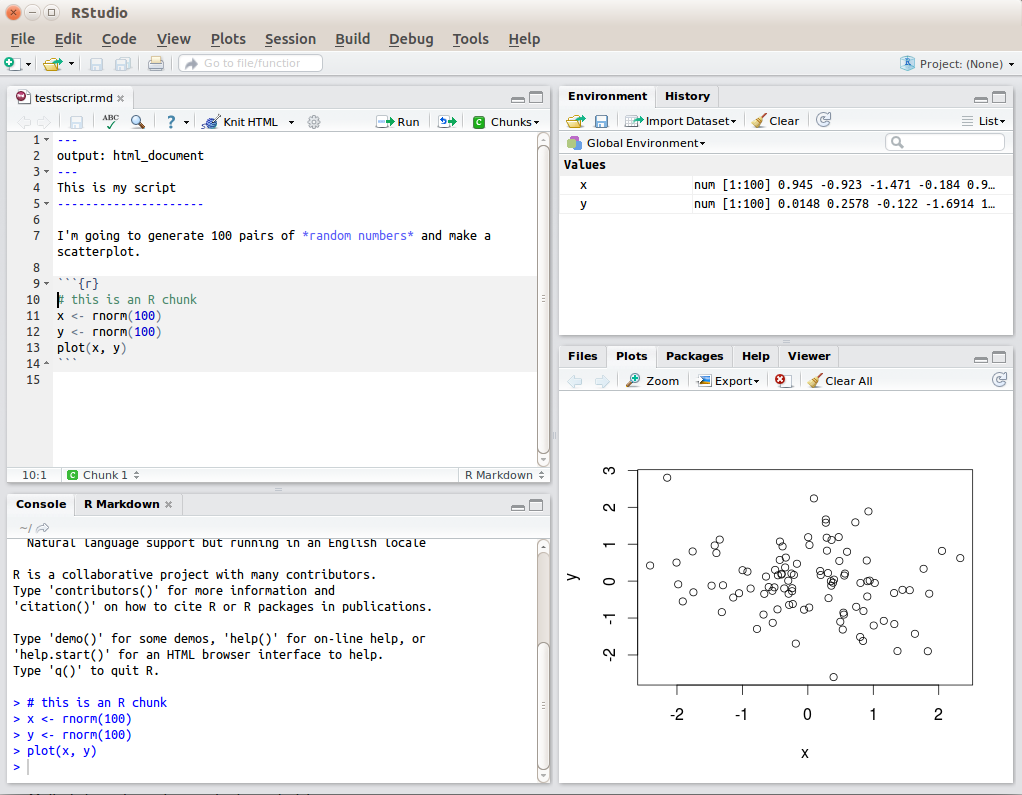
\includegraphics[width=1\linewidth]{images/Rstudio} 

}

\caption{RStudio arayüzü}\label{fig:img-rstudio}
\end{figure}

\begin{itemize}
\tightlist
\item
  Bu ders boyunca R Studio'da bulunan özelliklerin nasıl kullanılacağı hakkında daha fazla bilgi edineceksiniz, ancak R Studio ekibinden \href{https://rstudio.com/resources/webinars/programming-part-1-writing-code-in-rstudio/}{RStudio Essentials 1} izlemenizi şiddetle tavsiye ederim. Video yaklaşık 30 dakika sürmekte ve R Studio'nun ana bölümlerini tanıtmaktadır.
\end{itemize}

\hypertarget{r-temel-uxf6zellikler}{%
\section{R Temel Özellikler}\label{r-temel-uxf6zellikler}}

\begin{itemize}
\tightlist
\item
  R konsolda gorunen \textbf{\textgreater{}} isareti, R yaziliminin sizden komut bekledigini belirtir. R'in hesap makinesi olarak kullanim ornekleri sunulmustur.
\end{itemize}

\begin{Shaded}
\begin{Highlighting}[]
\DecValTok{2}\SpecialCharTok{+}\DecValTok{2}
\end{Highlighting}
\end{Shaded}

\begin{verbatim}
[1] 4
\end{verbatim}

\begin{itemize}
\tightlist
\item
  R boşluklara duyarlı değildir.
\end{itemize}

\begin{Shaded}
\begin{Highlighting}[]
\DecValTok{2}  \SpecialCharTok{+}       \DecValTok{2} 
\end{Highlighting}
\end{Shaded}

\begin{verbatim}
[1] 4
\end{verbatim}

\begin{Shaded}
\begin{Highlighting}[]
\DecValTok{2}\SpecialCharTok{+}
  \DecValTok{2}
\end{Highlighting}
\end{Shaded}

\begin{verbatim}
[1] 4
\end{verbatim}

\hypertarget{atama-operatoru}{%
\section{Atama Operatoru}\label{atama-operatoru}}

\begin{itemize}
\item
  Atama operatörü olarak ``küçüktür'' simgesi ile ``kısa çizgi'' simgesi \textbf{\texttt{\textless{}-}} simgeleri kullanılabilir.
\item
  \textbf{\texttt{\textless{}-}} yerine ``eşittir'' \textbf{\texttt{=}} simgesi de atama operatörü olarak kullanılabilir.
\item
  Ancak \textbf{\texttt{=}} operatörü programlama yaparken matematiksel eşitlikle karışabilmektedir.
\item
  Atama yapılacak nesne isimlendirilirken harflerle (A* Z veya a* z) başlamalıdır.
\item
  İsimlendirmeye harfle başlandıktan sonra rakamlar (0* 9), nokta (.) ve alt cizgi (\_) ile devam edilebilmektedir.
\item
  R harflerin küçük ve ya büyük olmasına karşı duyarlıdır.
\item
  R fonksiyonlarına benzer isimlerde nesne ismi kullanmamaya \textbf{dikkat edilmelidir.}
\item
  Ayrıca \textbf{c,C,D,F,I,q,t,T} gibi tek harfli nesne ismi kullanmaktan kaçınılmalıdır; bunların R'da özel anlamları bulunmaktadır.
\item
  R yazılımında \textbf{\#} işareti ile başlayan satir, yorum satırıdır.
\item
  Genellikle komutların anlamını açıklamak için kullanılmaktadır.
\item
  R, bu satırları dikkate almaz, bunlar sadece kullanıcılar için bilgi ve hatırlatıcı açıklamaları içermektedir.
\end{itemize}

\begin{Shaded}
\begin{Highlighting}[]
\CommentTok{\# Yorum satirlari kodlarinizi anlamli hale getirir.}
\NormalTok{a }\OtherTok{\textless{}{-}}  \DecValTok{2}
\NormalTok{y }\OtherTok{\textless{}{-}}\NormalTok{  a }\SpecialCharTok{*}\NormalTok{ a}
\NormalTok{y}
\end{Highlighting}
\end{Shaded}

\begin{verbatim}
[1] 4
\end{verbatim}

\hypertarget{basit-islemler}{%
\section{Basit İslemler}\label{basit-islemler}}

\begin{itemize}
\item
  toplama işlemi için \textbf{+},
\item
  çıkarma işlemi için \textbf{-},
\item
  çarpma işlemi için \textbf{*},
\item
  bölme işlemi için \textbf{/},
\item
  üs alma işlemi için \textbf{\^{}} veya *
\item
  mod alma icin ise \textbf{\%\%} operatorleri kullanılmaktadır.
\item
  Kodlamanızın büyük bir kısmı nesne oluşturmayı ve nesneleri manipüle etmeyi içerecektir. Nesneler bir şeyler içerir. Bu şeyler sayılar, kelimeler veya işlemlerin ve analizlerin sonucu olabilir
\end{itemize}

\textbf{Alıştırma Nesneler oluşturma}

\begin{itemize}
\tightlist
\item
  Aşağıdaki kodu kopyalayıp konsola yapıştırın, kodu kendi adınızı ve yaşınızı kullanacak şekilde değiştirin ve çalıştırın. Enviroment bölmesinde \texttt{ad}, \texttt{yas}, \texttt{gun}, \texttt{yeniyil} ve \texttt{veri} nesnelerinin göründüğünü göreceksiniz.
\end{itemize}

\begin{Shaded}
\begin{Highlighting}[]
\NormalTok{ad }\OtherTok{\textless{}{-}} \StringTok{"ada"}
\NormalTok{yas }\OtherTok{\textless{}{-}} \DecValTok{16} \SpecialCharTok{+} \DecValTok{20} 
\NormalTok{gun }\OtherTok{\textless{}{-}}\FunctionTok{Sys.Date}\NormalTok{()}
\NormalTok{yeniyil }\OtherTok{\textless{}{-}} \FunctionTok{as.Date}\NormalTok{(}\StringTok{"2024{-}01{-}01"}\NormalTok{)}
\NormalTok{veri }\OtherTok{\textless{}{-}} \FunctionTok{rnorm}\NormalTok{(}\AttributeTok{n =} \DecValTok{10}\NormalTok{, }\AttributeTok{mean =} \DecValTok{15}\NormalTok{, }\AttributeTok{sd =} \DecValTok{3}\NormalTok{)}
\end{Highlighting}
\end{Shaded}

\begin{figure}

{\centering 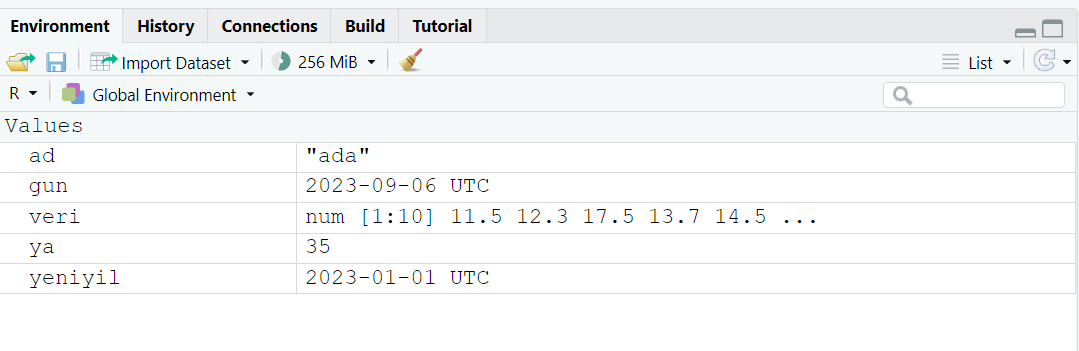
\includegraphics[width=1\linewidth]{images/objects-enviro} 

}

\caption{Calisma alanındaki nesneler}\label{fig:img-objects-enviro}
\end{figure}

\begin{itemize}
\item
  Bu örneklerde, \texttt{ad}, \texttt{yas} ve \texttt{yeniyil} her zaman \texttt{ada}, \texttt{36} değerlerini ve 2024 Yeni Yıl Günü tarihini içerecektir, ancak \texttt{gun} tarihi işletim sisteminden alacaktır ve \texttt{veri} rastgele oluşturulmuş bir veri kümesi olacaktır, bu nedenle bu nesnelerin değerleri statik olmayacaktır.
\item
  Daha da önemlisi, nesneler hesaplamalara dahil olabilir ve birbirleriyle etkileşime girebilir. Örneğin:
\end{itemize}

\begin{Shaded}
\begin{Highlighting}[]
\NormalTok{yas }\SpecialCharTok{+} \DecValTok{10}
\NormalTok{yeniyil }\SpecialCharTok{{-}}\NormalTok{ gun}
\FunctionTok{mean}\NormalTok{(veri)}
\end{Highlighting}
\end{Shaded}

\begin{verbatim}
[1] 46
Time difference of 105 days
[1] 14.8447
\end{verbatim}

\begin{itemize}
\tightlist
\item
  Son olarak, bu işlemlerin sonucunu yeni bir nesnede saklayabilirsiniz:
\end{itemize}

\begin{Shaded}
\begin{Highlighting}[]
\NormalTok{n1 }\OtherTok{\textless{}{-}}\NormalTok{ yas }\SpecialCharTok{+} \DecValTok{10}
\end{Highlighting}
\end{Shaded}

\begin{try}
\textless-\texttt{ifadesini}içerir\texttt{şeklinde\ okumak\ faydalı\ olabilir,\ örneğin}ad\texttt{ifadesi}ada`
metnini içerir.
\end{try}

\begin{itemize}
\tightlist
\item
  Bu ders boyunca sürekli olarak nesneler yaratacaksınız ve ilerledikçe onlar ve nasıl davrandıkları hakkında daha fazla bilgi edineceksiniz, ancak şimdilik bunların değerleri kaydetmenin bir yolu olduğunu, bu değerlerin sayı, metin veya işlemlerin sonucu olabileceğini ve yeni değişkenler oluşturmak için başka işlemlerde kullanılabileceğini anlamak yeterlidir.
\end{itemize}

\begin{info}
Nesnelerin `değişkenler' olarak adlandırıldığını da görebilirsiniz.
Programlama terimlerinde ikisi arasında fark vardır, ancak çok sık
eşanlamlı olarak kullanılırlar.
\end{info}

\textbf{Alıştırma Nesneler oluşturma}

\begin{itemize}
\tightlist
\item
  Aşağıdaki kodu kopyalayıp konsola yapıştırın.
\item
  Eni 4 cm, boyu 10 cm bir dikdörtgenin alanı hesaplayınız.
\end{itemize}

\begin{Shaded}
\begin{Highlighting}[]
\CommentTok{\# en nesnesi tanimlama}

\CommentTok{\# boy nesnesi tanimlama}

\CommentTok{\# alan nesnesi tanimlama}

\CommentTok{\# alan nesnesini yazdirma}
\end{Highlighting}
\end{Shaded}

\begin{verbatim}
[1] 40
\end{verbatim}

\begin{itemize}
\tightlist
\item
  Eni 4 cm, boyu 10 cm bir dikdörtgenin köşegen uzunluğunu hesaplayınız.
\end{itemize}

\begin{Shaded}
\begin{Highlighting}[]
\CommentTok{\# en nesnesi tanimlama}

\CommentTok{\# boy nesnesi tanimlama}

\CommentTok{\# kosegen nesnesi tanimlama}

\CommentTok{\# kosegen nesnesini yazdirma}
\end{Highlighting}
\end{Shaded}

\begin{verbatim}
[1] 10.77033
\end{verbatim}

\hypertarget{uxf6dev}{%
\subsection{Ödev}\label{uxf6dev}}

Datacamp hesapınızda yer alan 🔗\href{https://app.datacamp.com/workspace/w/27893d74-f669-4ea4-964d-d8c367b6345e/edit}{01\_Temeller workspaceni} tamamlayınız.

\hypertarget{r-paketler}{%
\chapter{R Paketler}\label{r-paketler}}

\begin{itemize}
\item
  R'yi yüklediğinizde, veri işleme ve istatistiksel analiz seçenekleri de dahil olmak üzere bir dizi fonksiyona erişebilirsiniz. Varsayılan kurulumda yer alan fonksiyonlar genellikle \textbf{Temel R/Base R} olarak adlandırılır ve birçok Temel R fonksiyonunu gösteren faydalı bir cheatsheet sayfası vardır 🔗\href{https://github.com/rstudio/cheatsheets/raw/main/base-r.pdf}{cheatsheet}
\item
  \textbf{Temel R} telefonunuzda gelen varsayılan uygulamalar, paketleri ise ayrıca indirmeniz gereken ek uygulamalar olarak düşünmek faydalı olabilir.
\item
  R fonksiyonları \textbf{ayrı paketler} halinde düzenlenmişlerdir. Böylece gerekli paketlerle çalışarak daha az bellek kullanımı ve hızlı işlem gücü sağlanır.
\item
  Bu paketlerin bir başka avantajı da yazılan fonksiyonlardan oluşan paketlerin CRAN'den temin edilerek yüklenebilmesidir.
\item
  Her paketin bir yaratıcısı ve kendisine ait bir yardım dosyası bulunur.
\end{itemize}

\begin{Shaded}
\begin{Highlighting}[]
\CommentTok{\# paket yukleme}
\FunctionTok{install.packages}\NormalTok{(}\StringTok{"CTT"}\NormalTok{)}
\CommentTok{\# paket aktive etme}
\FunctionTok{library}\NormalTok{(CTT)}
\end{Highlighting}
\end{Shaded}

\begin{itemize}
\item
  Paket yükleme işlemi Rstudio'da yer alan menüler aracılığı ile de yapılabilmektedir.
\item
  R paketleri R fonksiyonlarının, verilerinin ve iyi derlenmiş bir formatta kodların kombinasyonlarından oluşmaktadır. \texttt{library()} komutu ile kişisel kütüphanenizdeki yüklü paketleri görebilirsiniz.
\item
  Sadece temel pakette 1000'den fazla fonksiyon bulunmaktadır.
\end{itemize}

\begin{Shaded}
\begin{Highlighting}[]
\CommentTok{\# temel paket fonksiyonlarina ulasimak icin  }
\NormalTok{fonksiyonlar }\OtherTok{\textless{}{-}}  \FunctionTok{builtins}\NormalTok{()}
\FunctionTok{length}\NormalTok{(fonksiyonlar)}
\end{Highlighting}
\end{Shaded}

\begin{verbatim}
## [1] 1380
\end{verbatim}

\begin{Shaded}
\begin{Highlighting}[]
\NormalTok{fonksiyonlar[}\DecValTok{910}\SpecialCharTok{:}\DecValTok{920}\NormalTok{]}
\end{Highlighting}
\end{Shaded}

\begin{verbatim}
##  [1] "Cstack_info"                "crossprod"                 
##  [3] "cospi"                      "cosh"                      
##  [5] "cos"                        "contributors"              
##  [7] "Conj"                       "conflicts"                 
##  [9] "conflictRules"              "conditionMessage.condition"
## [11] "conditionMessage"
\end{verbatim}

\begin{figure}
\centering
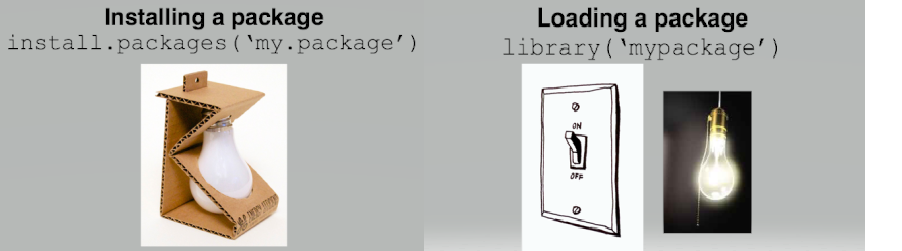
\includegraphics[width=0.7\textwidth,height=\textheight]{images/packagebulb.png}
\caption{yükle-etkinleştir}
\end{figure}

\hypertarget{alux131ux15ftux131rma-tidyverse-yuxfckleme}{%
\subsection{Alıştırma : tidyverse yükleme}\label{alux131ux15ftux131rma-tidyverse-yuxfckleme}}

\begin{itemize}
\tightlist
\item
  Bir paketi kullanabilmek için önce onu yüklemeniz gerekir. Aşağıdaki kod, bu derste çok sık kullanacağımız bir paket olan \texttt{tidyverse} paketini yükler.
\end{itemize}

\begin{Shaded}
\begin{Highlighting}[]
\FunctionTok{install.packages}\NormalTok{(}\StringTok{"tidyverse"}\NormalTok{)}
\end{Highlighting}
\end{Shaded}

\begin{itemize}
\tightlist
\item
  Bir paketi yalnızca bir kez yüklemeniz gerekir, ancak R'yi her başlattığınızda kullanmak istediğiniz paketleri yüklemeniz gerekir, benzer şekilde telefonunuza bir uygulamayı bir kez yüklemeniz gerekir, ancak her kullanmak istediğinizde açmanız gerekir.
\end{itemize}

\begin{info}
\textbf{UYARI: WARNING: Rtools is required to build R packages'' gibi
bir hata mesajı alırsanız, {[}Rtools{]}
(https://cran.r-project.org/bin/windows/Rtools/) adlı ekstra bir yazılım
indirmeniz ve yüklemeniz gerekebilir.}
\end{info}

\hypertarget{alux131ux15ftux131rma-tidyverse-etkinleux15ftir}{%
\subsection{Alıştırma : tidyverse etkinleştir}\label{alux131ux15ftux131rma-tidyverse-etkinleux15ftir}}

\begin{itemize}
\tightlist
\item
  Tidyverse'i etkinleştirmek için aşağıdaki kodu çalıştırın.
\end{itemize}

\begin{Shaded}
\begin{Highlighting}[]
\FunctionTok{library}\NormalTok{(tidyverse)}
\end{Highlighting}
\end{Shaded}

\begin{itemize}
\item
  Bir hata mesajı gibi görünen bir şey alacaksınız - öyle değil. Bu sadece R'nin size ne yaptığını anlatmasıdır.
\item
  Şimdi \texttt{tidyverse} paketini etkinleştirdiğimize göre, içerdiği fonksiyonlardan herhangi birini kullanabiliriz, ancak unutmayın, R'yi her başlattığınızda \texttt{library()} fonksiyonunu çalıştırmanız gerekir.
\end{itemize}

\hypertarget{yardux131m-sayfalarux131}{%
\section{Yardım Sayfaları}\label{yardux131m-sayfalarux131}}

\begin{itemize}
\tightlist
\item
  R'da temel ve diğer paketlerde yer alan fonksiyonların işlevleri görmek için yardım sayfalarını inceleyebilirsiniz. \texttt{?} ve \texttt{help()} fonksiyonları ayni işleve sahiptir.
\end{itemize}

\begin{Shaded}
\begin{Highlighting}[]
\NormalTok{?is.na}

\FunctionTok{help}\NormalTok{(sqrt)}
\end{Highlighting}
\end{Shaded}

\begin{itemize}
\tightlist
\item
  Örneğin CTT paketini hem yüklediniz hem de etkinleştirdiniz. Paket fonksiyon ve veri içeriğini aşağıdaki komutlarla görebilirsiniz.
\end{itemize}

\begin{Shaded}
\begin{Highlighting}[]
\CommentTok{\# install.packages(CTT)}
\FunctionTok{library}\NormalTok{(CTT)}
\FunctionTok{ls}\NormalTok{(}\StringTok{"package:CTT"}\NormalTok{) }
\FunctionTok{data}\NormalTok{(}\AttributeTok{package =} \StringTok{"CTT"}\NormalTok{) }\CommentTok{\# yeni bir sekmede acilir.}
\NormalTok{?reliability}
\end{Highlighting}
\end{Shaded}

\begin{itemize}
\tightlist
\item
  Etkinleştirdiğiniz paketlerde yer alan fonksiyonların yardım sayfalarına ulaşabilirsiniz.
\end{itemize}

\hypertarget{conflicts}{%
\section{Paket çakışmaları}\label{conflicts}}

\begin{itemize}
\tightlist
\item
  Daha da fazla fonksiyona sahip binlerce farklı R paketi vardır. Ne yazık ki, bazen farklı paketler aynı fonksiyon isimlerine sahiptir. Örneğin, \texttt{dplyr} ve \texttt{MASS} paketlerinin her ikisi de \texttt{select()} adında bir fonksiyona sahiptir. Bu paketlerin her ikisini de yüklerseniz, R size bir çakışma olduğunu söyleyen bir uyarı üretecektir.
\end{itemize}

\begin{Shaded}
\begin{Highlighting}[]
\FunctionTok{library}\NormalTok{(dplyr)}
\FunctionTok{library}\NormalTok{(MASS)}
\end{Highlighting}
\end{Shaded}

\begin{verbatim}
## 
## Attaching package: 'MASS'
\end{verbatim}

\begin{verbatim}
## The following object is masked from 'package:dplyr':
## 
##     select
\end{verbatim}

\begin{itemize}
\item
  Bu durumda, R size \texttt{dplyr} paketindeki \texttt{select()} fonksiyonunun aynı isimli başka bir fonksiyon tarafından gizlendiğini (veya `maskelendiğini') söylüyor. Eğer \texttt{select()} fonksiyonunu kullanmayı deneseydiniz, R en son yüklenen paketteki fonksiyonu kullanacaktı - bu durumda \texttt{MASS} fonksiyonunu kullanacaktı.
\item
  Belirli bir fonksiyon için hangi paketi kullanmak istediğinizi belirtmek istiyorsanız, örneğin \texttt{package::function} biçiminde kod kullanabilirsiniz:
\end{itemize}

\begin{Shaded}
\begin{Highlighting}[]
\NormalTok{dplyr}\SpecialCharTok{::}\FunctionTok{select}\NormalTok{()}
\NormalTok{MASS}\SpecialCharTok{::}\FunctionTok{select}\NormalTok{()}
\end{Highlighting}
\end{Shaded}

\hypertarget{paket-guxfcncelleme}{%
\section{Paket Güncelleme}\label{paket-guxfcncelleme}}

\begin{itemize}
\item
  R ve R Studio güncellemelerine ek olarak, paketlerin yazarları da bazen kodlarını günceller. Bu, bir pakete fonksiyon eklemek için olabileceği gibi hataları düzeltmek için de olabilir. \textbf{Kaçınılması gereken bir şey, yüklü bir paketi istemeden güncellemektir.}
\item
  \texttt{install.packages()} fonksiyonunu çalıştırdığınızda, her zaman paketin en son sürümü yüklenir ve yüklemiş olabileceğiniz eski sürümlerin üzerine yazılır. Bazen bu bir sorun teşkil etmez, ancak bazen paket önemli ölçüde değiştiği için güncellemenin kodunuzun artık çalışmadığı anlamına geldiğini görürsünüz. Bir paketin eski bir sürümüne geri dönmek mümkündür ancak yine de bundan kaçınmaya çalışın.
\end{itemize}

\begin{info}
Bir paketin üzerine yanlışlıkla daha sonraki bir sürümün yazılmasını
önlemek için, sizin veya bir başkasının kodu yanlışlıkla çalıştırması
ihtimaline karşı analiz komut dosyalarınıza \texttt{install.packages()}
i \textbf{asla} dahil etmemelisiniz.
\end{info}

\hypertarget{r-ve-rstudioya-nasux131l-alux131ntux131-yapux131lux131r}{%
\section{R ve RStudio'ya nasıl alıntı yapılır}\label{r-ve-rstudioya-nasux131l-alux131ntux131-yapux131lux131r}}

\begin{itemize}
\item
  R'a atıfta bulunmanız ve referans vermeniz gereken bilimsel bir rapor yazmaktan biraz uzak olabilirsiniz, ancak zamanı geldiğinde bunu onu geliştiren insanlara (çoğu ücretsiz!) kredi vermek için yapmak önemlidir. R, RStudio ve kullandığınız paketler için ayrı alıntılar sağlamalısınız.
\item
  Kullandığınız R sürümü için atıf almak için, size her zaman en son atıfı sağlayacak olan \texttt{citation()} fonksiyonunu çalıştırmanız yeterlidir.
\end{itemize}

\begin{Shaded}
\begin{Highlighting}[]
\FunctionTok{citation}\NormalTok{()}
\end{Highlighting}
\end{Shaded}

\begin{verbatim}
## 
## To cite R in publications use:
## 
##   R Core Team (2022). R: A language and environment for statistical
##   computing. R Foundation for Statistical Computing, Vienna, Austria.
##   URL https://www.R-project.org/.
## 
## A BibTeX entry for LaTeX users is
## 
##   @Manual{,
##     title = {R: A Language and Environment for Statistical Computing},
##     author = {{R Core Team}},
##     organization = {R Foundation for Statistical Computing},
##     address = {Vienna, Austria},
##     year = {2022},
##     url = {https://www.R-project.org/},
##   }
## 
## We have invested a lot of time and effort in creating R, please cite it
## when using it for data analysis. See also 'citation("pkgname")' for
## citing R packages.
\end{verbatim}

\begin{itemize}
\tightlist
\item
  Kullandığınız herhangi bir paket için atıf oluşturmak için, atıf yapmak istediğiniz paketin adıyla birlikte \texttt{citation()} işlevini de kullanabilirsiniz.
\end{itemize}

\begin{Shaded}
\begin{Highlighting}[]
\FunctionTok{citation}\NormalTok{(}\StringTok{"tidyverse"}\NormalTok{)}
\end{Highlighting}
\end{Shaded}

\begin{verbatim}
## 
## To cite package 'tidyverse' in publications use:
## 
##   Wickham H, Averick M, Bryan J, Chang W, McGowan LD, François R,
##   Grolemund G, Hayes A, Henry L, Hester J, Kuhn M, Pedersen TL, Miller
##   E, Bache SM, Müller K, Ooms J, Robinson D, Seidel DP, Spinu V,
##   Takahashi K, Vaughan D, Wilke C, Woo K, Yutani H (2019). "Welcome to
##   the tidyverse." _Journal of Open Source Software_, *4*(43), 1686.
##   doi:10.21105/joss.01686 <https://doi.org/10.21105/joss.01686>.
## 
## A BibTeX entry for LaTeX users is
## 
##   @Article{,
##     title = {Welcome to the {tidyverse}},
##     author = {Hadley Wickham and Mara Averick and Jennifer Bryan and Winston Chang and Lucy D'Agostino McGowan and Romain François and Garrett Grolemund and Alex Hayes and Lionel Henry and Jim Hester and Max Kuhn and Thomas Lin Pedersen and Evan Miller and Stephan Milton Bache and Kirill Müller and Jeroen Ooms and David Robinson and Dana Paige Seidel and Vitalie Spinu and Kohske Takahashi and Davis Vaughan and Claus Wilke and Kara Woo and Hiroaki Yutani},
##     year = {2019},
##     journal = {Journal of Open Source Software},
##     volume = {4},
##     number = {43},
##     pages = {1686},
##     doi = {10.21105/joss.01686},
##   }
\end{verbatim}

\begin{itemize}
\tightlist
\item
  Kullandığınız RStudio sürümüne ait alıntıyı oluşturmak için \texttt{RStudio.Vesion()} fonksiyonunu kullanabilirsiniz:
\end{itemize}

\begin{Shaded}
\begin{Highlighting}[]
\FunctionTok{RStudio.Version}\NormalTok{()}
\end{Highlighting}
\end{Shaded}

\begin{itemize}
\tightlist
\item
  Son olarak, yöntem bölümünüzün yazımında bunun nasıl görünebileceğine dair bir örnek:
\end{itemize}

\begin{quote}
Analiz R (R Core Team, 2020), RStudio (Rstudio Team, 2020) ve tidyverse paketi (Wickham, 2017) kullanılarak gerçekleştirilmiştir.
\end{quote}

\begin{itemize}
\tightlist
\item
  Belirtildiği gibi, bunu bir süre yapmak zorunda kalmayabilirsiniz, ancak yaptığınızda buna geri dönün çünkü açık kaynak topluluğuna çalışmaları için kredi vermek önemlidir.
\end{itemize}

\hypertarget{fonksiyonlar}{%
\chapter{Fonksiyonlar}\label{fonksiyonlar}}

\begin{itemize}
\item
  Fonksiyon belli bir görevi yerine getirmek için yazılan bir grup komuttur.
\item
  Fonksiyonların çalışması için girdilerinin olması gerekmektedir. Fonksiyonlar girdileri ile yaptıkları işlem sonucunda bir çıktı oluştururlar.
\item
  Fonksiyonlar girdileri o fonksiyonun çalışması için önceden belirlenen \textbf{argümanlar} ve o argümanların değerlerinden oluşur. (dilbilimle ilgileniyorsanız, bunları bir özne ve nesne gerektiren fiiller olarak düşünmek isteyebilirsiniz)
\item
  Fonksiyonların kullanımında üç noktaya dikkat edilmelidir.

  \begin{enumerate}
  \def\labelenumi{\arabic{enumi}.}
  \tightlist
  \item
    argümanların sırası
  \item
    argümanların olağan (default) değerleri
  \item
    bazı argümanların zorunlu, bazı argümanların opsiyonel olmasıdır
  \end{enumerate}
\item
  Bir fonksiyonun aldığı tüm argümanlara yardım dokümantasyonunu kullanarak \texttt{?function} formatını kullanarak bakabilirsiniz. Bazı argümanlar zorunlu, bazıları ise isteğe bağlıdır. İsteğe bağlı bağımsız değişkenler, herhangi bir değer girmezseniz genellikle varsayılan/olağan (normalde yardım belgelerinde belirtilen) bir değer kullanır.
\item
  Örnek olarak, normal dağılıma sahip bir sayı kümesini rastgele üreten \texttt{rnorm()} fonksiyonunun yardım belgelerine bakalım.
\item
  Bir fonksiyonun aldığı tüm argümanlara yardım dokümantasyonunu kullanarak \texttt{?function} formatını kullanarak bakabilirsiniz. Bazı argümanlar zorunlu, bazıları ise isteğe bağlıdır. İsteğe bağlı bağımsız değişkenler, herhangi bir değer girmezseniz genellikle varsayılan/olağan (normalde yardım belgelerinde belirtilen) bir değer kullanır.
\end{itemize}

\textbf{Alıştırma }

\begin{itemize}
\tightlist
\item
  R Studio'yu açın ve konsola aşağıdaki kodu yazın:
\end{itemize}

\begin{Shaded}
\begin{Highlighting}[]
\NormalTok{?rnorm}
\end{Highlighting}
\end{Shaded}

\begin{itemize}
\tightlist
\item
  \texttt{rnorm()} için yardım belgeleri sağ alt yardım panelinde görünmelidir. Kullanım bölümünde, \texttt{rnorm()}un aşağıdaki formu aldığını görüyoruz:
\end{itemize}

\begin{Shaded}
\begin{Highlighting}[]
\FunctionTok{rnorm}\NormalTok{(n, }\AttributeTok{mean =} \DecValTok{0}\NormalTok{, }\AttributeTok{sd =} \DecValTok{1}\NormalTok{)}
\end{Highlighting}
\end{Shaded}

\begin{itemize}
\item
  Argümanlar bölümünde, her bir argüman için açıklamalar bulunmaktadır. \texttt{n} oluşturmak istediğimiz gözlem sayısı, \texttt{mean} oluşturacağımız veri noktalarının ortalaması ve \texttt{sd} verinin standart sapmasıdır. Ayrıntılar bölümünde, \texttt{mean} ve \texttt{sd} için herhangi bir değer girilmezse, bu değerler için varsayılan olarak 0 ve 1 kullanılacağı belirtilir. \texttt{n} için varsayılan bir değer olmadığından, belirtilmesi gerekir, aksi takdirde kod çalışmaz.
\item
  Bir örnek deneyelim ve R'den 5 rastgele sayı üretmesini istemek için gerekli \texttt{n} argümanını değiştirelim.
\end{itemize}

\textbf{Alıştırma II}

\begin{itemize}
\tightlist
\item
  Aşağıdaki kodu kopyalayıp konsola yapıştırın.
\end{itemize}

\begin{Shaded}
\begin{Highlighting}[]
\FunctionTok{set.seed}\NormalTok{(}\DecValTok{12042016}\NormalTok{)}
\FunctionTok{rnorm}\NormalTok{(}\AttributeTok{n =} \DecValTok{5}\NormalTok{)}
\end{Highlighting}
\end{Shaded}

\begin{verbatim}
## [1] -0.2896163 -0.6428964  0.5829221 -0.3286728 -0.5110101
\end{verbatim}

\begin{itemize}
\tightlist
\item
  Bu sayıların ortalaması 0 ve SD'si 1'dir. Şimdi farklı bir sayı kümesi üretmek için ek argümanları değiştirebiliriz.
\end{itemize}

\begin{Shaded}
\begin{Highlighting}[]
\FunctionTok{rnorm}\NormalTok{(}\AttributeTok{n =} \DecValTok{5}\NormalTok{, }\AttributeTok{mean =} \DecValTok{10}\NormalTok{, }\AttributeTok{sd =} \DecValTok{2}\NormalTok{)}
\end{Highlighting}
\end{Shaded}

\begin{verbatim}
## [1] 13.320853  9.377956 10.235461  9.811793 13.019102
\end{verbatim}

\begin{itemize}
\tightlist
\item
  Bu kez R yine 5 rastgele sayı üretti, ancak şimdi bu sayı kümesi belirtildiği gibi 10 ortalama ve 2 sd değerine sahip. Bir fonksiyonun hangi argümanları gerektirdiğini anlamanıza yardımcı olması için yardım belgelerini kullanmayı her zaman unutmayın.
\end{itemize}

\begin{info}
Eğer internette kod örneklerine bakıyorsanız, sık sık
\texttt{set.seed()} fonksiyonu ile başlayan kodlar görebilirsiniz. Bu
fonksiyon rastgele sayı üretecini kontrol eder - rastgele sayı üreten
herhangi bir fonksiyon kullanıyorsanız (\texttt{rnorm()} gibi),
\texttt{set.seed()} fonksiyonunu çalıştırmak aynı sonucu almanızı
sağlayacaktır (bazı durumlarda yapmak istediğiniz şey bu olmayabilir).
Bu örnekte \texttt{set.seed()} diyoruz, bu aynı rastgele sayıları
alacağınız anlamına geliyor.
\end{info}

\hypertarget{arguxfcman-isimleri}{%
\section{Argüman isimleri}\label{arguxfcman-isimleri}}

\begin{itemize}
\tightlist
\item
  Yukarıdaki örneklerde, kodumuzdaki bağımsız değişken adlarını yazdık (örneğin, \texttt{n}, \texttt{mean}, \texttt{sd}), ancak bu kesinlikle gerekli değildir. Aşağıdaki iki kod satırının her ikisi de aynı sonucu üretecektir (\texttt{rnorm()} fonksiyonunu her çalıştırdığınızda rastgele olduğu için biraz farklı bir sayı kümesi üretecektir, ancak yine de aynı ortalama ve SD'ye sahip olacaklardır):
\end{itemize}

\begin{Shaded}
\begin{Highlighting}[]
\FunctionTok{rnorm}\NormalTok{(}\AttributeTok{n =} \DecValTok{6}\NormalTok{, }\AttributeTok{mean =} \DecValTok{3}\NormalTok{, }\AttributeTok{sd =} \DecValTok{1}\NormalTok{)}
\FunctionTok{rnorm}\NormalTok{(}\DecValTok{6}\NormalTok{, }\DecValTok{3}\NormalTok{, }\DecValTok{1}\NormalTok{)}
\end{Highlighting}
\end{Shaded}

\begin{itemize}
\item
  Önemli olarak, eğer argüman isimlerini yazmazsanız, R argümanların varsayılan sırasını kullanacaktır, yani \texttt{rnorm} için girdiğiniz ilk sayının \texttt{n} olduğunu varsayacaktır. ikinci sayı \texttt{mean} ve üçüncü sayı \texttt{sd}dir.
\item
  Eğer argüman isimlerini yazarsanız, argümanları istediğiniz sırada yazabilirsiniz:
\end{itemize}

\begin{Shaded}
\begin{Highlighting}[]
\FunctionTok{rnorm}\NormalTok{(}\AttributeTok{sd =} \DecValTok{1}\NormalTok{, }\AttributeTok{n =} \DecValTok{6}\NormalTok{, }\AttributeTok{mean =} \DecValTok{3}\NormalTok{)}
\end{Highlighting}
\end{Shaded}

\begin{itemize}
\item
  R'yi ilk öğrenirken, fonksiyonun her bir parçasının ne yaptığını hatırlamanıza ve anlamanıza yardımcı olabileceğinden, argüman adlarını yazmayı yararlı bulabilirsiniz. Ancak, becerileriniz ilerledikçe argüman adlarını atlamayı daha hızlı bulabilirsiniz ve ayrıca argüman adlarını kullanmayan çevrimiçi kod örnekleri göreceksiniz, bu nedenle her bir kod parçasının hangi argümana atıfta bulunduğunu anlayabilmek önemlidir (veya kontrol etmek için yardım belgelerine bakın).
\item
  Bu derste, her bir fonksiyonu ilk kez kullandığımızda argüman adlarını her zaman yazacağız, ancak sonraki kullanımlarda bunlar atlanabilir.
\end{itemize}

\hypertarget{tab-ile-otomatik-tamamlama}{%
\section{TAB ile otomatik tamamlama}\label{tab-ile-otomatik-tamamlama}}

\begin{itemize}
\tightlist
\item
  R Studio'nun çok kullanışlı bir özelliği, fonksiyonlar için TAB otomatik tamamlama özelliğidir (bkz. Şekil \ref{fig:img-autocomplete}). Fonksiyonun adını yazıp tab tuşuna basarsanız, R Studio size fonksiyonun aldığı argümanları kısa bir açıklama ile birlikte gösterecektir. Argüman adının üzerinde enter tuşuna basarsanız, tıpkı telefonunuzdaki otomatik tamamlama gibi adı sizin için dolduracaktır. Bu, R'yi ilk öğrenirken inanılmaz derecede kullanışlıdır ve bu özelliği sık sık kullanmayı \textbf{unutmamalısınız.}
\end{itemize}

\begin{figure}

{\centering 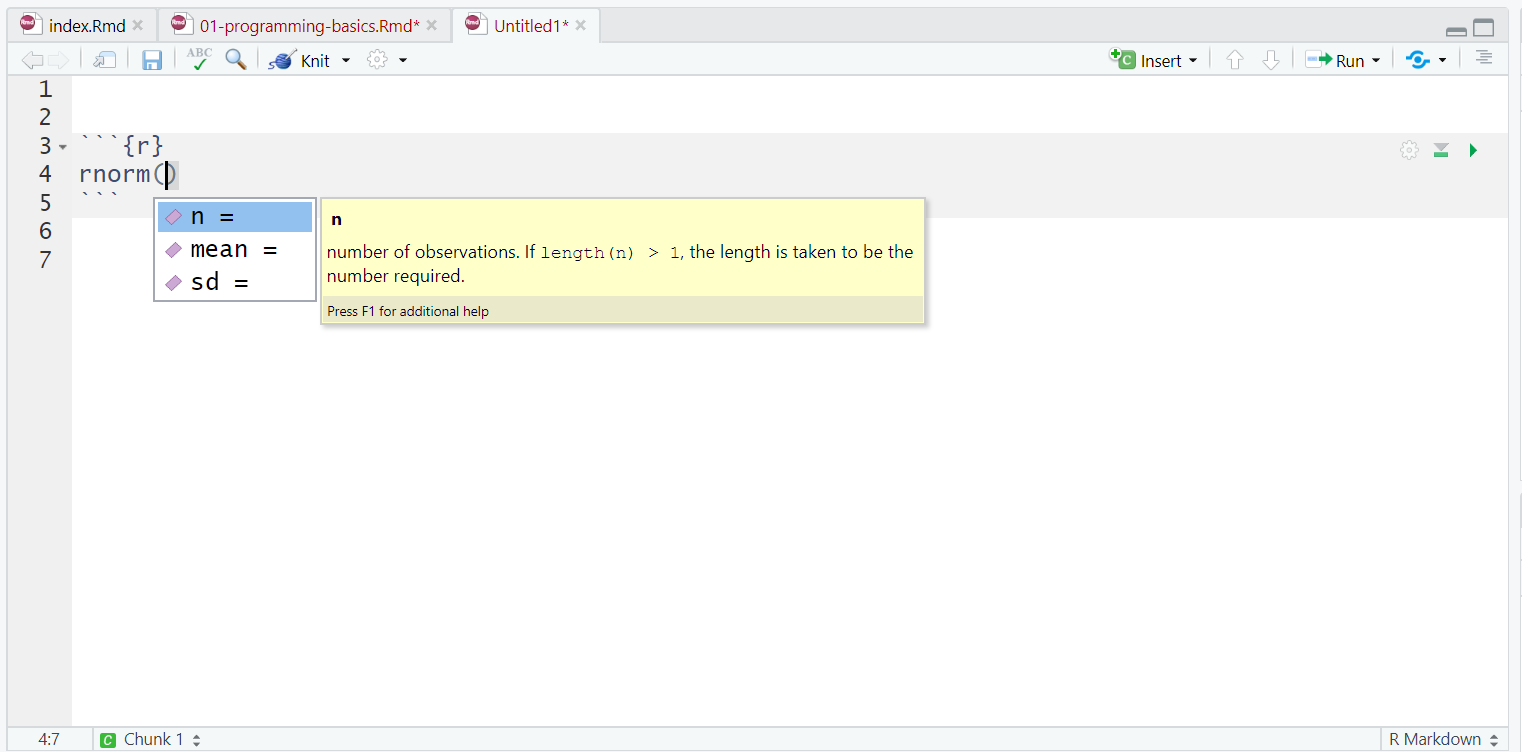
\includegraphics[width=1\linewidth]{images/autocomplete} 

}

\caption{Tab ile otomatik durdurma}\label{fig:img-autocomplete}
\end{figure}

\hypertarget{kiux15fisel-tanux131mlux131-fonksiyon}{%
\section{Kişisel tanımlı fonksiyon}\label{kiux15fisel-tanux131mlux131-fonksiyon}}

\begin{itemize}
\tightlist
\item
  Kişisel tanımlı fonksiyon yazılması şablonu aşağıdaki gibidir.
\end{itemize}

\begin{Shaded}
\begin{Highlighting}[]
\NormalTok{fonksiyonadi}\OtherTok{\textless{}{-}}  \ControlFlowTok{function}\NormalTok{(argumanlar ve olagan degerleri)\{}
\NormalTok{  kodlar}
  \FunctionTok{return}\NormalTok{()}
\NormalTok{\}}
\end{Highlighting}
\end{Shaded}

\begin{itemize}
\tightlist
\item
  Oluşturulan fonksiyon çalıştırılırken ise aşağıdaki şeklinde çalıştırılır.
\end{itemize}

\begin{Shaded}
\begin{Highlighting}[]
\FunctionTok{fonksiyonadi}\NormalTok{(argumanlar ve degerleri)}
\end{Highlighting}
\end{Shaded}

\begin{itemize}
\tightlist
\item
  Kare alma işlemi aşağıdaki şekilde yapılabilir.
\end{itemize}

\begin{Shaded}
\begin{Highlighting}[]
\NormalTok{sayi }\OtherTok{\textless{}{-}}  \DecValTok{4}
\NormalTok{sayi }\SpecialCharTok{*}\NormalTok{ sayi}
\NormalTok{sayi }\SpecialCharTok{\^{}}\DecValTok{2}
\end{Highlighting}
\end{Shaded}

\begin{verbatim}
## [1] 16
## [1] 16
\end{verbatim}

\begin{itemize}
\tightlist
\item
  Bu işlem sürekli yapılacaksa fonksiyon olarak yazılabilir.
\end{itemize}

\begin{Shaded}
\begin{Highlighting}[]
\CommentTok{\# kare alma fonksiyonu}
\NormalTok{kare\_al }\OtherTok{\textless{}{-}}  \ControlFlowTok{function}\NormalTok{(sayi)\{}
  \FunctionTok{return}\NormalTok{(sayi}\SpecialCharTok{*}\NormalTok{sayi)}
\NormalTok{  \}}
\FunctionTok{kare\_al}\NormalTok{(}\DecValTok{4}\NormalTok{)}
\end{Highlighting}
\end{Shaded}

\begin{verbatim}
## [1] 16
\end{verbatim}

\begin{itemize}
\tightlist
\item
  Farklı dereceden üsler alabilen bir fonksiyon yazalım.
\end{itemize}

\begin{Shaded}
\begin{Highlighting}[]
\CommentTok{\#üs alma}
\NormalTok{üs\_al}\OtherTok{\textless{}{-}}  \ControlFlowTok{function}\NormalTok{(x,us)\{}
  \FunctionTok{return}\NormalTok{(x}\SpecialCharTok{\^{}}\NormalTok{us)}
\NormalTok{  \}}
\NormalTok{ü}\FunctionTok{s\_al}\NormalTok{(}\DecValTok{3}\NormalTok{,}\DecValTok{4}\NormalTok{)}
\end{Highlighting}
\end{Shaded}

\begin{verbatim}
## [1] 81
\end{verbatim}

\begin{itemize}
\tightlist
\item
  Argümanlardan birine olağan değer girilmesi
\end{itemize}

\begin{Shaded}
\begin{Highlighting}[]
\CommentTok{\#üs alma}
\NormalTok{üs\_al}\OtherTok{\textless{}{-}}  \ControlFlowTok{function}\NormalTok{(x,}\AttributeTok{us=}\DecValTok{2}\NormalTok{)\{}
  \FunctionTok{return}\NormalTok{(x}\SpecialCharTok{\^{}}\NormalTok{us)}
\NormalTok{  \}}
\NormalTok{ü}\FunctionTok{s\_al}\NormalTok{(}\DecValTok{3}\NormalTok{) }\CommentTok{\# us argumanin olagan degeri olan}
\CommentTok{\# 2 olduğu için argumana }
\CommentTok{\# deger girilmediginde kare alir.}
\end{Highlighting}
\end{Shaded}

\begin{verbatim}
## [1] 9
\end{verbatim}

\begin{itemize}
\tightlist
\item
  Aşağıdaki fonksiyona 3 ve 4 değerleri girilirse çıktı ne olur?
\end{itemize}

\begin{Shaded}
\begin{Highlighting}[]
\NormalTok{myfunc }\OtherTok{\textless{}{-}}  \ControlFlowTok{function}\NormalTok{(x,y)}
\NormalTok{\{}
\NormalTok{a }\OtherTok{\textless{}{-}}\NormalTok{  x}\SpecialCharTok{+}\NormalTok{y}
\NormalTok{b }\OtherTok{\textless{}{-}}\NormalTok{  x}\SpecialCharTok{*}\NormalTok{ y}
\FunctionTok{return}\NormalTok{(a}\SpecialCharTok{*}\NormalTok{b)}
\NormalTok{\}}
\FunctionTok{myfunc}\NormalTok{(}\DecValTok{3}\NormalTok{,}\DecValTok{4}\NormalTok{)}
\end{Highlighting}
\end{Shaded}

\begin{itemize}
\tightlist
\item
  \texttt{mean()} fonksiyonu en sık kullandığımız fonksiyonlardan biridir.
\end{itemize}

\begin{Shaded}
\begin{Highlighting}[]
\NormalTok{x }\OtherTok{\textless{}{-}}  \FunctionTok{c}\NormalTok{(}\DecValTok{1}\NormalTok{,}\DecValTok{2}\NormalTok{,}\DecValTok{3}\NormalTok{)}
\FunctionTok{mean}\NormalTok{(x)}
\end{Highlighting}
\end{Shaded}

\begin{verbatim}
## [1] 2
\end{verbatim}

\begin{itemize}
\item
  R base pakette yer alan bu fonksiyonu kendiniz de yazabilirsiniz.
\item
  R' da deneyim kazandıkça, yaptığınız işlemler karmaşıklaştıkça
  kendi fonksiyonlarınızı yazma ihtiyacı duyacaksınız.
\item
  \texttt{avg()} isminde vektör ortalaması hesaplayan fonksiyon yazınız.
\item
  Yazdığınız fonksiyon ile aşağıdaki işlemi yapınız.
\end{itemize}

\begin{Shaded}
\begin{Highlighting}[]
\NormalTok{x }\OtherTok{\textless{}{-}}  \DecValTok{1}\SpecialCharTok{:}\DecValTok{1000}
\FunctionTok{avg}\NormalTok{(x)}
\end{Highlighting}
\end{Shaded}

\begin{verbatim}
## [1] 500.5
\end{verbatim}

\begin{itemize}
\tightlist
\item
  Yazdığınız fonksiyon temel pakette yer alan \texttt{mean()} fonksiyonu ile aynı sonucu verdi mi?
\end{itemize}

\begin{Shaded}
\begin{Highlighting}[]
\FunctionTok{identical}\NormalTok{(}\FunctionTok{avg}\NormalTok{(x),}\FunctionTok{mean}\NormalTok{(x))}
\end{Highlighting}
\end{Shaded}

\begin{verbatim}
## [1] TRUE
\end{verbatim}

\begin{itemize}
\item
  Fonksiyon içinde tanımlanan nesneler çalışma alanına kaydedilmezler.
\item
  Fonksiyonlar da R nesnesidir.
\end{itemize}

\begin{Shaded}
\begin{Highlighting}[]
\FunctionTok{ls}\NormalTok{()}
\end{Highlighting}
\end{Shaded}

\begin{verbatim}
##  [1] "avg"               "backtick"          "hl"               
##  [4] "kare_al"           "path"              "pkg"              
##  [7] "psyteachr_colors"  "psyteachr_colours" "sayi"             
## [10] "üs_al"             "x"
\end{verbatim}

\hypertarget{r-uxe7alux131ux15fma-alanux131}{%
\section{R Çalışma Alanı}\label{r-uxe7alux131ux15fma-alanux131}}

\begin{itemize}
\item
  çalışma alanı, nesnelerin ve bilgilerin kaydedildiği alandır.
\item
  \texttt{ls()} ve \texttt{objects()} fonksiyonları çalışma alanında kayıtlı nesneleri konsolda göstermektedir.
\item
  \texttt{ls()} fonksiyonu ile nesneleri çağırma işlemi özelleştirilebilir.
\item
  \texttt{ls.str()} fonksiyonu ise hafızadaki nesneleri ayrıntıları ile göstermektedir.
\item
  Çok fazla kod yazıyorsanız, enviroment (veya çalışma alanının) birçok nesne ile darmadağın olduğunu fark edebilirsiniz. Bu, hangi nesneye ihtiyacınız olduğunu bulmanızı zorlaştırabilir ve bu nedenle yanlış veri seti kullanma riskiyle karşı karşıya kalabilirsiniz. Yeni bir veri kümesi üzerinde çalışıyorsanız veya son sürümü elde etmeden önce çok sayıda farklı kod denediyseniz, yanlış nesneyi kullanmaktan kaçınmak için ortamı/çalışma alanını temizlemeyi unutmamak iyi bir uygulamadır. Bunu birkaç şekilde yapabilirsiniz.
\end{itemize}

\begin{enumerate}
\def\labelenumi{\arabic{enumi}.}
\item
  Nesneleri tek tek kaldırmak için konsola \texttt{rm(nesne\_adı)} yazabilirsiniz. Önceki bölümde oluşturduğunuz nesnelerden birini kaldırmak için bunu şimdi deneyin.
\item
  Ortamdaki tüm nesneleri temizlemek için konsolda \texttt{rm(liste\ =\ ls())} komutunu çalıştırın.
\item
  Ortamdaki tüm nesneleri temizlemek için ortam bölmesindeki süpürge simgesine de tıklayabilirsiniz.
\item
  \begin{itemize}
  \tightlist
  \item
    Konsolda yer alan işlemleri silmek için ise: CTRL + L (clear console) ya da süpürge işareti kullanılabilir.
  \end{itemize}
\end{enumerate}

\begin{figure}

{\centering 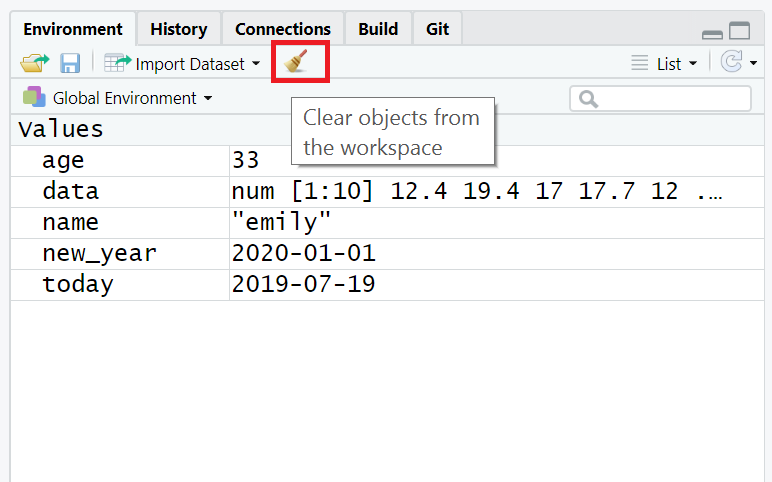
\includegraphics[width=1\linewidth]{images/broom} 

}

\caption{Clearing the workspace}\label{fig:img-broom}
\end{figure}

\hypertarget{r-uxe7alux131ux15fma-dizini}{%
\section{R Çalışma Dizini}\label{r-uxe7alux131ux15fma-dizini}}

\begin{itemize}
\item
  R yazılımı Start/Baslangic menusu üzerinden çalıştırıldığında çalışma dizini \textbf{C:/Users//Documents}
\item
  Çalışma dizinini sorgulamak için kullanılacak olan fonksiyon

  \begin{itemize}
  \tightlist
  \item
    \texttt{getwd()} (get working directory)
  \end{itemize}
\item
  Çalışma dizinini değiştirmek için kullanılacak olan fonksiyon

  \begin{itemize}
  \tightlist
  \item
    \texttt{setwd()} (set working directory)
  \end{itemize}
\item
  Bu işlem Rstudio menusu \textbf{``Session''} sekmesinden ya da \textbf{CTRL +Shift + H} tuşları ile de yapılabilmektedir.
\end{itemize}

\hypertarget{ri-kapatma}{%
\section{R'i Kapatma}\label{ri-kapatma}}

\begin{itemize}
\item
  Kaydet (Save) ya da CTLR + S \texttt{dosyadi.R} uzantısıyla kaydedilebilmektedir.
\item
  Bu sayede tekrar kullanılabilmekte ya da başkaları ile kolaylıkla paylaşılabilmektedir.
\item
  Tüm programlar gibi \textbf{``x''} işareti ile ya da \textbf{q()} fonksiyonunu ile sonlandırılabilir.
\item
  R'dan çıkış yaparken, program çalışma alanının kaydedilip kaydedilmeyeceğini sormaktadır.
\item
  Eger R'in çalışma alanını kaydetmesini istenirse, R çalışma dizinine `.Rdata uzantılı bir dosya kaydeder.
\item
  Çalışma alanı kaydı için \texttt{save.image("dosyaadi")} komutu da kullanılabilmektedir.
\item
  R'dan çıkış yapmadan yapılan işlem durdurulmak istenirse, konsol bölümündeki \textbf{``Stop''} işareti veya \textbf{Esc} tuşları kullanılabilir.
\end{itemize}

\hypertarget{r-kaynaklarux131}{%
\section{R Kaynakları}\label{r-kaynaklarux131}}

\begin{itemize}
\tightlist
\item
  🔗\href{https://cran.r*\%20project.org/web/views/Psychometrics.html}{Alana ozgu paketler}
\item
  Paket yardım sayfaları ve paket vignetteleri
\item
  e* posta gruplarindaki e* postalara \texttt{RSiteSearch\ ("sample.int")} ''
\item
  \texttt{ltm\ reliability} gibi fonskiyon isimler argumansiz kullanirlirsa icerigi gorunur. Karmasik gorunse de siz de yapabilirsiniz. Öğrenmek için iyi bir yoldur.
\item
  🔗\url{https://www.learnr4free.com/tr/index.html}
\item
  🔗\href{https://cran.r-project.org/doc/contrib/Short-refcard.pdf}{Referans kartları}
\item
  🔗\href{https://www.rstudio.com/resources/cheatsheets/}{Cheat Sheets}
\item
  🔗\href{https://hadley.nz/}{Hadley Wickham}
\item
  🔗\href{http://r4stats.com/}{rforstats}
\item
  🔗\href{https://blog.revolutionanalytics.com/r*\%20is*\%20hot/}{r is hot}
\item
  🔗\href{http://www.matthewckeller.com/}{paralel programlama}
\end{itemize}

\hypertarget{uxf6dev-1}{%
\section{Ödev}\label{uxf6dev-1}}

\begin{itemize}
\item
  Sadece temel pakette 1500'e yakın fonksiyon bulunduğu için ders dışı alıştırmalar yapmanız gereklidir.
\item
  \href{https://learnr-examples.shinyapps.io/ex-setup-r/}{R kurulumu ile ilgili} learnr paketi hazırlanmış bir interaktif alıştırma örneğini inceleyeniz.
\item
  Kitap Bölüm 1 alıştırmalarını tamamlayınız.
\item
  Datacamp da üzerine atanan bölüm alıştırmalarını tamamlayınız.
\item
  swirl package \textbf{learn R in R} paketi yükleyerek alıştırma yapmayı deneyiniz.
\item
  \href{https://cran.r-project.org/doc/contrib/Short-refcard.pdf}{Referens kart} sayfasının çıktısını alarak duvarınıza asmanızı öneririm.
\end{itemize}

\hypertarget{r-oturumlarux131}{%
\section{R oturumları}\label{r-oturumlarux131}}

\begin{itemize}
\tightlist
\item
  R'yi açıp kod yazmaya, paketleri yüklemeye ve nesneler oluşturmaya başladığınızda, bunu yeni bir \textbf{oturumda} yaparsınız. Çalışma alanını temizlemeye ek olarak, bazen yeni bir oturum başlatmak yararlı olabilir. Bu, bilgisayarınızda R'yi her başlattığınızda otomatik olarak gerçekleşir, ancak oturumlar sunucuda kalıcı olabilir. Kodunuzun çalışmadığını fark ederseniz ve nedenini bulamazsanız, yeni bir oturum başlatmaya değer olabilir. Bu, ortamı temizleyecek ve yüklü tüm paketleri ayıracaktır - bunu telefonunuzu yeniden başlatmak gibi düşünün.
\end{itemize}

\hypertarget{alux131ux15ftux131rma}{%
\section{Alıştırma}\label{alux131ux15ftux131rma}}

'Oturum - R'yi Yeniden Başlat'a tıklayın.

\begin{figure}

{\centering 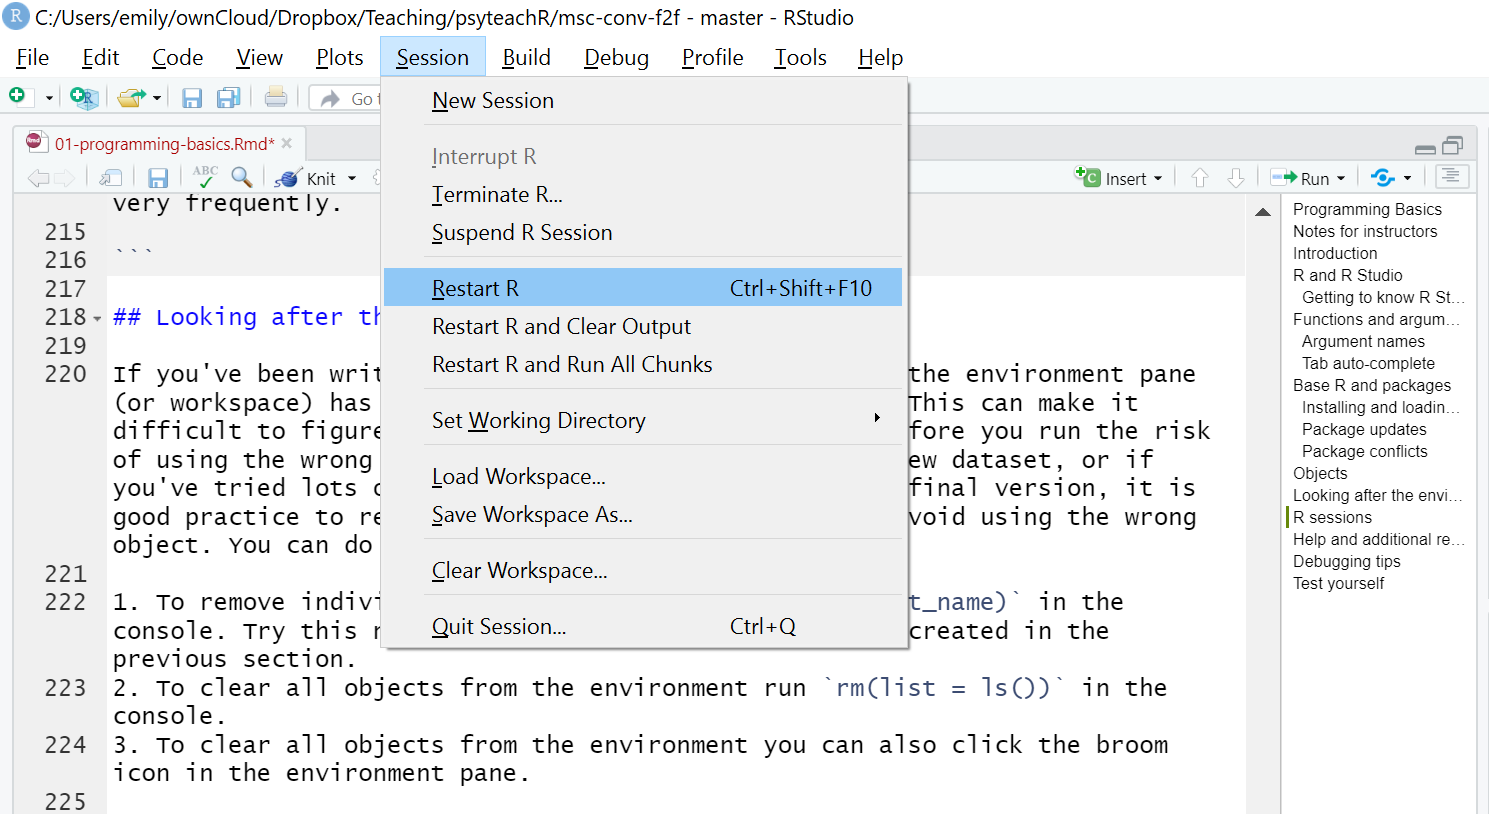
\includegraphics[width=1\linewidth]{images/new_session} 

}

\caption{The truth about programming}\label{fig:img-session}
\end{figure}

\hypertarget{hata-ayux131klama-ipuuxe7larux131}{%
\section{Hata ayıklama ipuçları}\label{hata-ayux131klama-ipuuxe7larux131}}

-Kodlamanın büyük bir kısmı kodunuzun neden çalışmadığını anlamaya çalışmaktır ve bu acemi ya da uzman olmanız fark etmeksizin geçerlidir.

\begin{itemize}
\item
  Bu kurs boyunca ilerlerken yaptığınız hataların ve bunları nasıl düzelttiğinizin kaydını tutmalısınız.
\item
  Her bölümde dikkat etmeniz gereken bir dizi yaygın hata sunacağız, ancak şüphesiz kendiniz de yeni hatalar yapacaksınız (ve düzelteceksiniz!).
\item
  Kullanmaya çalıştığınız fonksiyonlar için doğru paketleri yüklediniz mi? Çok yaygın bir hata, paketi yüklemek için kodu yazmaktır, örneğin \texttt{library(tidyverse)} ancak daha sonra çalıştırmayı unutmaktır.
\item
  Bir yazım hatası mı yaptınız? Unutmayın \texttt{data} ile \texttt{DATA} aynı şey değildir ve \texttt{t.test} ile \texttt{t\_test} aynı şey değildir.
\item
  Bir paket çakışması mı var? Paket ve fonksiyonu \texttt{package::function} ile belirtmeyi denediniz mi?
\item
  Bu kesinlikle bir hata mı? R'deki tüm kırmızı metinler hata anlamına gelmez - bazen size sadece bilgi içeren bir mesaj verir.
\end{itemize}

\hypertarget{yardux131mcux131-kaynaklar}{%
\section{Yardımcı Kaynaklar}\label{yardux131mcux131-kaynaklar}}

Programlamada iyi olmak demek, bir şeyler denemek, internette yardım aramak ve kopyalanacak kod örnekleri bulmak demektir. B

\begin{itemize}
\item
  etkili bir şekilde problem çözmeyi öğrenmek, bu kurs boyunca geliştirmeniz gereken temel bir beceridir.
\item
  Yardım belgelerini kullanın. Bir fonksiyonun nasıl çalıştığını anlamakta zorlanıyorsanız, \texttt{?function} komutunu hatırlayın.
\item
  Bir hata mesajı alırsanız, kopyalayıp Google'a yapıştırın - büyük olasılıkla başka biri de aynı sorunu yaşamıştır.
\item
  Bu ders materyallerine ek olarak, R öğrenmek için bir dizi mükemmel kaynak vardır:

  \begin{itemize}
  \tightlist
  \item
    \href{http://www.cookbook-r.com/}{R Cookbook}
  \item
    \href{https://stackoverflow.com/}{StackOverflow}
  \item
    \href{https://r4ds.had.co.nz/}{Veri Bilimi için R}
  \item
    Twitter'da \href{https://twitter.com/search?f=tweets\&q=\%23rstats\&src=typd}{\#rstats} hashtag'ini arayın veya kullanın
  \end{itemize}
\end{itemize}

\hypertarget{alux131ux15ftux131rma-kendini-test-et}{%
\section{Alıştırma : Kendini test et}\label{alux131ux15ftux131rma-kendini-test-et}}

\textbf{Soru 1.} Neden \texttt{install.packages()} kodunu analiz kodlarında asla dahil \textbf{etmemelisiniz}?

\begin{itemize}
\item
  \begin{enumerate}
  \def\labelenumi{(\Alph{enumi})}
  \tightlist
  \item
    Bunun yerine library() kullanmalısınız\\
  \end{enumerate}
\item
  \begin{enumerate}
  \def\labelenumi{(\Alph{enumi})}
  \setcounter{enumi}{1}
  \tightlist
  \item
    Paketler zaten temel R'ın bir parçasıdır\\
  \end{enumerate}
\item
  \begin{enumerate}
  \def\labelenumi{(\Alph{enumi})}
  \setcounter{enumi}{2}
  \tightlist
  \item
    Siz (veya bir başkası) yanlışlıkla kodunuzun çalışmasını durduran bir paket güncellemesi yükleyebilirsiniz\\
  \end{enumerate}
\item
  \begin{enumerate}
  \def\labelenumi{(\Alph{enumi})}
  \setcounter{enumi}{3}
  \tightlist
  \item
    Paketin en son sürümüne zaten sahipsiniz
  \end{enumerate}
\end{itemize}

Açıklama

Unutmayın, \texttt{install.packages()} işlevini çalıştırdığınızda her zaman paketin en son sürümü yüklenir ve yüklemiş olabileceğiniz eski sürümlerin üzerine yazılır.

\textbf{Soru 2.}Aşağıdaki kod ne üretecektir?

\begin{Shaded}
\begin{Highlighting}[]
\FunctionTok{rnorm}\NormalTok{(}\DecValTok{6}\NormalTok{, }\DecValTok{50}\NormalTok{, }\DecValTok{10}\NormalTok{)}
\end{Highlighting}
\end{Shaded}

\begin{itemize}
\item
  \begin{enumerate}
  \def\labelenumi{(\Alph{enumi})}
  \tightlist
  \item
    Ortalaması 6 ve SD'si 50 olan 10 sayıdan oluşan bir veri seti\\
  \end{enumerate}
\item
  \begin{enumerate}
  \def\labelenumi{(\Alph{enumi})}
  \setcounter{enumi}{1}
  \tightlist
  \item
    Ortalaması 50 ve SD'si 10 olan 6 sayıdan oluşan bir veri seti\\
  \end{enumerate}
\item
  \begin{enumerate}
  \def\labelenumi{(\Alph{enumi})}
  \setcounter{enumi}{2}
  \tightlist
  \item
    Ortalaması 10 ve SD'si 6 olan 50 sayıdan oluşan bir veri seti\\
  \end{enumerate}
\item
  \begin{enumerate}
  \def\labelenumi{(\Alph{enumi})}
  \setcounter{enumi}{3}
  \tightlist
  \item
    Ortalaması 10 ve SD'si 6 olan 50 sayıdan oluşan bir veri seti
  \end{enumerate}
\end{itemize}

Açıklama

\texttt{rnorm()} için varsayılan biçim \texttt{rnorm(n,\ mean,\ sd)} şeklindedir. Bir fonksiyonun her bir argümanının ne işe yaradığını hatırlamak için yardıma ihtiyacınız varsa, \texttt{?rnorm} komutunu çalıştırarak yardım belgelerine bakın

\textbf{Soru 3.} Aynı isimde fonksiyonlara sahip iki paketiniz varsa ve tam olarak hangi paketin kullanılacağını belirtmek istiyorsanız, hangi kodu kullanırsınız?

\begin{itemize}
\item
  \begin{enumerate}
  \def\labelenumi{(\Alph{enumi})}
  \tightlist
  \item
    package::function\\
  \end{enumerate}
\item
  \begin{enumerate}
  \def\labelenumi{(\Alph{enumi})}
  \setcounter{enumi}{1}
  \tightlist
  \item
    function::package\\
  \end{enumerate}
\item
  \begin{enumerate}
  \def\labelenumi{(\Alph{enumi})}
  \setcounter{enumi}{2}
  \tightlist
  \item
    library(package)\\
  \end{enumerate}
\item
  \begin{enumerate}
  \def\labelenumi{(\Alph{enumi})}
  \setcounter{enumi}{3}
  \tightlist
  \item
    install.packages(package)
  \end{enumerate}
\end{itemize}

Açıklama

Örneğin \texttt{dplyr::select} gibi \texttt{package::function} biçimini kullanmalısınız. Paketlerinizi ilk yüklediğinizde, herhangi bir fonksiyon aynı isme sahipse R'nin sizi uyaracağını unutmayın - buna dikkat etmeyi unutmayın!

\textbf{Soru 4.} Aşağıdakilerden hangisinin bir arguman olması en muhtemeldir?

\begin{itemize}
\item
  \begin{enumerate}
  \def\labelenumi{(\Alph{enumi})}
  \tightlist
  \item
    35\\
  \end{enumerate}
\item
  \begin{enumerate}
  \def\labelenumi{(\Alph{enumi})}
  \setcounter{enumi}{1}
  \tightlist
  \item
    read\_csv()\\
  \end{enumerate}
\item
  \begin{enumerate}
  \def\labelenumi{(\Alph{enumi})}
  \setcounter{enumi}{2}
  \tightlist
  \item
    \textless-
  \end{enumerate}
\end{itemize}

\textbf{Soru 5.} Fonksiyonları belirlemenin kolay bir yolu aşağıdakilerden hangisine bakmaktır

\begin{itemize}
\item
  \begin{enumerate}
  \def\labelenumi{(\Alph{enumi})}
  \tightlist
  \item
    ()\\
  \end{enumerate}
\item
  \begin{enumerate}
  \def\labelenumi{(\Alph{enumi})}
  \setcounter{enumi}{1}
  \tightlist
  \item
    {[}{]}\\
  \end{enumerate}
\item
  \begin{enumerate}
  \def\labelenumi{(\Alph{enumi})}
  \setcounter{enumi}{2}
  \tightlist
  \item
    \{\}
  \end{enumerate}
\end{itemize}

.

\textbf{Soru 6.} \textless-`'nin görevi, fonksiyondan elde edilen çıktıyı bir/bir \ldots\ldots\ldots\ldots\ldots\ldots\ldots{} atamaktır.

\begin{itemize}
\item
  \begin{enumerate}
  \def\labelenumi{(\Alph{enumi})}
  \tightlist
  \item
    nesne\\
  \end{enumerate}
\item
  \begin{enumerate}
  \def\labelenumi{(\Alph{enumi})}
  \setcounter{enumi}{1}
  \tightlist
  \item
    atama\\
  \end{enumerate}
\item
  \begin{enumerate}
  \def\labelenumi{(\Alph{enumi})}
  \setcounter{enumi}{2}
  \tightlist
  \item
    arguman
  \end{enumerate}
\end{itemize}

.

\hypertarget{r-nesneler}{%
\chapter{R Nesneler}\label{r-nesneler}}

\begin{itemize}
\tightlist
\item
  Örnek bir veri seti
\end{itemize}

\begin{Shaded}
\begin{Highlighting}[]
\FunctionTok{library}\NormalTok{(tidyverse)}
\FunctionTok{data}\NormalTok{(diamonds)}
\FunctionTok{head}\NormalTok{(diamonds)}
\end{Highlighting}
\end{Shaded}

\begin{verbatim}
## # A tibble: 6 x 10
##   carat cut       color clarity depth table price     x     y     z
##   <dbl> <ord>     <ord> <ord>   <dbl> <dbl> <int> <dbl> <dbl> <dbl>
## 1  0.23 Ideal     E     SI2      61.5    55   326  3.95  3.98  2.43
## 2  0.21 Premium   E     SI1      59.8    61   326  3.89  3.84  2.31
## 3  0.23 Good      E     VS1      56.9    65   327  4.05  4.07  2.31
## 4  0.29 Premium   I     VS2      62.4    58   334  4.2   4.23  2.63
## 5  0.31 Good      J     SI2      63.3    58   335  4.34  4.35  2.75
## 6  0.24 Very Good J     VVS2     62.8    57   336  3.94  3.96  2.48
\end{verbatim}

R nesne (object) yönelimli bir programlama dilidir.

\begin{itemize}
\tightlist
\item
  Karakter (character)
\item
  Sayısal (numeric)

  \begin{itemize}
  \tightlist
  \item
    tam sayı (integer)
  \item
    ondalıklı sayı (double)
  \item
    karmaşık sayı (complex)
  \end{itemize}
\item
  Mantıksal (logical)
\item
  Faktör (factor)
\item
  Liste (list)
\item
  Fonksiyon (function)
\end{itemize}

\hypertarget{tam-sayi}{%
\section{tam sayi}\label{tam-sayi}}

\begin{itemize}
\tightlist
\item
  tamsayı nesnesi oluşturulması
\end{itemize}

\begin{Shaded}
\begin{Highlighting}[]
\NormalTok{tamsayi }\OtherTok{\textless{}{-}}\NormalTok{ 2L}
\end{Highlighting}
\end{Shaded}

\begin{itemize}
\tightlist
\item
  tamsayi nesnesinin türünün sorgulanması
\end{itemize}

\begin{Shaded}
\begin{Highlighting}[]
\FunctionTok{typeof}\NormalTok{(tamsayi)}
\end{Highlighting}
\end{Shaded}

\begin{verbatim}
## [1] "integer"
\end{verbatim}

\begin{itemize}
\tightlist
\item
  tamsayı nesnesinin yazdırılması
\end{itemize}

\begin{Shaded}
\begin{Highlighting}[]
\NormalTok{tamsayi}
\end{Highlighting}
\end{Shaded}

\begin{verbatim}
## [1] 2
\end{verbatim}

\hypertarget{ondalux131k-sayux131}{%
\section{ondalık sayı}\label{ondalux131k-sayux131}}

\begin{itemize}
\tightlist
\item
  ondaliksayi nesnesinin oluşturulması
\end{itemize}

\begin{Shaded}
\begin{Highlighting}[]
\NormalTok{ondaliksayi }\OtherTok{\textless{}{-}} \FloatTok{2.5}
\end{Highlighting}
\end{Shaded}

\begin{itemize}
\tightlist
\item
  ondaliksayi nesnesinin türünün sorgulanması
\end{itemize}

\begin{Shaded}
\begin{Highlighting}[]
\FunctionTok{typeof}\NormalTok{(ondaliksayi)}
\end{Highlighting}
\end{Shaded}

\begin{verbatim}
## [1] "double"
\end{verbatim}

\begin{itemize}
\tightlist
\item
  ondaliksayi nesnesinin yazdırılması
\end{itemize}

\begin{Shaded}
\begin{Highlighting}[]
\NormalTok{ondaliksayi}
\end{Highlighting}
\end{Shaded}

\begin{verbatim}
## [1] 2.5
\end{verbatim}

\hypertarget{iux15flemler}{%
\section{İşlemler}\label{iux15flemler}}

\begin{itemize}
\tightlist
\item
  tek elemanlı vektörler
\end{itemize}

\begin{Shaded}
\begin{Highlighting}[]
\NormalTok{x }\OtherTok{\textless{}{-}} \DecValTok{1}
\NormalTok{y }\OtherTok{\textless{}{-}} \DecValTok{1}
\end{Highlighting}
\end{Shaded}

\begin{Shaded}
\begin{Highlighting}[]
\NormalTok{x}\SpecialCharTok{+}\NormalTok{y}
\end{Highlighting}
\end{Shaded}

\begin{verbatim}
## [1] 2
\end{verbatim}

\begin{itemize}
\tightlist
\item
  çok elemanlı vektörler
\end{itemize}

\begin{Shaded}
\begin{Highlighting}[]
\NormalTok{x }\OtherTok{\textless{}{-}} \FunctionTok{c}\NormalTok{(}\DecValTok{3}\NormalTok{,}\DecValTok{4}\NormalTok{,}\DecValTok{5}\NormalTok{)}
\NormalTok{y }\OtherTok{\textless{}{-}} \FunctionTok{c}\NormalTok{(}\DecValTok{1}\NormalTok{,}\DecValTok{2}\NormalTok{,}\DecValTok{3}\NormalTok{)}
\CommentTok{\# vektör eleman sayıları aynı mı?}
\FunctionTok{length}\NormalTok{(x)}\SpecialCharTok{==}\FunctionTok{length}\NormalTok{(y)}
\end{Highlighting}
\end{Shaded}

\begin{verbatim}
## [1] TRUE
\end{verbatim}

\begin{Shaded}
\begin{Highlighting}[]
\NormalTok{x}\SpecialCharTok{+}\NormalTok{y}
\end{Highlighting}
\end{Shaded}

\begin{verbatim}
## [1] 4 6 8
\end{verbatim}

\begin{Shaded}
\begin{Highlighting}[]
\NormalTok{x}\SpecialCharTok{{-}}\NormalTok{y}
\end{Highlighting}
\end{Shaded}

\begin{verbatim}
## [1] 2 2 2
\end{verbatim}

\begin{itemize}
\tightlist
\item
  çok elemanlı vektörler
\end{itemize}

\begin{Shaded}
\begin{Highlighting}[]
\NormalTok{x }\OtherTok{\textless{}{-}} \DecValTok{1}\SpecialCharTok{:}\DecValTok{9}
\NormalTok{y }\OtherTok{\textless{}{-}} \FunctionTok{c}\NormalTok{(}\DecValTok{1}\NormalTok{,}\DecValTok{2}\NormalTok{,}\DecValTok{3}\NormalTok{)}
\CommentTok{\# vektör eleman sayıları farklı mı?}
\FunctionTok{length}\NormalTok{(x)}\SpecialCharTok{/}\FunctionTok{length}\NormalTok{(y)}
\end{Highlighting}
\end{Shaded}

\begin{verbatim}
## [1] 3
\end{verbatim}

\begin{Shaded}
\begin{Highlighting}[]
\NormalTok{x}\SpecialCharTok{+}\NormalTok{y}
\end{Highlighting}
\end{Shaded}

\begin{verbatim}
## [1]  2  4  6  5  7  9  8 10 12
\end{verbatim}

\begin{Shaded}
\begin{Highlighting}[]
\NormalTok{x}\SpecialCharTok{/}\NormalTok{y}
\end{Highlighting}
\end{Shaded}

\begin{verbatim}
## [1] 1.0 1.0 1.0 4.0 2.5 2.0 7.0 4.0 3.0
\end{verbatim}

\begin{itemize}
\tightlist
\item
  çok elemanlı vektörler
\end{itemize}

\begin{Shaded}
\begin{Highlighting}[]
\NormalTok{x }\OtherTok{\textless{}{-}} \DecValTok{1}\SpecialCharTok{:}\DecValTok{5}
\NormalTok{y }\OtherTok{\textless{}{-}} \FunctionTok{c}\NormalTok{(}\DecValTok{1}\NormalTok{,}\DecValTok{2}\NormalTok{)}
\CommentTok{\# vektör eleman sayıları farklı olduğunda}
\FunctionTok{length}\NormalTok{(x)}\SpecialCharTok{/}\FunctionTok{length}\NormalTok{(y)}
\end{Highlighting}
\end{Shaded}

\begin{verbatim}
## [1] 2.5
\end{verbatim}

\begin{itemize}
\tightlist
\item
  \texttt{x+y} işleminin sonucu nedir? \_\_\_\_\_\_\_\_\_
\end{itemize}

Çözüm

\begin{Shaded}
\begin{Highlighting}[]
\NormalTok{x }\SpecialCharTok{+}\NormalTok{ y}
\end{Highlighting}
\end{Shaded}

\begin{verbatim}
## Warning in x + y: longer object length is not a multiple of shorter object
## length
\end{verbatim}

\begin{verbatim}
## [1] 2 4 4 6 6
\end{verbatim}

\hypertarget{karakter-nesneler}{%
\section{Karakter Nesneler}\label{karakter-nesneler}}

\begin{itemize}
\tightlist
\item
  karakter nesnesi oluşturulması
\end{itemize}

\begin{Shaded}
\begin{Highlighting}[]
\NormalTok{karakter }\OtherTok{\textless{}{-}} \StringTok{"olcme"}
\end{Highlighting}
\end{Shaded}

\begin{itemize}
\tightlist
\item
  Oluşturulan nesnenin türünün sorgulanmasa
\end{itemize}

\begin{Shaded}
\begin{Highlighting}[]
\FunctionTok{typeof}\NormalTok{(karakter)}
\end{Highlighting}
\end{Shaded}

\begin{verbatim}
## [1] "character"
\end{verbatim}

\begin{itemize}
\tightlist
\item
  nesne yazdırılması
\end{itemize}

\begin{Shaded}
\begin{Highlighting}[]
\NormalTok{karakter}
\end{Highlighting}
\end{Shaded}

\begin{verbatim}
## [1] "olcme"
\end{verbatim}

\begin{Shaded}
\begin{Highlighting}[]
\CommentTok{\# karakter nesnesi oluşturulması}
\NormalTok{ad }\OtherTok{\textless{}{-}} \StringTok{"Su"}
\NormalTok{soyad }\OtherTok{\textless{}{-}} \StringTok{"Sevim"}
\end{Highlighting}
\end{Shaded}

\begin{itemize}
\tightlist
\item
  iki nesneyi arada boşluk bırakarak birleştirir.
\end{itemize}

\begin{Shaded}
\begin{Highlighting}[]
\FunctionTok{paste}\NormalTok{(ad,soyad)}
\end{Highlighting}
\end{Shaded}

\begin{verbatim}
## [1] "Su Sevim"
\end{verbatim}

\begin{itemize}
\tightlist
\item
  sep argümanı farklı şekillerde özelleştirilebilir.
\end{itemize}

\begin{Shaded}
\begin{Highlighting}[]
\FunctionTok{paste}\NormalTok{(ad,soyad, }\AttributeTok{sep=}\StringTok{""}\NormalTok{)}
\end{Highlighting}
\end{Shaded}

\begin{verbatim}
## [1] "SuSevim"
\end{verbatim}

\begin{Shaded}
\begin{Highlighting}[]
\FunctionTok{paste}\NormalTok{(ad,soyad,}\AttributeTok{sep=}\StringTok{"\_"}\NormalTok{)}
\end{Highlighting}
\end{Shaded}

\begin{verbatim}
## [1] "Su_Sevim"
\end{verbatim}

\begin{itemize}
\tightlist
\item
  base pakette yer alan bazı karakter vektörler bulunmaktadır.
\end{itemize}

\begin{Shaded}
\begin{Highlighting}[]
\NormalTok{letters}
\end{Highlighting}
\end{Shaded}

\begin{verbatim}
##  [1] "a" "b" "c" "d" "e" "f" "g" "h" "i" "j" "k" "l" "m" "n" "o" "p" "q" "r" "s"
## [20] "t" "u" "v" "w" "x" "y" "z"
\end{verbatim}

\begin{Shaded}
\begin{Highlighting}[]
\NormalTok{LETTERS}
\end{Highlighting}
\end{Shaded}

\begin{verbatim}
##  [1] "A" "B" "C" "D" "E" "F" "G" "H" "I" "J" "K" "L" "M" "N" "O" "P" "Q" "R" "S"
## [20] "T" "U" "V" "W" "X" "Y" "Z"
\end{verbatim}

\begin{Shaded}
\begin{Highlighting}[]
\NormalTok{month.name}
\end{Highlighting}
\end{Shaded}

\begin{verbatim}
##  [1] "January"   "February"  "March"     "April"     "May"       "June"     
##  [7] "July"      "August"    "September" "October"   "November"  "December"
\end{verbatim}

\begin{Shaded}
\begin{Highlighting}[]
\NormalTok{month.abb}
\end{Highlighting}
\end{Shaded}

\begin{verbatim}
##  [1] "Jan" "Feb" "Mar" "Apr" "May" "Jun" "Jul" "Aug" "Sep" "Oct" "Nov" "Dec"
\end{verbatim}

\begin{itemize}
\tightlist
\item
  Nesne birleştirme fonksiyonlarından en sık kullananı \texttt{paste()}
\item
  \texttt{paste()} fonksiyonunun temel argümanları ise \texttt{sep} ve \texttt{collapse}'dir.
\end{itemize}

\begin{Shaded}
\begin{Highlighting}[]
\NormalTok{harf5}\OtherTok{\textless{}{-}}\NormalTok{ letters[}\DecValTok{1}\SpecialCharTok{:}\DecValTok{5}\NormalTok{]}
\NormalTok{(harf51 }\OtherTok{\textless{}{-}} \FunctionTok{paste}\NormalTok{(harf5,}\DecValTok{1}\SpecialCharTok{:}\DecValTok{5}\NormalTok{,}\AttributeTok{sep=}\StringTok{"\_"}\NormalTok{))}
\end{Highlighting}
\end{Shaded}

\begin{verbatim}
## [1] "a_1" "b_2" "c_3" "d_4" "e_5"
\end{verbatim}

\begin{Shaded}
\begin{Highlighting}[]
\FunctionTok{length}\NormalTok{(harf51)}
\end{Highlighting}
\end{Shaded}

\begin{verbatim}
## [1] 5
\end{verbatim}

\begin{Shaded}
\begin{Highlighting}[]
\NormalTok{(harf52 }\OtherTok{\textless{}{-}} \FunctionTok{paste}\NormalTok{(harf5,}\DecValTok{1}\SpecialCharTok{:}\DecValTok{5}\NormalTok{,}\AttributeTok{sep=}\StringTok{"\_"}\NormalTok{,}
                 \AttributeTok{collapse=}\StringTok{" "}\NormalTok{))}
\end{Highlighting}
\end{Shaded}

\begin{verbatim}
## [1] "a_1 b_2 c_3 d_4 e_5"
\end{verbatim}

\begin{Shaded}
\begin{Highlighting}[]
\FunctionTok{length}\NormalTok{(harf52)}
\end{Highlighting}
\end{Shaded}

\begin{verbatim}
## [1] 1
\end{verbatim}

\begin{itemize}
\tightlist
\item
  \texttt{paste()} fonksiyonun yardım sayfasını inceleyiniz.
\end{itemize}

\hypertarget{guxfcnuxfcn-sorusu}{%
\subsection{Günün Sorusu}\label{guxfcnuxfcn-sorusu}}

\begin{itemize}
\tightlist
\item
  Aşağıdaki çıktıyı oluşturacak olan kodu oluşturunuz.
\end{itemize}

\begin{verbatim}
##  [1] "1. maddenin guclugu: 0.52"  "2. maddenin guclugu: 0.88" 
##  [3] "3. maddenin guclugu: 0.21"  "4. maddenin guclugu: 0.67" 
##  [5] "5. maddenin guclugu: 0.69"  "6. maddenin guclugu: 0.8"  
##  [7] "7. maddenin guclugu: 0.11"  "8. maddenin guclugu: 0.35" 
##  [9] "9. maddenin guclugu: 0.16"  "10. maddenin guclugu: 0.75"
\end{verbatim}

Bunun birden fazla yolu olabilir, farklı şekillerde yapabilirsiniz.

\textbf{Büyük Küçük Harf Düzenleme Fonksiyonları} \texttt{toupper()} ve \texttt{tolower()}

\begin{Shaded}
\begin{Highlighting}[]
\FunctionTok{toupper}\NormalTok{(harf5)}
\end{Highlighting}
\end{Shaded}

\begin{verbatim}
## [1] "A" "B" "C" "D" "E"
\end{verbatim}

\begin{Shaded}
\begin{Highlighting}[]
\FunctionTok{tolower}\NormalTok{(harf5)}
\end{Highlighting}
\end{Shaded}

\begin{verbatim}
## [1] "a" "b" "c" "d" "e"
\end{verbatim}

\texttt{casefold()} fonksiyonu da upper argümanı ile birlikte kullanılabilir.

\begin{Shaded}
\begin{Highlighting}[]
\FunctionTok{casefold}\NormalTok{(harf5, }\AttributeTok{upper =} \ConstantTok{FALSE}\NormalTok{)}
\end{Highlighting}
\end{Shaded}

\begin{verbatim}
## [1] "a" "b" "c" "d" "e"
\end{verbatim}

\begin{Shaded}
\begin{Highlighting}[]
\FunctionTok{casefold}\NormalTok{(harf5, }\AttributeTok{upper =} \ConstantTok{TRUE}\NormalTok{)}
\end{Highlighting}
\end{Shaded}

\begin{verbatim}
## [1] "A" "B" "C" "D" "E"
\end{verbatim}

\begin{itemize}
\tightlist
\item
  Karakter nesnelerin kaç harften oluştuğu \texttt{nchar()} fonksiyonu ile belirlenebilir.
\end{itemize}

\begin{Shaded}
\begin{Highlighting}[]
\FunctionTok{nchar}\NormalTok{(month.name)}
\end{Highlighting}
\end{Shaded}

\begin{verbatim}
##  [1] 7 8 5 5 3 4 4 6 9 7 8 8
\end{verbatim}

\begin{itemize}
\tightlist
\item
  Karakter nesneleri belli bir yerden bölmek icin \texttt{substr()} ve \texttt{substring()} fonksiyonları kullanılabilir.
\end{itemize}

\begin{Shaded}
\begin{Highlighting}[]
\FunctionTok{substr}\NormalTok{(}\StringTok{"YILMAZ"}\NormalTok{, }\DecValTok{1}\NormalTok{,}\DecValTok{3}\NormalTok{)}
\end{Highlighting}
\end{Shaded}

\begin{verbatim}
## [1] "YIL"
\end{verbatim}

\begin{itemize}
\item
  \texttt{substring("YILMAZ",\ 1:..\ ,\ 1:6)} kodunda ``Y'' ``I'' ``L'' ``M'' ``A'' ``Z'' çıktısı oluşturacak kodu yazınız \_
\item
  `\texttt{substring("YILMAZ",\ ...\ ,\ 4:6)} kodunda ``ILM'' ``ILMA'' ``ILMAZ''` çıktınısı oluşturacak kodu yazınız \_
\item
  Karakter nesnelerde daha fazlası için aşağıdaki fonksiyonları inceleyebilirsiniz.
\item
  \texttt{strsplit()}
\item
  \texttt{noquote()}
\item
  \texttt{cat()}
\item
  \texttt{grep()}
\item
  \texttt{duplicated()}
\item
  \texttt{agrep()}
\end{itemize}

\hypertarget{mantux131ksal-nesneler}{%
\section{Mantıksal Nesneler}\label{mantux131ksal-nesneler}}

\begin{Shaded}
\begin{Highlighting}[]
\NormalTok{mantiksal1 }\OtherTok{\textless{}{-}}\ConstantTok{TRUE}
\end{Highlighting}
\end{Shaded}

\begin{Shaded}
\begin{Highlighting}[]
\FunctionTok{typeof}\NormalTok{(mantiksal1)}
\end{Highlighting}
\end{Shaded}

\begin{verbatim}
## [1] "logical"
\end{verbatim}

\begin{Shaded}
\begin{Highlighting}[]
\NormalTok{mantiksal1}
\end{Highlighting}
\end{Shaded}

\begin{verbatim}
## [1] TRUE
\end{verbatim}

Mantıksal operatörler programlamanın temeli ve vazgeçilmezidir.

\begin{Shaded}
\begin{Highlighting}[]
\CommentTok{\# eşitlik sınaması}
\NormalTok{T}\SpecialCharTok{==}\ConstantTok{TRUE}
\end{Highlighting}
\end{Shaded}

\begin{verbatim}
## [1] TRUE
\end{verbatim}

\begin{itemize}
\item
  \texttt{4==5} kodunun sonucu nedir? \_\_\_\_\_
\item
  \texttt{4\textless{}5} kodunun sonucu nedir? \_\_\_\_
\item
  \texttt{10\textgreater{}100} kodunun sonucu nedir? \_\_\_\_\_
\item
  Mantıksal operatörlerle yapılan sınamalar ile mantıksal nesneler oluşturulur.
\end{itemize}

\begin{Shaded}
\begin{Highlighting}[]
\NormalTok{sonuc }\OtherTok{\textless{}{-}} \DecValTok{4}\SpecialCharTok{\textless{}}\DecValTok{5}
\FunctionTok{typeof}\NormalTok{(sonuc)}
\end{Highlighting}
\end{Shaded}

\begin{verbatim}
## [1] "logical"
\end{verbatim}

\begin{itemize}
\tightlist
\item
  Nesne türleri arasındaki değişim uygunluk durumuna göre \texttt{as.*()}fonksiyonları ile sağlanır.
\end{itemize}

\begin{Shaded}
\begin{Highlighting}[]
\CommentTok{\# Karakter veri numerik veriye}
\FunctionTok{as.numeric}\NormalTok{(}\StringTok{"3.14"}\NormalTok{)}
\end{Highlighting}
\end{Shaded}

\begin{verbatim}
## [1] 3.14
\end{verbatim}

\begin{Shaded}
\begin{Highlighting}[]
\CommentTok{\# ondalık verin tam sayıya}
\FunctionTok{as.integer}\NormalTok{(pi)}
\end{Highlighting}
\end{Shaded}

\begin{verbatim}
## [1] 3
\end{verbatim}

\begin{Shaded}
\begin{Highlighting}[]
\CommentTok{\# karakter veri numerik veriye (NA)}
\FunctionTok{as.numeric}\NormalTok{(}\StringTok{"olcme"}\NormalTok{)}
\end{Highlighting}
\end{Shaded}

\begin{verbatim}
## Warning: NAs introduced by coercion
\end{verbatim}

\begin{verbatim}
## [1] NA
\end{verbatim}

\begin{Shaded}
\begin{Highlighting}[]
\CommentTok{\# mantıksal veri karakter veriye (NA)}
\FunctionTok{as.character}\NormalTok{(}\ConstantTok{TRUE}\NormalTok{)}
\end{Highlighting}
\end{Shaded}

\begin{verbatim}
## [1] "TRUE"
\end{verbatim}

\begin{Shaded}
\begin{Highlighting}[]
\CommentTok{\# numerik veri karakter veriye}
\FunctionTok{as.character}\NormalTok{(}\DecValTok{10}\NormalTok{)}
\end{Highlighting}
\end{Shaded}

\begin{verbatim}
## [1] "10"
\end{verbatim}

\begin{Shaded}
\begin{Highlighting}[]
\CommentTok{\# mantıksal veri numerik veriye}
\FunctionTok{as.numeric}\NormalTok{(}\ConstantTok{TRUE}\NormalTok{)}
\end{Highlighting}
\end{Shaded}

\begin{verbatim}
## [1] 1
\end{verbatim}

\hypertarget{nesne-tuxfcrleri-sorgulama}{%
\section{Nesne Türleri Sorgulama}\label{nesne-tuxfcrleri-sorgulama}}

\begin{itemize}
\tightlist
\item
  Nesne türleri sorgulamak için ise \texttt{class()} ya da \texttt{mode()} fonksiyonları kullanabilir. Ancak bir nesne türüne ait olup olmadığını sorgulamak için ise \texttt{is.*()} fonksiyonları kullanılır.
\end{itemize}

\begin{Shaded}
\begin{Highlighting}[]
\NormalTok{x}\OtherTok{\textless{}{-}} \FloatTok{3.14}\NormalTok{; }\FunctionTok{class}\NormalTok{(x)}
\end{Highlighting}
\end{Shaded}

\begin{verbatim}
## [1] "numeric"
\end{verbatim}

\begin{Shaded}
\begin{Highlighting}[]
\FunctionTok{is.numeric}\NormalTok{(x)}
\end{Highlighting}
\end{Shaded}

\begin{verbatim}
## [1] TRUE
\end{verbatim}

\begin{Shaded}
\begin{Highlighting}[]
\FunctionTok{is.logical}\NormalTok{(x)}
\end{Highlighting}
\end{Shaded}

\begin{verbatim}
## [1] FALSE
\end{verbatim}

\begin{itemize}
\tightlist
\item
  Sayısal nesnelerin türü için \texttt{typeof()} fonksiyonu da kullanılabilir.
\end{itemize}

\begin{Shaded}
\begin{Highlighting}[]
\NormalTok{y }\OtherTok{\textless{}{-}}\NormalTok{ 2L; }\FunctionTok{typeof}\NormalTok{(y); }\FunctionTok{class}\NormalTok{(y) }\CommentTok{\# satir içi kod ayırma}
\end{Highlighting}
\end{Shaded}

\begin{verbatim}
## [1] "integer"
## [1] "integer"
\end{verbatim}

\begin{Shaded}
\begin{Highlighting}[]
\FunctionTok{is.integer}\NormalTok{(y)}
\end{Highlighting}
\end{Shaded}

\begin{verbatim}
## [1] TRUE
\end{verbatim}

\begin{Shaded}
\begin{Highlighting}[]
\FunctionTok{is.double}\NormalTok{(y)}
\end{Highlighting}
\end{Shaded}

\begin{verbatim}
## [1] FALSE
\end{verbatim}

\hypertarget{guxfcnuxfcn-sorusu-1}{%
\subsection{Günün Sorusu}\label{guxfcnuxfcn-sorusu-1}}

\begin{itemize}
\tightlist
\item
  aşağıda yer alan \textbf{ad\_soyad} nesnesini kullanarak
\end{itemize}

\begin{Shaded}
\begin{Highlighting}[]
\NormalTok{ad\_soyad}\OtherTok{\textless{}{-}} \FunctionTok{c}\NormalTok{(}\StringTok{"Ayse{-}Sel"}\NormalTok{,}\StringTok{"Can{-}Yucel"}\NormalTok{,}\StringTok{"Cem{-}Togay"}\NormalTok{,}\StringTok{"Banu{-}Cift"}\NormalTok{)}
\end{Highlighting}
\end{Shaded}

aşağıdaki çıktıyı oluşturmaya calisiniz.

\begin{verbatim}
## [1] "Ayse" "Can"  "Cem"  "Banu"
## [1] "Sel"   "Yucel" "Togay" "Cift"
\end{verbatim}

\hypertarget{vektuxf6rler}{%
\chapter{Vektörler}\label{vektuxf6rler}}

\begin{itemize}
\item
  R lineer cebir temelli bir programlama dilidir.
\item
  Vektörler tek boyutludur.
\item
  R'da vektörler birleştirmek (combine/concatenate) anlamına gelen \texttt{c()} fonksiyonu ile oluşturulmaktadır.
\item
  R da veriler bir araya gelerek veri yapılarını oluşturur.

  \begin{itemize}
  \tightlist
  \item
    vektör (vector)
  \item
    liste (list)
  \item
    matris (matrix)
  \item
    veri seti (data.frame)
  \item
    dizi (array)
  \end{itemize}
\end{itemize}

\hypertarget{vektuxf6r-oluux15fturma}{%
\section{Vektör Oluşturma}\label{vektuxf6r-oluux15fturma}}

\begin{Shaded}
\begin{Highlighting}[]
\NormalTok{(sayisal\_vektor }\OtherTok{\textless{}{-}}  \FunctionTok{c}\NormalTok{(}\DecValTok{1}\NormalTok{,}\DecValTok{2}\NormalTok{,}\DecValTok{3}\NormalTok{))}
\end{Highlighting}
\end{Shaded}

\begin{verbatim}
## [1] 1 2 3
\end{verbatim}

\begin{Shaded}
\begin{Highlighting}[]
\NormalTok{(karakter\_vektor }\OtherTok{\textless{}{-}}  \FunctionTok{c}\NormalTok{(}\StringTok{"a"}\NormalTok{,}\StringTok{"b"}\NormalTok{,}\StringTok{"c"}\NormalTok{))  }\DocumentationTok{\#\# cift tirnak}
\end{Highlighting}
\end{Shaded}

\begin{verbatim}
## [1] "a" "b" "c"
\end{verbatim}

\begin{Shaded}
\begin{Highlighting}[]
\NormalTok{(mantiksal\_vektor }\OtherTok{\textless{}{-}} \FunctionTok{c}\NormalTok{(}\ConstantTok{TRUE}\NormalTok{,}\ConstantTok{TRUE}\NormalTok{,}\ConstantTok{FALSE}\NormalTok{))}
\end{Highlighting}
\end{Shaded}

\begin{verbatim}
## [1]  TRUE  TRUE FALSE
\end{verbatim}

\hypertarget{vektuxf6r-iux15flemleri}{%
\section{Vektör İşlemleri}\label{vektuxf6r-iux15flemleri}}

\begin{itemize}
\item
  Vektör uzunluğu \texttt{length()} fonksiyonu ile vektör türleri ise \texttt{class()}, \texttt{mode()} ya da \texttt{typeof()} fonksiyonları ise tur belirlemek için kullanılmaktadır.
\item
  Vektörler bir veya daha fazla elemandan oluşabilmektedir.
\end{itemize}

\begin{Shaded}
\begin{Highlighting}[]
\NormalTok{a }\OtherTok{\textless{}{-}} \DecValTok{1}  \CommentTok{\# tek elemandan oluşur.}
\CommentTok{\# Vektör uzunluğunu öğrenmek icin length() fonksiyonu}
\FunctionTok{length}\NormalTok{(a)}
\end{Highlighting}
\end{Shaded}

\begin{verbatim}
## [1] 1
\end{verbatim}

\begin{Shaded}
\begin{Highlighting}[]
\NormalTok{x }\OtherTok{\textless{}{-}} \DecValTok{1}\SpecialCharTok{:}\DecValTok{10}
\end{Highlighting}
\end{Shaded}

\begin{itemize}
\item
  bir vektöründeki verilerin toplanması \texttt{sum(x)} 55
\item
  bir vektöründeki verilerin çarpılması \texttt{prod(x)} \ensuremath{3.6288\times 10^{6}}
\item
  bir vektöründeki verilerin küçükten büyüğe sıralanması \texttt{sort(x)} 1, 2, 3, 4, 5, 6, 7, 8, 9, 10
\item
  bir vektörünün elemanların sıralarının tersine çevrilmesi \texttt{rev(x)} 10, 9, 8, 7, 6, 5, 4, 3, 2, 1
\item
  bir vektöründeki verilerin standart sapmasının hesaplanması \texttt{sd(x)} 3.0276504
\item
  bir vektöründeki en büyük verinin gösterilmesi \texttt{max(x)} 10
\item
  bir vektöründeki en küçük verinin gösterilmesi \texttt{min(x)} 1
\item
  En büyük verinin vektörün kaçıncı elemanı olduğunun gösterilmesi \texttt{which.max(x)} 10
\item
  En küçük verinin vektörün kaçıncı elemanı olduğunun gösterilmesi \texttt{which.min(x)} 1
\item
  Vektörlerden eleman sırası, isim ve mantıksal operatörler olmak üzere üç farklı yolla eleman seçilebilir.
\end{itemize}

\begin{Shaded}
\begin{Highlighting}[]
\NormalTok{ad  }\OtherTok{\textless{}{-}}  \FunctionTok{c}\NormalTok{(}\StringTok{"Ali"}\NormalTok{,}\StringTok{"Elif"}\NormalTok{,}\StringTok{"Su"}\NormalTok{,}\StringTok{"Deniz"}\NormalTok{,}
\StringTok{"Aras"}\NormalTok{,}\StringTok{"Berk"}\NormalTok{,}\StringTok{"Can"}\NormalTok{,}\StringTok{"Ece"}\NormalTok{,}\StringTok{"Efe"}\NormalTok{,}\StringTok{"Arda"}\NormalTok{)}
\end{Highlighting}
\end{Shaded}

\begin{itemize}
\item
  ad vektörünün 1. elemanı \texttt{ad{[}1{]}} Ali
\item
  ad vektörünün 5. elemanını yazdıracak kodu oluşturunuz. \_\_\_\_\_
\item
  ad vektörünün son elemanını yazdıracak kodu oluşturunuz. \_\_\_\_\_\_
\item
  ad vektörünün son elemanını yazdıracak kodu vektörün 10 elemanlı olduğunu bilmediğiniz de ne yaparsınız? \_\_\_\_\_\_\_\_\_\_\_\_\_\_
\item
  Vektörün sadece 1., 5. 8 elemanının yazdıracak kodu oluşturunuz.\_\_\_\_\_\_\_\_\_\_\_\_
\item
  Vektörün sadece 1. elemanının hariç tutacak kodu oluşturunuz \_\_\_\_\_\_
\item
  Vektörün 1. ve 5. elemanının hariç tutacak kodu oluşturunuz \_\_\_\_\_\_\_\_\_\_\_
\item
  Vektörün son üç elemanını yazdıracak kodu oluşturunuz \texttt{r}fitb(``ad{[}8:10{]}'')`
\end{itemize}

\hypertarget{vektuxf6re-eleman-eklenmesi}{%
\section{Vektöre eleman eklenmesi}\label{vektuxf6re-eleman-eklenmesi}}

\begin{Shaded}
\begin{Highlighting}[]
\NormalTok{ad[}\DecValTok{11}\NormalTok{] }\OtherTok{\textless{}{-}} \StringTok{"Asu"}\NormalTok{; ad}
\end{Highlighting}
\end{Shaded}

\begin{verbatim}
##  [1] "Ali"   "Elif"  "Su"    "Deniz" "Aras"  "Berk"  "Can"   "Ece"   "Efe"  
## [10] "Arda"  "Asu"
\end{verbatim}

\begin{itemize}
\tightlist
\item
  vektöre birden fazla eleman eklenmesi
\end{itemize}

\begin{Shaded}
\begin{Highlighting}[]
\NormalTok{ad[}\DecValTok{12}\SpecialCharTok{:}\DecValTok{13}\NormalTok{] }\OtherTok{\textless{}{-}} \FunctionTok{c}\NormalTok{(}\StringTok{"Ahu"}\NormalTok{,}\StringTok{"Han"}\NormalTok{); ad}
\end{Highlighting}
\end{Shaded}

\begin{verbatim}
##  [1] "Ali"   "Elif"  "Su"    "Deniz" "Aras"  "Berk"  "Can"   "Ece"   "Efe"  
## [10] "Arda"  "Asu"   "Ahu"   "Han"
\end{verbatim}

\begin{itemize}
\tightlist
\item
  Vektörün ortasına eleman eklenmesi \textbf{append()} fonksiyonu ile yapılabilir. Fonksiyon yardım sayfasını inceleyiniz.
\end{itemize}

\begin{Shaded}
\begin{Highlighting}[]
\NormalTok{(ad }\OtherTok{\textless{}{-}} \FunctionTok{append}\NormalTok{(ad, }\StringTok{"Taha"}\NormalTok{, }\AttributeTok{after =} \DecValTok{3}\NormalTok{))}
\end{Highlighting}
\end{Shaded}

\begin{verbatim}
##  [1] "Ali"   "Elif"  "Su"    "Taha"  "Deniz" "Aras"  "Berk"  "Can"   "Ece"  
## [10] "Efe"   "Arda"  "Asu"   "Ahu"   "Han"
\end{verbatim}

\begin{itemize}
\tightlist
\item
  ya da \texttt{c()} fonksiyonu ile yapılabilir.
\end{itemize}

\begin{Shaded}
\begin{Highlighting}[]
\NormalTok{ad }\OtherTok{\textless{}{-}} \FunctionTok{c}\NormalTok{(ad[}\DecValTok{1}\SpecialCharTok{:}\DecValTok{5}\NormalTok{],}\StringTok{"Selim"}\NormalTok{,ad[}\DecValTok{7}\SpecialCharTok{:}\FunctionTok{length}\NormalTok{(ad)]); ad}
\end{Highlighting}
\end{Shaded}

\begin{verbatim}
##  [1] "Ali"   "Elif"  "Su"    "Taha"  "Deniz" "Selim" "Berk"  "Can"   "Ece"  
## [10] "Efe"   "Arda"  "Asu"   "Ahu"   "Han"
\end{verbatim}

\hypertarget{alux131ux15ftux131rma-1}{%
\section{Alıştırma}\label{alux131ux15ftux131rma-1}}

\begin{itemize}
\tightlist
\item
  10 kişiden oluşan bir gruptaki kişilerinin boy ve kilo ölçümleri için ise aşağıdaki vektör oluşturulmuştur.
\end{itemize}

\begin{Shaded}
\begin{Highlighting}[]
\NormalTok{ad  }\OtherTok{\textless{}{-}}  \FunctionTok{c}\NormalTok{(}\StringTok{"Ali"}\NormalTok{,}\StringTok{"Elif"}\NormalTok{,}\StringTok{"Su"}\NormalTok{,}\StringTok{"Deniz"}\NormalTok{,}
\StringTok{"Aras"}\NormalTok{,}\StringTok{"Berk"}\NormalTok{,}\StringTok{"Can"}\NormalTok{,}\StringTok{"Ece"}\NormalTok{,}\StringTok{"Efe"}\NormalTok{,}\StringTok{"Arda"}\NormalTok{)}
\NormalTok{boy }\OtherTok{\textless{}{-}} \FunctionTok{c}\NormalTok{(}\DecValTok{160}\NormalTok{,}\DecValTok{165}\NormalTok{,}\DecValTok{170}\NormalTok{,}\DecValTok{155}\NormalTok{,}\DecValTok{167}\NormalTok{,}\DecValTok{162}\NormalTok{,}\DecValTok{169}\NormalTok{,}\DecValTok{158}\NormalTok{,}\DecValTok{160}\NormalTok{,}\DecValTok{164}\NormalTok{)}
\NormalTok{kilo }\OtherTok{\textless{}{-}}\FunctionTok{c}\NormalTok{(}\DecValTok{50}\NormalTok{,}\DecValTok{55}\NormalTok{,}\DecValTok{57}\NormalTok{,}\DecValTok{50}\NormalTok{,}\DecValTok{48}\NormalTok{,}\DecValTok{65}\NormalTok{,}\DecValTok{58}\NormalTok{,}\DecValTok{62}\NormalTok{,}\DecValTok{45}\NormalTok{,}\DecValTok{47}\NormalTok{)}
\end{Highlighting}
\end{Shaded}

\begin{itemize}
\tightlist
\item
  Eğer elimizdeki vektör isimlendirilmiş bir vektör ise eleman seçimini isimle de yapabiliriz.
\end{itemize}

\begin{Shaded}
\begin{Highlighting}[]
\CommentTok{\#isimsiz boy vektoru}
\FunctionTok{names}\NormalTok{(boy) }\CommentTok{\# names() fonksiyonu ile isimlendirme yapılabilir.}
\end{Highlighting}
\end{Shaded}

\begin{verbatim}
## NULL
\end{verbatim}

\begin{itemize}
\item
  ad vektörünü boy vektörünü isimlendirirken nasıl kullanabiliriz? \_\_\_\_\_\_\_\_\_\_\_\_\_\_\_\_
\item
  Arda 'nın boyunu isimlendirilmiş vektörü kullanarak nasıl yazdırırsınız? \texttt{r}fitb(``boy{[}''Arda''{]}'')`
\end{itemize}

\hypertarget{uxf6ruxfcntuxfclerle-vektuxf6r-oluux15fturma}{%
\section{Örüntülerle Vektör Oluşturma}\label{uxf6ruxfcntuxfclerle-vektuxf6r-oluux15fturma}}

\begin{itemize}
\item
  Vektör oluşturmanın farklı yolları bulunmaktadır.
\item
  En basit yolu iki nokta \texttt{":"} operatörünü kullanmaktır.
\end{itemize}

\begin{Shaded}
\begin{Highlighting}[]
\NormalTok{rakamlar }\OtherTok{\textless{}{-}} \DecValTok{0}\SpecialCharTok{:}\DecValTok{9}
\NormalTok{rakamlar}
\end{Highlighting}
\end{Shaded}

\begin{verbatim}
##  [1] 0 1 2 3 4 5 6 7 8 9
\end{verbatim}

\begin{itemize}
\tightlist
\item
  büyükten küçüğe rakamlardan vektör oluşturulması
\end{itemize}

\begin{Shaded}
\begin{Highlighting}[]
\NormalTok{rakamlar }\OtherTok{\textless{}{-}} \DecValTok{9}\SpecialCharTok{:}\DecValTok{0}
\NormalTok{rakamlar}
\end{Highlighting}
\end{Shaded}

\begin{verbatim}
##  [1] 9 8 7 6 5 4 3 2 1 0
\end{verbatim}

\hypertarget{seq}{%
\subsection{seq()}\label{seq}}

\begin{itemize}
\item
  Belirli bir kurala göre sayı dizileri oluşturmak için ise \texttt{seq()}, \texttt{rep()} ve \texttt{paste()} fonksiyonlarından yararlanılabilir. İlk olarak bu fonksiyonların yardım sayfalarını inceleyelim.
\item
  1'den 10'a kadar birer birer artan sayılardan dizi oluşturulacak kodu oluşturunuz. \texttt{seq(from=1,to=10,by=...)} \_
\item
  Bir önceki işlemi argümansız olarak oluşturunuz. \_\_\_\_\_\_\_\_\_\_\_
\item
  Aynı çıktıyı tek bir argümanla elde edebilir misiniz? \_\_\_\_\_\_\_\_\_\_
\item
  length argümanını kullanarak aşağıdaki çıktıyı oluşturacak kodu oluşturunuz. \_\_\_\_\_\_\_\_\_\_\_\_\_\_\_\_\_\_\_\_\_\_\_\_\_
\end{itemize}

\begin{verbatim}
## [1] 1.0 1.4 1.8 2.2 2.6 3.0
\end{verbatim}

\begin{itemize}
\tightlist
\item
  by argümanını ile artış miktarını kullanarak aşağıdaki çıktıyı oluşturacak kodu oluşturunuz. \_\_\_\_\_\_\_\_\_\_\_\_\_\_\_\_\_\_\_\_\_\_\_
\end{itemize}

\begin{verbatim}
## [1] 1.0 1.5 2.0 2.5 3.0
\end{verbatim}

\begin{itemize}
\tightlist
\item
  Belirli bir aralıkta kaç elemanın yer alacağını length.out argümanı kullanarak aşağıdaki çıktıyı oluşturacak kodu oluşturunuz. \_\_\_\_\_\_\_\_\_\_\_\_\_\_\_\_\_\_\_\_\_\_\_\_\_\_\_\_\_
\end{itemize}

\begin{verbatim}
## [1] 1.0 1.5 2.0 2.5 3.0
\end{verbatim}

\hypertarget{rep}{%
\subsection{rep()}\label{rep}}

\texttt{rep()} fonksiyonu için örnekler

\begin{Shaded}
\begin{Highlighting}[]
\CommentTok{\# üç elemanlı bir vektörün üç kere tekrar ettirilmesi}
\FunctionTok{rep}\NormalTok{(}\FunctionTok{c}\NormalTok{(}\DecValTok{3}\NormalTok{,}\DecValTok{4}\NormalTok{,}\DecValTok{5}\NormalTok{), }\DecValTok{3}\NormalTok{)}
\end{Highlighting}
\end{Shaded}

\begin{verbatim}
## [1] 3 4 5 3 4 5 3 4 5
\end{verbatim}

\begin{Shaded}
\begin{Highlighting}[]
\CommentTok{\# rakamların üç kere tekrar ettirilmesi}
\FunctionTok{rep}\NormalTok{(}\DecValTok{0}\SpecialCharTok{:}\DecValTok{9}\NormalTok{, }\AttributeTok{times =} \DecValTok{3}\NormalTok{) }
\end{Highlighting}
\end{Shaded}

\begin{verbatim}
##  [1] 0 1 2 3 4 5 6 7 8 9 0 1 2 3 4 5 6 7 8 9 0 1 2 3 4 5 6 7 8 9
\end{verbatim}

\begin{itemize}
\tightlist
\item
  \texttt{a\ \textless{}-\ c(3,5,7)} vektörünü kullanarak aşağıdaki çıktıyı elde edecek kodu hazırlayınız. \_\_\_\_\_\_\_\_\_\_\_\_\_
\end{itemize}

\begin{verbatim}
## [1] 3 3 3 5 5 5 7 7 7
\end{verbatim}

\begin{itemize}
\tightlist
\item
  \texttt{a\ \textless{}-\ c(3,5,7)} vektörünü kullanarak aşağıdaki çıktıyı elde edecek kodu hazırlayınız. \_\_\_\_\_\_\_\_\_\_\_\_\_\_\_\_\_\_\_\_\_
\end{itemize}

\begin{verbatim}
##  [1] 3 3 3 5 5 5 7 7 7 3 3 3 5 5 5 7 7 7 3 3 3 5 5 5 7 7 7
\end{verbatim}

\begin{itemize}
\tightlist
\item
  Çıktıyı elde edecek kodu hazırlayınız. \_\_\_\_\_\_\_\_\_\_\_\_\_\_\_\_\_\_\_
\end{itemize}

\begin{verbatim}
## [1] 1 1 2 2 3 3 4 4
\end{verbatim}

\begin{itemize}
\tightlist
\item
  Çıktıyı elde edecek kodu hazırlayınız. \_\_\_\_\_\_\_\_\_\_\_\_
\end{itemize}

\begin{verbatim}
## [1] 1 2 2 3 3 3
\end{verbatim}

\hypertarget{paste}{%
\subsection{paste()}\label{paste}}

\begin{itemize}
\tightlist
\item
  \texttt{paste()}fonksiyonu çıktısı her zaman için karakterdir.
\end{itemize}

\begin{Shaded}
\begin{Highlighting}[]
\FunctionTok{paste}\NormalTok{(}\DecValTok{1}\SpecialCharTok{:}\DecValTok{4}\NormalTok{) }\CommentTok{\# çıktısı karakterdir}
\end{Highlighting}
\end{Shaded}

\begin{verbatim}
## [1] "1" "2" "3" "4"
\end{verbatim}

\begin{Shaded}
\begin{Highlighting}[]
\FunctionTok{class}\NormalTok{(}\FunctionTok{paste}\NormalTok{(}\DecValTok{1}\SpecialCharTok{:}\DecValTok{4}\NormalTok{))}
\end{Highlighting}
\end{Shaded}

\begin{verbatim}
## [1] "character"
\end{verbatim}

\begin{itemize}
\tightlist
\item
  Çıktıyı elde edecek kodu tamamlayınız \texttt{paste("test",...)} \_\_\_\_
\end{itemize}

\begin{verbatim}
##  [1] "test 1"  "test 2"  "test 3"  "test 4"  "test 5"  "test 6"  "test 7" 
##  [8] "test 8"  "test 9"  "test 10"
\end{verbatim}

\begin{itemize}
\tightlist
\item
  Çıktıyı elde edecek kodu tamamlayınız\texttt{paste("test",1:10,"...",sep="\_")} \_\_\_\_
\end{itemize}

\begin{verbatim}
##  [1] "test_1_puan"  "test_2_puan"  "test_3_puan"  "test_4_puan"  "test_5_puan" 
##  [6] "test_6_puan"  "test_7_puan"  "test_8_puan"  "test_9_puan"  "test_10_puan"
\end{verbatim}

\begin{itemize}
\tightlist
\item
  Çıktıyı elde edecek kodu tamamlayınız \texttt{paste("test",c("A","B","C","D",...))} \_\_\_
\end{itemize}

\begin{verbatim}
## [1] "test A" "test B" "test C" "test D" "test 1" "test 2" "test 3" "test 4"
\end{verbatim}

\hypertarget{rasgele-veri-oluux15fturma}{%
\section{Rasgele Veri Oluşturma}\label{rasgele-veri-oluux15fturma}}

\begin{itemize}
\tightlist
\item
  Farklı fonksiyonlarla rastgele veri üretilebilir. Örneğin 0-100 arasında 20 farklı değer elde edilmek istenilsin. Bunu yapmak için \texttt{sample()},\texttt{runif()} ya da \texttt{rnorm()} fonksiyonlarından yararlanılabilir.
\end{itemize}

\begin{Shaded}
\begin{Highlighting}[]
\FunctionTok{sample}\NormalTok{(}\DecValTok{0}\SpecialCharTok{:}\DecValTok{100}\NormalTok{,}\DecValTok{5}\NormalTok{)}
\end{Highlighting}
\end{Shaded}

\begin{verbatim}
## [1] 29 23 51 42 72
\end{verbatim}

\begin{Shaded}
\begin{Highlighting}[]
\FunctionTok{runif}\NormalTok{(}\DecValTok{10}\NormalTok{,  }\DecValTok{0}\NormalTok{, }\DecValTok{5}\NormalTok{)}
\end{Highlighting}
\end{Shaded}

\begin{verbatim}
##  [1] 1.40673901 0.57241018 2.17336066 3.96671890 2.68911204 4.51717755
##  [7] 1.64190804 0.65066983 4.30389799 0.09875575
\end{verbatim}

\begin{Shaded}
\begin{Highlighting}[]
\FunctionTok{rnorm}\NormalTok{(}\DecValTok{10}\NormalTok{,}\DecValTok{50}\NormalTok{,}\DecValTok{5}\NormalTok{)}
\end{Highlighting}
\end{Shaded}

\begin{verbatim}
##  [1] 49.08342 52.13135 50.98775 44.32830 49.60631 49.16930 42.16739 51.17894
##  [9] 59.22586 54.84551
\end{verbatim}

\begin{itemize}
\tightlist
\item
  Kullanılan üç fonksiyonun da yardım sayfalarını ve kullanım amaçlarını inceleyiniz.
\end{itemize}

\hypertarget{iux15flemler-1}{%
\section{İşlemler}\label{iux15flemler-1}}

BKI vücut ağırlığınızın metre cinsinden boy uzunluğunun karesine bölünmesi ile elde edilmektedir. Her bir bireye ait BKI değerini hesaplayınız. BKI derğerlerinin ortalaması kaçtır(iki ondalığa yuvarlayınız)? \_\_\_\_\_

\begin{Shaded}
\begin{Highlighting}[]
\NormalTok{ad  }\OtherTok{\textless{}{-}}  \FunctionTok{c}\NormalTok{(}\StringTok{"Ali"}\NormalTok{,}\StringTok{"Elif"}\NormalTok{,}\StringTok{"Su"}\NormalTok{,}\StringTok{"Deniz"}\NormalTok{,}\StringTok{"Aras"}\NormalTok{,}\StringTok{"Berk"}\NormalTok{,}\StringTok{"Can"}\NormalTok{,}\StringTok{"Ece"}\NormalTok{,}\StringTok{"Efe"}\NormalTok{,}\StringTok{"Arda"}\NormalTok{)}
\NormalTok{boy }\OtherTok{\textless{}{-}} \FunctionTok{c}\NormalTok{(}\DecValTok{160}\NormalTok{,}\DecValTok{165}\NormalTok{,}\DecValTok{170}\NormalTok{,}\DecValTok{155}\NormalTok{,}\DecValTok{167}\NormalTok{,}\DecValTok{162}\NormalTok{,}\DecValTok{169}\NormalTok{,}\DecValTok{158}\NormalTok{,}\DecValTok{160}\NormalTok{,}\DecValTok{164}\NormalTok{)}
\NormalTok{kilo }\OtherTok{\textless{}{-}} \FunctionTok{c}\NormalTok{(}\DecValTok{55}\NormalTok{,}\DecValTok{55}\NormalTok{,}\DecValTok{57}\NormalTok{,}\DecValTok{50}\NormalTok{,}\DecValTok{48}\NormalTok{,}\DecValTok{65}\NormalTok{,}\DecValTok{58}\NormalTok{,}\DecValTok{62}\NormalTok{,}\DecValTok{45}\NormalTok{,}\DecValTok{47}\NormalTok{)}
\end{Highlighting}
\end{Shaded}

Çözüm!,bakmadan yapmalısın!

\begin{Shaded}
\begin{Highlighting}[]
\CommentTok{\# BKI  hesaplanması}
\NormalTok{boy\_m  }\OtherTok{\textless{}{-}}\NormalTok{ boy}\SpecialCharTok{/}\DecValTok{100}
\NormalTok{BKI }\OtherTok{\textless{}{-}}\NormalTok{ kilo}\SpecialCharTok{/}\NormalTok{( boy\_m }\SpecialCharTok{*}\NormalTok{ boy\_m)}
\NormalTok{BKI}
\FunctionTok{round}\NormalTok{(}\FunctionTok{mean}\NormalTok{(BKI),}\DecValTok{2}\NormalTok{)}
\end{Highlighting}
\end{Shaded}

\begin{verbatim}
##  [1] 21.48437 20.20202 19.72318 20.81165 17.21109 24.76757 20.30741 24.83576
##  [9] 17.57812 17.47472
## [1] 20.44
\end{verbatim}

\hypertarget{kendinizi-test-edin}{%
\subsection{Kendinizi Test Edin}\label{kendinizi-test-edin}}

\textbf{S1.} Aşağıdaki tabloda yer alan üç sütun için birer vektör oluşturunuz. Öğrencilerin geçme notu her iki sınavın ortalaması olarak hesaplanacaktır. Bu öğrencilerin geçme notlarını hesaplayınız. Geçme notlarının betimsel istatistiklerini hesaplayınız.

\begin{longtable}[]{@{}lll@{}}
\toprule\noalign{}
Öğrenci & Vize & Final \\
\midrule\noalign{}
\endhead
\bottomrule\noalign{}
\endlastfoot
Ogrenci1 & 50 & 45 \\
Ogrenci2 & 55 & 65 \\
Ogrenci3 & 60 & 85 \\
Ogrenci4 & 70 & 90 \\
Ogrenci5 & 80 & 85 \\
\end{longtable}

Geçme notlarının minumum değeri: \_\_\_\_

Geçme notlarının ortalama değeri: \_\_\_\_

Geçme notlarının maksimum değeri: \_\_\_\_

\textbf{S2.} Birden n'e kadar olan sayların toplamını hesaplayan fonksiyon yazımı \texttt{toplam()} tek argümanlı fonksiyon oluşturunuz. Argüman değeri 5 olduğunda 1+2+3+4+5=15 değerini versin.

\begin{itemize}
\tightlist
\item
  birden n'e kadar olan sayların toplamı: (n*(n+1))/2
\end{itemize}

\textbf{S3.} 1'den n' e kadar olan sayıların toplamını hesaplayan fonksiyonu argümansız olarak aşağıdaki şekilde yazmayı deneyiniz. Fonksiyonu çalıştırdığınızda ekranda/konsolda kaça kadar olan sayların toplamı hesaplansın: yazsın, kullanıcının girdiği değere göre aşağıda çıktısı çıksın.

\begin{Shaded}
\begin{Highlighting}[]
\FunctionTok{toplam}\NormalTok{()}

\NormalTok{kaça kadar olan sayların toplamı hesaplansın}\SpecialCharTok{:} \DecValTok{10}

\NormalTok{[}\DecValTok{1} \StringTok{" 10 \textquotesingle{}e kadar olan sayların toplamı: 55}
\end{Highlighting}
\end{Shaded}

\hypertarget{odev}{%
\section{\texorpdfstring{\textbf{ODEV}}{ODEV}}\label{odev}}

\begin{itemize}
\item
  Kitap Bölüm 2 1. Soruyu tamamlayınız.
\item
  swirl package - learn R in R (Programming ilk 6 modul)
\item
  datacamp ödevinizi yapmayını unutmayın 😄
\end{itemize}

\hypertarget{veri-setleri}{%
\chapter{Veri Setleri}\label{veri-setleri}}

\begin{itemize}
\item
  Veri setleri iki boyutludur.
\item
  R'da bir çok fonksiyonun veri setleri ile çalışmaktadır.
\item
  Veri setleri R ortamında \texttt{data.frame()} fonksiyonu ile oluşturulabilir.
\item
  \texttt{data.frame()} fonksiyonu ile aynı uzunluktaki vektörlerden bir veri seti oluşturulabilir.
\end{itemize}

\begin{Shaded}
\begin{Highlighting}[]
\NormalTok{ad  }\OtherTok{\textless{}{-}}  \FunctionTok{c}\NormalTok{(}\StringTok{"Ali"}\NormalTok{,}\StringTok{"Elif"}\NormalTok{,}\StringTok{"Su"}\NormalTok{,}\StringTok{"Deniz"}\NormalTok{,}\StringTok{"Aras"}\NormalTok{, }\StringTok{"Berk"}\NormalTok{,}\StringTok{"Can"}\NormalTok{,}\StringTok{"Ece"}\NormalTok{,}\StringTok{"Efe"}\NormalTok{,}\StringTok{"Arda"}\NormalTok{)}
\NormalTok{boy }\OtherTok{\textless{}{-}} \FunctionTok{c}\NormalTok{(}\DecValTok{160}\NormalTok{,}\DecValTok{165}\NormalTok{,}\DecValTok{170}\NormalTok{,}\DecValTok{155}\NormalTok{,}\DecValTok{167}\NormalTok{,}\DecValTok{162}\NormalTok{, }\DecValTok{169}\NormalTok{,}\DecValTok{158}\NormalTok{,}\DecValTok{160}\NormalTok{,}\DecValTok{164}\NormalTok{)}
\NormalTok{kilo }\OtherTok{\textless{}{-}} \FunctionTok{c}\NormalTok{(}\DecValTok{55}\NormalTok{,}\DecValTok{55}\NormalTok{,}\DecValTok{57}\NormalTok{,}\DecValTok{50}\NormalTok{,}\DecValTok{48}\NormalTok{,}\DecValTok{65}\NormalTok{, }\DecValTok{58}\NormalTok{,}\DecValTok{62}\NormalTok{,}\DecValTok{45}\NormalTok{,}\DecValTok{47}\NormalTok{)}
\NormalTok{beden }\OtherTok{\textless{}{-}} \FunctionTok{c}\NormalTok{(}\StringTok{"S"}\NormalTok{,}\StringTok{"M"}\NormalTok{,}\StringTok{"S"}\NormalTok{,}\StringTok{"M"}\NormalTok{,}\StringTok{"S"}\NormalTok{, }\StringTok{"L"}\NormalTok{,}\StringTok{"M"}\NormalTok{,}\StringTok{"L"}\NormalTok{,}\StringTok{"S"}\NormalTok{,}\StringTok{"S"}\NormalTok{)}
\NormalTok{beden }\OtherTok{\textless{}{-}} \FunctionTok{factor}\NormalTok{(beden)}


\NormalTok{(df }\OtherTok{\textless{}{-}} \FunctionTok{data.frame}\NormalTok{(ad,boy, kilo, beden))}
\end{Highlighting}
\end{Shaded}

\begin{verbatim}
##       ad boy kilo beden
## 1    Ali 160   55     S
## 2   Elif 165   55     M
## 3     Su 170   57     S
## 4  Deniz 155   50     M
## 5   Aras 167   48     S
## 6   Berk 162   65     L
## 7    Can 169   58     M
## 8    Ece 158   62     L
## 9    Efe 160   45     S
## 10  Arda 164   47     S
\end{verbatim}

\begin{itemize}
\tightlist
\item
  Eğer uzunlukları farklı olan vektörlerle veri setleri oluşturulmaya çalışılırsa kısa vektör, uzun vektör uzunluğunda tekrar eder.
\end{itemize}

\begin{Shaded}
\begin{Highlighting}[]
\CommentTok{\# 4 farklı uzunlukta vektör oluşturulması}
\NormalTok{x }\OtherTok{\textless{}{-}} \DecValTok{11}\SpecialCharTok{:}\DecValTok{14}\NormalTok{; y }\OtherTok{\textless{}{-}} \DecValTok{10}\NormalTok{; M }\OtherTok{\textless{}{-}} \FunctionTok{c}\NormalTok{(}\DecValTok{10}\NormalTok{,}\DecValTok{35}\NormalTok{); N }\OtherTok{\textless{}{-}} \DecValTok{2}\SpecialCharTok{:}\DecValTok{4}
\end{Highlighting}
\end{Shaded}

\begin{Shaded}
\begin{Highlighting}[]
\FunctionTok{data.frame}\NormalTok{(x, y) }\CommentTok{\# (4,1)}
\end{Highlighting}
\end{Shaded}

\begin{verbatim}
##    x  y
## 1 11 10
## 2 12 10
## 3 13 10
## 4 14 10
\end{verbatim}

\begin{Shaded}
\begin{Highlighting}[]
\FunctionTok{data.frame}\NormalTok{(x, M) }\CommentTok{\# (4,2)}
\end{Highlighting}
\end{Shaded}

\begin{verbatim}
##    x  M
## 1 11 10
## 2 12 35
## 3 13 10
## 4 14 35
\end{verbatim}

\begin{Shaded}
\begin{Highlighting}[]
\FunctionTok{data.frame}\NormalTok{(x,N)  }\CommentTok{\#(4,3) hata}
\end{Highlighting}
\end{Shaded}

\begin{verbatim}
## Error in data.frame(x, N): arguments imply differing number of rows: 4, 3
\end{verbatim}

\begin{Shaded}
\begin{Highlighting}[]
\FunctionTok{data.frame}\NormalTok{(y, M) }\CommentTok{\#(1,2)}
\end{Highlighting}
\end{Shaded}

\begin{verbatim}
##    y  M
## 1 10 10
## 2 10 35
\end{verbatim}

\begin{Shaded}
\begin{Highlighting}[]
\FunctionTok{data.frame}\NormalTok{(y, N) }\CommentTok{\#(1,3)}
\end{Highlighting}
\end{Shaded}

\begin{verbatim}
##    y N
## 1 10 2
## 2 10 3
## 3 10 4
\end{verbatim}

\begin{Shaded}
\begin{Highlighting}[]
\FunctionTok{data.frame}\NormalTok{(M, N) }\CommentTok{\#(2,3)}
\end{Highlighting}
\end{Shaded}

\begin{verbatim}
## Error in data.frame(M, N): arguments imply differing number of rows: 2, 3
\end{verbatim}

\hypertarget{hazux131r-veri-setleri}{%
\section{Hazır Veri Setleri}\label{hazux131r-veri-setleri}}

\begin{itemize}
\tightlist
\item
  Temel pakette yer alan veri setlerinin bir listesine aşağıdaki komutla ulaşabilirsiniz.
\end{itemize}

\begin{Shaded}
\begin{Highlighting}[]
\FunctionTok{data}\NormalTok{() }\CommentTok{\# yeni bir pencerede açılır.}
\end{Highlighting}
\end{Shaded}

\begin{itemize}
\tightlist
\item
  Veri setlerinin yer aldığı paketlerde bulunmaktadır.
\end{itemize}

\begin{Shaded}
\begin{Highlighting}[]
\CommentTok{\# install.packages("datasets")}
\FunctionTok{library}\NormalTok{ (datasets)}
\CommentTok{\# install.packages("dslabs")}
\FunctionTok{library}\NormalTok{ (dslabs)}
\end{Highlighting}
\end{Shaded}

\begin{itemize}
\tightlist
\item
  Hazır veri setleri çalışma ortamına \texttt{data()} fonksiyonu ile aktarılabilir.
\end{itemize}

\begin{Shaded}
\begin{Highlighting}[]
\FunctionTok{data}\NormalTok{(WorldPhones) }\CommentTok{\# environmete kontrol ediniz. }
\end{Highlighting}
\end{Shaded}

\begin{itemize}
\tightlist
\item
  hazır veri setlerini incelememek için aşağıdaki komutlar kullanılabilir.
\end{itemize}

\begin{Shaded}
\begin{Highlighting}[]
\FunctionTok{data}\NormalTok{(cars) }\CommentTok{\# enviromente ekler}
\NormalTok{iris      }\CommentTok{\# enviromente eklemez!}
\end{Highlighting}
\end{Shaded}

\hypertarget{inceleme}{%
\section{İnceleme}\label{inceleme}}

\begin{itemize}
\tightlist
\item
  Boyut sorgulamamak için farklı fonksiyonlar kullanılabilir.
\end{itemize}

\begin{Shaded}
\begin{Highlighting}[]
\FunctionTok{dim}\NormalTok{(cars) }\CommentTok{\# satir Sutun}
\end{Highlighting}
\end{Shaded}

\begin{verbatim}
## [1] 50  2
\end{verbatim}

\begin{Shaded}
\begin{Highlighting}[]
\FunctionTok{nrow}\NormalTok{(cars)}
\end{Highlighting}
\end{Shaded}

\begin{verbatim}
## [1] 50
\end{verbatim}

\begin{Shaded}
\begin{Highlighting}[]
\FunctionTok{ncol}\NormalTok{(cars)}
\end{Highlighting}
\end{Shaded}

\begin{verbatim}
## [1] 2
\end{verbatim}

\begin{itemize}
\tightlist
\item
  Veri setlerin ilk satırları \texttt{head()}, son satırları ise \texttt{tail()} fonksiyonu ile incelenebilir. \texttt{head()} fonksiyonu olağan olarak ilk 6 satırı yazdırır.
\end{itemize}

\begin{Shaded}
\begin{Highlighting}[]
\FunctionTok{head}\NormalTok{(WorldPhones)}
\end{Highlighting}
\end{Shaded}

\begin{verbatim}
##      N.Amer Europe Asia S.Amer Oceania Africa Mid.Amer
## 1951  45939  21574 2876   1815    1646     89      555
## 1956  60423  29990 4708   2568    2366   1411      733
## 1957  64721  32510 5230   2695    2526   1546      773
## 1958  68484  35218 6662   2845    2691   1663      836
## 1959  71799  37598 6856   3000    2868   1769      911
## 1960  76036  40341 8220   3145    3054   1905     1008
\end{verbatim}

\begin{itemize}
\tightlist
\item
  Yazdırılacak satır sayısı \texttt{n} argümanı ile ayarlanır.
\end{itemize}

\begin{Shaded}
\begin{Highlighting}[]
\FunctionTok{head}\NormalTok{(WorldPhones,}\AttributeTok{n=}\DecValTok{2}\NormalTok{)}
\end{Highlighting}
\end{Shaded}

\begin{verbatim}
##      N.Amer Europe Asia S.Amer Oceania Africa Mid.Amer
## 1951  45939  21574 2876   1815    1646     89      555
## 1956  60423  29990 4708   2568    2366   1411      733
\end{verbatim}

\begin{itemize}
\item
  WorldPhones veri setinin son 8 satırını yazdıracak kodu yazınız. \_\_\_\_\_\_\_\_\_\_\_\_\_\_\_\_\_\_\_\_\_
\item
  \texttt{datasets} paketinde yer alan veri setlerinde \texttt{examples()} bölümünde çeşitli örneklere yer verilmiştir. Örneğin \texttt{example(WorldPhones)}
\end{itemize}

\begin{Shaded}
\begin{Highlighting}[]
\FunctionTok{matplot}\NormalTok{(}\FunctionTok{rownames}\NormalTok{(WorldPhones), WorldPhones, }\AttributeTok{type =} \StringTok{"b"}\NormalTok{, }\AttributeTok{log =} \StringTok{"y"}\NormalTok{,}
        \AttributeTok{xlab =} \StringTok{"Year"}\NormalTok{, }\AttributeTok{ylab =} \StringTok{"Number of telephones (1000\textquotesingle{}s)"}\NormalTok{)}
\FunctionTok{legend}\NormalTok{(}\StringTok{"bottomright"}\NormalTok{, }\FunctionTok{colnames}\NormalTok{(WorldPhones), }\AttributeTok{col =} \DecValTok{1}\SpecialCharTok{:}\DecValTok{6}\NormalTok{, }\AttributeTok{lty =} \DecValTok{1}\SpecialCharTok{:}\DecValTok{5}\NormalTok{,}
       \AttributeTok{pch =} \FunctionTok{rep}\NormalTok{(}\DecValTok{21}\NormalTok{, }\DecValTok{7}\NormalTok{))}
\FunctionTok{title}\NormalTok{(}\AttributeTok{main =} \StringTok{"World phones data: log scale for response"}\NormalTok{)}
\end{Highlighting}
\end{Shaded}

\begin{center}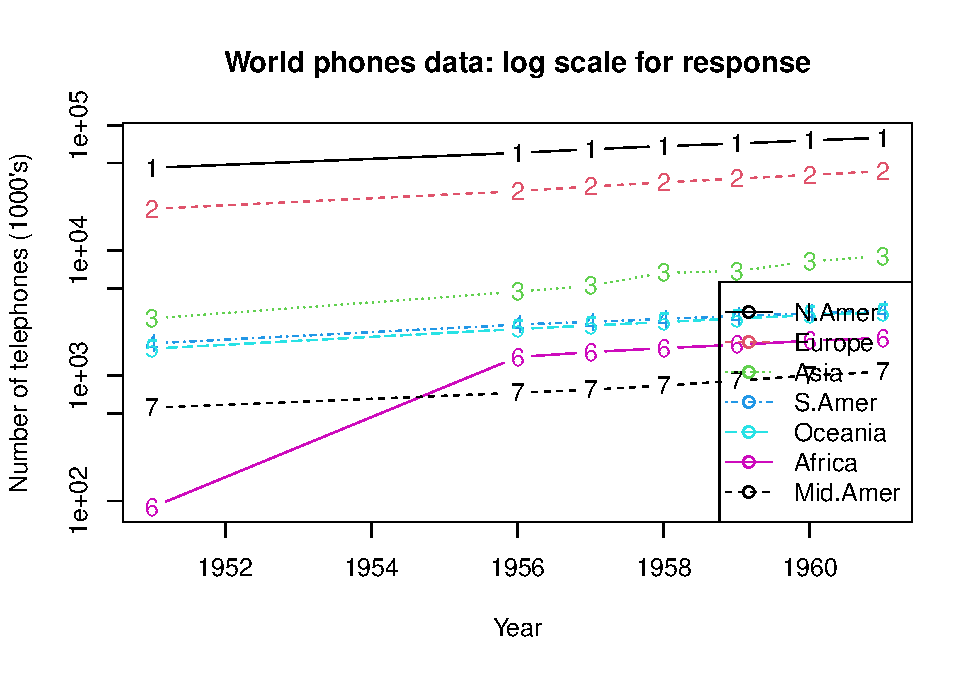
\includegraphics[width=1\linewidth]{06-veriseti_files/figure-latex/unnamed-chunk-18-1} \end{center}

\begin{itemize}
\tightlist
\item
  Temel paket hariç diğer paketlerdeki veri setlerine \texttt{data(veriseti,\ package="packagename")} şeklinde ulaşılabilir.
\end{itemize}

\begin{Shaded}
\begin{Highlighting}[]
\FunctionTok{data}\NormalTok{(CTTdata, }\AttributeTok{package=}\StringTok{"CTT"}\NormalTok{) }
\FunctionTok{head}\NormalTok{(CTTdata)}
\end{Highlighting}
\end{Shaded}

\begin{itemize}
\item
  🔗\href{http://r-tutorials.com/famous-useful-pre-installed-exercise-datasets-r/}{sık kullanılan veri setleri ile ilgili bir yazı:}
\item
  🔗\href{https://vincentarelbundock.github.io/Rdatasets/datasets.html}{tüm veri setlerine ulaşabilmek için ise:}
\item
  Kullanışlı olmasa da excel, spps gibi veri girişi sağlayan bir arayüz bulunmaktadır.
\item
  Ali, Su ve Ece'nin boylarının ve kilolarının seçilmesi
\end{itemize}

\begin{Shaded}
\begin{Highlighting}[]
\NormalTok{df1}\OtherTok{\textless{}{-}} \FunctionTok{data.frame}\NormalTok{() }
\NormalTok{df1 }\OtherTok{\textless{}{-}} \FunctionTok{edit}\NormalTok{(df1)}
\CommentTok{\# duzenlemek icin}
\FunctionTok{fix}\NormalTok{(df)}
\CommentTok{\# gozatmak icin }
\FunctionTok{View}\NormalTok{(df)}
\end{Highlighting}
\end{Shaded}

\hypertarget{elaman-seuxe7me}{%
\section{Elaman Seçme}\label{elaman-seuxe7me}}

Veri setlerinde eleman seçme matrislerdeki gibidir.

\texttt{df{[}satirindeks,\ sutunindeks{]}}

\begin{itemize}
\tightlist
\item
  df'nin birinci satir elemanlarının seçilmesi \_\_\_\_\_\_
\end{itemize}

\begin{verbatim}
##    ad boy kilo beden
## 1 Ali 160   55     S
\end{verbatim}

\begin{itemize}
\tightlist
\item
  df'nin birinci sütun elemanlarının seçilmesi \_\_\_\_\_\_
\end{itemize}

\begin{verbatim}
##  [1] "Ali"   "Elif"  "Su"    "Deniz" "Aras"  "Berk"  "Can"   "Ece"   "Efe"  
## [10] "Arda"
\end{verbatim}

\begin{itemize}
\tightlist
\item
  df'nin ikinci satir elemanlarının seçilmesi \_\_\_\_\_\_
\end{itemize}

\begin{verbatim}
##     ad boy kilo beden
## 2 Elif 165   55     M
\end{verbatim}

\begin{itemize}
\tightlist
\item
  df'nin ikinci sütun elemanlarının seçilmesi \_\_\_\_\_\_
\end{itemize}

\begin{verbatim}
##  [1] 160 165 170 155 167 162 169 158 160 164
\end{verbatim}

\begin{itemize}
\tightlist
\item
  df'nin birinci satir üçüncü sütun elemanlarının seçilmesi \_\_\_\_\_\_\_
\end{itemize}

\begin{verbatim}
## [1] 55
\end{verbatim}

\begin{itemize}
\tightlist
\item
  Veri setlerinde satır elemanları yazdırıldığında veri seti (\texttt{data.frame)}, sütun elemanları yazdırıldığında ise vektör (\texttt{vector)} oluşmaktadır.
\end{itemize}

\begin{Shaded}
\begin{Highlighting}[]
\CommentTok{\# satir secimi}
\FunctionTok{is.data.frame}\NormalTok{(df[}\DecValTok{1}\NormalTok{,])}
\end{Highlighting}
\end{Shaded}

\begin{verbatim}
## [1] TRUE
\end{verbatim}

\begin{Shaded}
\begin{Highlighting}[]
\CommentTok{\# sutun secimi}
\FunctionTok{is.data.frame}\NormalTok{(df[,}\DecValTok{1}\NormalTok{])}
\end{Highlighting}
\end{Shaded}

\begin{verbatim}
## [1] FALSE
\end{verbatim}

\begin{itemize}
\tightlist
\item
  Sütun seçimi veri seti (\texttt{data.frame}) olarak yapılmak istenirse, \texttt{drop} argümanı FALSE değeri ile kullanılır.
\end{itemize}

\begin{Shaded}
\begin{Highlighting}[]
\NormalTok{df[,}\DecValTok{1}\NormalTok{,drop}\OtherTok{=}\ConstantTok{FALSE}\NormalTok{]}
\end{Highlighting}
\end{Shaded}

\begin{verbatim}
##       ad
## 1    Ali
## 2   Elif
## 3     Su
## 4  Deniz
## 5   Aras
## 6   Berk
## 7    Can
## 8    Ece
## 9    Efe
## 10  Arda
\end{verbatim}

\begin{itemize}
\item
  Veri seçim işlemi için \texttt{subset()} fonksiyonu kullanılabilir.
\item
  \texttt{?subset} bir fonksiyonu ilk daha kullanıyorsanız, mutlaka yardım sayfasını inceleyin.
\end{itemize}

\texttt{subset(veriseti,\ kosul/Kosullar)}

\begin{itemize}
\tightlist
\item
  Boyu 165cm den uzun öğrencilerin bilgilerinin seçilmesi
\end{itemize}

\begin{Shaded}
\begin{Highlighting}[]
\FunctionTok{subset}\NormalTok{(df, boy }\SpecialCharTok{\textgreater{}}\DecValTok{165}\NormalTok{)}
\end{Highlighting}
\end{Shaded}

\begin{verbatim}
##     ad boy kilo beden
## 3   Su 170   57     S
## 5 Aras 167   48     S
## 7  Can 169   58     M
\end{verbatim}

\begin{itemize}
\tightlist
\item
  \texttt{subset()} Fonksiyonun yardım sayfasındaki örnekleri inceleyebilirsiniz.
\end{itemize}

\begin{Shaded}
\begin{Highlighting}[]
\FunctionTok{subset}\NormalTok{(airquality, Temp }\SpecialCharTok{\textgreater{}} \DecValTok{90}\NormalTok{,}\AttributeTok{select =} \FunctionTok{c}\NormalTok{(Ozone, Temp))}
\end{Highlighting}
\end{Shaded}

\begin{verbatim}
##     Ozone Temp
## 42     NA   93
## 43     NA   92
## 69     97   92
## 70     97   92
## 75     NA   91
## 102    NA   92
## 120    76   97
## 121   118   94
## 122    84   96
## 123    85   94
## 124    96   91
## 125    78   92
## 126    73   93
## 127    91   93
\end{verbatim}

\begin{Shaded}
\begin{Highlighting}[]
\FunctionTok{subset}\NormalTok{(airquality, Day }\SpecialCharTok{==} \DecValTok{1}\NormalTok{, }\AttributeTok{select =} \SpecialCharTok{{-}}\NormalTok{Temp)}
\end{Highlighting}
\end{Shaded}

\begin{verbatim}
##     Ozone Solar.R Wind Month Day
## 1      41     190  7.4     5   1
## 32     NA     286  8.6     6   1
## 62    135     269  4.1     7   1
## 93     39      83  6.9     8   1
## 124    96     167  6.9     9   1
\end{verbatim}

\begin{itemize}
\item
  df verisinde beden değişkeni ``S'' olan satırların seçimi \texttt{subset(df,beden\ =="S")}
\item
  df verisinde kilosu 50'in altında olan kişilerden oluşan veri seti oluşturma kodunu tamamlayınız \texttt{subset(df,.......)} \_\_\_\_\_\_\_
\end{itemize}

\hypertarget{eleman-ekleme}{%
\section{Eleman ekleme}\label{eleman-ekleme}}

\begin{itemize}
\tightlist
\item
  Veri setine yeni sütun ekleme isleme \texttt{\$} operatörü ile \texttt{{[}{[}{]}{]}} operatörü ile \texttt{cbind()} fonksiyonları ile yapılabilmektedir.
\end{itemize}

\begin{Shaded}
\begin{Highlighting}[]
\NormalTok{df2 }\OtherTok{\textless{}{-}} \FunctionTok{data.frame}\NormalTok{(}
      \AttributeTok{S1 =} \FunctionTok{sample}\NormalTok{(}\DecValTok{0}\SpecialCharTok{:}\DecValTok{100}\NormalTok{,}\DecValTok{20}\NormalTok{),}
      \AttributeTok{S2 =} \FunctionTok{runif}\NormalTok{(}\AttributeTok{n=}\DecValTok{20}\NormalTok{ ,}\AttributeTok{min=} \DecValTok{50}\NormalTok{ , }\AttributeTok{max=}\DecValTok{70}\NormalTok{)}
\NormalTok{)}
\FunctionTok{head}\NormalTok{(df2)}
\end{Highlighting}
\end{Shaded}

\begin{verbatim}
##   S1       S2
## 1 45 53.57809
## 2 71 53.87062
## 3 34 63.24698
## 4 75 60.10678
## 5 36 52.82080
## 6 69 60.51641
\end{verbatim}

\begin{itemize}
\tightlist
\item
  \texttt{\$} operatörü ile sütun ekleme
\end{itemize}

\begin{Shaded}
\begin{Highlighting}[]
\NormalTok{df2}\SpecialCharTok{$}\NormalTok{S3 }\OtherTok{\textless{}{-}} \FunctionTok{sample}\NormalTok{(}\DecValTok{60}\SpecialCharTok{:}\DecValTok{80}\NormalTok{,}\DecValTok{20}\NormalTok{,}\AttributeTok{replace =} \ConstantTok{TRUE}\NormalTok{)}
\FunctionTok{head}\NormalTok{(df2)}
\end{Highlighting}
\end{Shaded}

\begin{verbatim}
##   S1       S2 S3
## 1 45 53.57809 76
## 2 71 53.87062 74
## 3 34 63.24698 80
## 4 75 60.10678 80
## 5 36 52.82080 65
## 6 69 60.51641 70
\end{verbatim}

\begin{itemize}
\item
  \texttt{{[}{[}{]}{]}} operatörü ile sütun ekleme
\item
  df2 veri setinin ilk üç sütunun \texttt{rowMeans()} fonksiyonu ile ortalamasının alınarak ort isimi ile veri setine eklenmesi
\end{itemize}

\begin{Shaded}
\begin{Highlighting}[]
\NormalTok{df2[[}\StringTok{"ort"}\NormalTok{]] }\OtherTok{\textless{}{-}} \FunctionTok{round}\NormalTok{(}\FunctionTok{rowMeans}\NormalTok{(df2),}\DecValTok{2}\NormalTok{)}
\FunctionTok{head}\NormalTok{(df2)}
\end{Highlighting}
\end{Shaded}

\begin{verbatim}
##   S1       S2 S3   ort
## 1 45 53.57809 76 58.19
## 2 71 53.87062 74 66.29
## 3 34 63.24698 80 59.08
## 4 75 60.10678 80 71.70
## 5 36 52.82080 65 51.27
## 6 69 60.51641 70 66.51
\end{verbatim}

\begin{itemize}
\tightlist
\item
  \texttt{cbind()} fonksiyonu ile sütun ekleme
\end{itemize}

\begin{Shaded}
\begin{Highlighting}[]
\FunctionTok{cbind}\NormalTok{( df2, }\AttributeTok{S4 =} \DecValTok{10}\NormalTok{)}
\end{Highlighting}
\end{Shaded}

\begin{verbatim}
##    S1       S2 S3   ort S4
## 1  45 53.57809 76 58.19 10
## 2  71 53.87062 74 66.29 10
## 3  34 63.24698 80 59.08 10
## 4  75 60.10678 80 71.70 10
## 5  36 52.82080 65 51.27 10
## 6  69 60.51641 70 66.51 10
## 7   5 69.58202 80 51.53 10
## 8  73 54.70502 68 65.24 10
## 9  43 51.10038 69 54.37 10
## 10 42 61.50939 67 56.84 10
## 11 11 53.09087 64 42.70 10
## 12 61 69.65540 60 63.55 10
## 13 19 60.52792 62 47.18 10
## 14 25 52.91681 75 50.97 10
## 15 89 50.05696 79 72.69 10
## 16 80 50.32710 70 66.78 10
## 17  2 50.00605 72 41.34 10
## 18 87 67.33245 64 72.78 10
## 19 44 66.10432 78 62.70 10
## 20 84 50.85064 70 68.28 10
\end{verbatim}

\hypertarget{eleman-uxe7ux131karma}{%
\section{Eleman çıkarma}\label{eleman-uxe7ux131karma}}

\begin{itemize}
\item
  Veri setinden istenilen sütunun çıkarılabilir. Bu işlemi yapmak için iki farklı yol kullanılabilir.
\item
  \texttt{-} operatörü
\end{itemize}

\begin{Shaded}
\begin{Highlighting}[]
\FunctionTok{head}\NormalTok{(df2,}\DecValTok{3}\NormalTok{)}
\end{Highlighting}
\end{Shaded}

\begin{verbatim}
##   S1       S2 S3   ort
## 1 45 53.57809 76 58.19
## 2 71 53.87062 74 66.29
## 3 34 63.24698 80 59.08
\end{verbatim}

\begin{Shaded}
\begin{Highlighting}[]
\NormalTok{df2 }\OtherTok{\textless{}{-}}\NormalTok{ df2[,}\SpecialCharTok{{-}}\DecValTok{4}\NormalTok{] }
\FunctionTok{head}\NormalTok{(df2,}\DecValTok{3}\NormalTok{)}
\end{Highlighting}
\end{Shaded}

\begin{verbatim}
##   S1       S2 S3
## 1 45 53.57809 76
## 2 71 53.87062 74
## 3 34 63.24698 80
\end{verbatim}

\begin{itemize}
\tightlist
\item
  \texttt{NULL} operatörü
\end{itemize}

\begin{Shaded}
\begin{Highlighting}[]
\NormalTok{df2}\SpecialCharTok{$}\NormalTok{S3 }\OtherTok{\textless{}{-}} \ConstantTok{NULL}
\FunctionTok{head}\NormalTok{(df2,}\DecValTok{3}\NormalTok{)}
\end{Highlighting}
\end{Shaded}

\begin{verbatim}
##   S1       S2
## 1 45 53.57809
## 2 71 53.87062
## 3 34 63.24698
\end{verbatim}

\hypertarget{satux131r-ekleme}{%
\section{Satır ekleme}\label{satux131r-ekleme}}

\begin{itemize}
\tightlist
\item
  Veri setlerine değişken ekleyip, çıkarabileceğiniz gibi gözlem de ekleyip, çıkarabilirsiniz. Veri setine iki satır ekleme
\end{itemize}

\begin{Shaded}
\begin{Highlighting}[]
\FunctionTok{dim}\NormalTok{(df2)}
\end{Highlighting}
\end{Shaded}

\begin{verbatim}
## [1] 20  2
\end{verbatim}

\begin{Shaded}
\begin{Highlighting}[]
\CommentTok{\# eklenecek iki satırlık veri seti oluşturma}
\NormalTok{df3 }\OtherTok{\textless{}{-}} \FunctionTok{data.frame}\NormalTok{(}\AttributeTok{S1=}\FunctionTok{c}\NormalTok{(}\DecValTok{50}\NormalTok{,}\DecValTok{60}\NormalTok{),}\AttributeTok{S2=}\FunctionTok{c}\NormalTok{(}\FloatTok{55.3}\NormalTok{,}\FloatTok{65.5}\NormalTok{))}
\CommentTok{\# yeni veri seti}
\NormalTok{df4 }\OtherTok{\textless{}{-}} \FunctionTok{rbind}\NormalTok{ (df2,df3)}
\FunctionTok{dim}\NormalTok{(df4)}
\end{Highlighting}
\end{Shaded}

\begin{verbatim}
## [1] 22  2
\end{verbatim}

\hypertarget{veri-yapux131sux131-inceleme}{%
\section{Veri yapısı inceleme}\label{veri-yapux131sux131-inceleme}}

\begin{itemize}
\tightlist
\item
  Veri setlerinin yapısını incelemek icin \texttt{str()} fonksiyonundan yararlanılmaktadır.
\end{itemize}

\begin{Shaded}
\begin{Highlighting}[]
\FunctionTok{str}\NormalTok{(df)}
\end{Highlighting}
\end{Shaded}

\begin{verbatim}
## 'data.frame':    10 obs. of  4 variables:
##  $ ad   : chr  "Ali" "Elif" "Su" "Deniz" ...
##  $ boy  : num  160 165 170 155 167 162 169 158 160 164
##  $ kilo : num  55 55 57 50 48 65 58 62 45 47
##  $ beden: Factor w/ 3 levels "L","M","S": 3 2 3 2 3 1 2 1 3 3
\end{verbatim}

\begin{itemize}
\item
  ``df'' veri seti 10 gözlemden, 4 değişken. Her bir değişkenin önünde \texttt{\$} operatörü olduğuna dikkat ediniz.
\item
  veri setinin incelenmek için kullanılabilecek diğer fonksiyon ise \texttt{attributes()}
\end{itemize}

\begin{Shaded}
\begin{Highlighting}[]
\FunctionTok{attributes}\NormalTok{(df)}
\end{Highlighting}
\end{Shaded}

\begin{verbatim}
## $names
## [1] "ad"    "boy"   "kilo"  "beden"
## 
## $class
## [1] "data.frame"
## 
## $row.names
##  [1]  1  2  3  4  5  6  7  8  9 10
\end{verbatim}

\hypertarget{isimlendirme}{%
\section{Isimlendirme}\label{isimlendirme}}

\begin{itemize}
\tightlist
\item
  Veri setleri vektör birleştirme üzerinden yapılırsa, vektör adları sütun ismi olarak kullanılır. Ancak bu isimler değiştirilebilir. Bu işlem \texttt{data.frame()} fonksiyonu içinde yapılabilir.
\end{itemize}

\begin{Shaded}
\begin{Highlighting}[]
\NormalTok{df }\OtherTok{\textless{}{-}} \FunctionTok{data.frame}\NormalTok{(}\AttributeTok{isim =}\NormalTok{ ad,}
                 \AttributeTok{boyolcum =}\NormalTok{ boy,}
                 \AttributeTok{kiloolcum=}\NormalTok{ kilo, }
                 \AttributeTok{bedenolcum=}\NormalTok{beden)}
\NormalTok{df}
\end{Highlighting}
\end{Shaded}

\begin{verbatim}
##     isim boyolcum kiloolcum bedenolcum
## 1    Ali      160        55          S
## 2   Elif      165        55          M
## 3     Su      170        57          S
## 4  Deniz      155        50          M
## 5   Aras      167        48          S
## 6   Berk      162        65          L
## 7    Can      169        58          M
## 8    Ece      158        62          L
## 9    Efe      160        45          S
## 10  Arda      164        47          S
\end{verbatim}

\begin{itemize}
\tightlist
\item
  Veri seti isimlendirme de diğer bir yol ise \texttt{names()} ya da \texttt{colnames()} fonksiyonlarıdır.
\end{itemize}

\begin{Shaded}
\begin{Highlighting}[]
\NormalTok{df }\OtherTok{\textless{}{-}} \FunctionTok{data.frame}\NormalTok{(ad,boy,kilo,beden)}
\FunctionTok{names}\NormalTok{(df) }\OtherTok{\textless{}{-}} \FunctionTok{c}\NormalTok{(}\StringTok{"isim"}\NormalTok{,}\StringTok{"boyolcum "}\NormalTok{,}\StringTok{"kiloolcum"}\NormalTok{,}\StringTok{"bedenolcum"}\NormalTok{)}
\NormalTok{df}
\end{Highlighting}
\end{Shaded}

\begin{verbatim}
##     isim boyolcum  kiloolcum bedenolcum
## 1    Ali       160        55          S
## 2   Elif       165        55          M
## 3     Su       170        57          S
## 4  Deniz       155        50          M
## 5   Aras       167        48          S
## 6   Berk       162        65          L
## 7    Can       169        58          M
## 8    Ece       158        62          L
## 9    Efe       160        45          S
## 10  Arda       164        47          S
\end{verbatim}

\hypertarget{betimsel-istatistikler}{%
\section{Betimsel istatistikler}\label{betimsel-istatistikler}}

\begin{itemize}
\tightlist
\item
  Veri setinin tümüne ilişkin betimsel istatistikler
\end{itemize}

\begin{Shaded}
\begin{Highlighting}[]
\FunctionTok{summary}\NormalTok{(cars)}
\end{Highlighting}
\end{Shaded}

\begin{verbatim}
##      speed           dist       
##  Min.   : 4.0   Min.   :  2.00  
##  1st Qu.:12.0   1st Qu.: 26.00  
##  Median :15.0   Median : 36.00  
##  Mean   :15.4   Mean   : 42.98  
##  3rd Qu.:19.0   3rd Qu.: 56.00  
##  Max.   :25.0   Max.   :120.00
\end{verbatim}

\begin{itemize}
\tightlist
\item
  Veri setinin tek değişkenine ilişkin betimsel istatistikler
\end{itemize}

\begin{Shaded}
\begin{Highlighting}[]
\FunctionTok{summary}\NormalTok{(cars}\SpecialCharTok{$}\NormalTok{speed)}
\end{Highlighting}
\end{Shaded}

\begin{verbatim}
##    Min. 1st Qu.  Median    Mean 3rd Qu.    Max. 
##     4.0    12.0    15.0    15.4    19.0    25.0
\end{verbatim}

\texttt{attach()} fonksiyonu ile bir veri setinin sütunları sütun isimi ile enviromente eklenir. Aynı işlem \texttt{detach()} fonksiyonu ile tersine alınabilir.

\begin{Shaded}
\begin{Highlighting}[]
\FunctionTok{summary}\NormalTok{(women}\SpecialCharTok{$}\NormalTok{height)   }
\FunctionTok{attach}\NormalTok{(women)}
\FunctionTok{summary}\NormalTok{(height)   }\CommentTok{\# Ayni nesne isimi ile çağırılır.}
\NormalTok{height }\OtherTok{\textless{}{-}}\NormalTok{ height}\SpecialCharTok{*}\FloatTok{2.54}   \CommentTok{\# Bunu yapmamaya calisin!!}
\FunctionTok{find}\NormalTok{(}\StringTok{"height"}\NormalTok{)}
\end{Highlighting}
\end{Shaded}

\begin{verbatim}
##    Min. 1st Qu.  Median    Mean 3rd Qu.    Max. 
##    58.0    61.5    65.0    65.0    68.5    72.0 
##    Min. 1st Qu.  Median    Mean 3rd Qu.    Max. 
##    58.0    61.5    65.0    65.0    68.5    72.0 
## [1] ".GlobalEnv" "women"
\end{verbatim}

\begin{Shaded}
\begin{Highlighting}[]
\FunctionTok{summary}\NormalTok{(height)         }\CommentTok{\# Yeni değişken}
\FunctionTok{rm}\NormalTok{(height)}
\FunctionTok{detach}\NormalTok{(}\StringTok{"women"}\NormalTok{)}
\FunctionTok{summary}\NormalTok{(women}\SpecialCharTok{$}\NormalTok{height)   }\CommentTok{\# unchanged}
\end{Highlighting}
\end{Shaded}

\begin{verbatim}
##    Min. 1st Qu.  Median    Mean 3rd Qu.    Max. 
##   147.3   156.2   165.1   165.1   174.0   182.9 
##    Min. 1st Qu.  Median    Mean 3rd Qu.    Max. 
##    58.0    61.5    65.0    65.0    68.5    72.0
\end{verbatim}

\hypertarget{kendinizi-test-edin-1}{%
\subsection{Kendinizi Test Edin}\label{kendinizi-test-edin-1}}

\textbf{S1.} Sırayla değişken adları TamSayi, OndalikSayi, Karakter, Mantıksal, Faktör olan 5 değişkenli hiçbir gözlemi olmayan bir data.frame oluşturmanızı ve bu data.framenin yapısını yazdırmanızı bekliyorum. Beklenen çıktı aşağıdaki gibi olmalıdır.

\begin{Shaded}
\begin{Highlighting}[]
\NormalTok{[}\DecValTok{1}\NormalTok{] }\StringTok{"Bos data.framenin yapısı:"}
\StringTok{\textquotesingle{}data.frame\textquotesingle{}}\SpecialCharTok{:}   \DecValTok{0}\NormalTok{ obs. of  }\DecValTok{5}\NormalTok{ variables}\SpecialCharTok{:}  
 \ErrorTok{$}\NormalTok{ TamSayi    }\SpecialCharTok{:}\NormalTok{ int   }
 \SpecialCharTok{$}\NormalTok{ OndalikSayi}\SpecialCharTok{:}\NormalTok{ num  }
 \SpecialCharTok{$}\NormalTok{ Karakter   }\SpecialCharTok{:}\NormalTok{ chr  }
 \SpecialCharTok{$}\NormalTok{ Mantiksal  }\SpecialCharTok{:}\NormalTok{ logi  }
 \SpecialCharTok{$}\NormalTok{ Faktor     }\SpecialCharTok{:}\NormalTok{ Factor w}\SpecialCharTok{/} \DecValTok{0}\NormalTok{ levels}\SpecialCharTok{:}  
\ConstantTok{NULL}
\end{Highlighting}
\end{Shaded}

\textbf{S2.} Aşağıda size verilen dört vektörden bir veri seti oluşturunuz. Oluşturduğunuz veri setinin deneme sütunundaki eksik veri sayısını hesaplayan komut yazınız.

\begin{Shaded}
\begin{Highlighting}[]
\NormalTok{ad }\OtherTok{=} \FunctionTok{c}\NormalTok{(}\StringTok{\textquotesingle{}Su\textquotesingle{}}\NormalTok{,}\StringTok{\textquotesingle{}Pera\textquotesingle{}}\NormalTok{,}\StringTok{\textquotesingle{}Sule\textquotesingle{}}\NormalTok{,}\StringTok{\textquotesingle{}Can\textquotesingle{}}\NormalTok{,}\StringTok{\textquotesingle{}Cem\textquotesingle{}}\NormalTok{,}\StringTok{\textquotesingle{}Name\textquotesingle{}}\NormalTok{,}\StringTok{\textquotesingle{}Aras\textquotesingle{}}\NormalTok{,}\StringTok{\textquotesingle{}Mete\textquotesingle{}}\NormalTok{,}\StringTok{\textquotesingle{}Kaan\textquotesingle{}}\NormalTok{,}\StringTok{\textquotesingle{}Pelin\textquotesingle{}}\NormalTok{)}
\NormalTok{puan }\OtherTok{=} \FunctionTok{c}\NormalTok{(}\FloatTok{12.5}\NormalTok{, }\DecValTok{9}\NormalTok{, }\FloatTok{16.5}\NormalTok{, }\DecValTok{12}\NormalTok{, }\DecValTok{9}\NormalTok{, }\DecValTok{20}\NormalTok{, }\FloatTok{14.5}\NormalTok{, }\FloatTok{13.5}\NormalTok{, }\DecValTok{8}\NormalTok{, }\DecValTok{19}\NormalTok{)}
\NormalTok{deneme }\OtherTok{=} \FunctionTok{c}\NormalTok{(}\DecValTok{1}\NormalTok{, }\ConstantTok{NA}\NormalTok{, }\DecValTok{2}\NormalTok{, }\ConstantTok{NA}\NormalTok{, }\DecValTok{2}\NormalTok{, }\ConstantTok{NA}\NormalTok{, }\DecValTok{1}\NormalTok{, }\ConstantTok{NA}\NormalTok{, }\DecValTok{2}\NormalTok{, }\DecValTok{1}\NormalTok{)}
\NormalTok{bonus }\OtherTok{=} \FunctionTok{c}\NormalTok{(}\DecValTok{1}\NormalTok{,}\DecValTok{0}\NormalTok{,}\DecValTok{1}\NormalTok{, }\DecValTok{0}\NormalTok{, }\DecValTok{0}\NormalTok{, }\DecValTok{1}\NormalTok{, }\DecValTok{1}\NormalTok{, }\DecValTok{0}\NormalTok{,}\DecValTok{0}\NormalTok{, }\DecValTok{1}\NormalTok{)}
\end{Highlighting}
\end{Shaded}

``Deneme sütunundaki NA sayısı:''
{[}1{]} 4

\hypertarget{odev-1}{%
\section{Odev}\label{odev-1}}

Lütfen aşağıdaki bölümleri haftaya kadar okuyunuz.

\begin{itemize}
\item
  \url{http://adv-r.had.co.nz/Data-structures.html}
\item
  \url{http://adv-r.had.co.nz/Subsetting.html}
\item
  Veri düzenleme konusunda 🔗 \href{https://dillonhammill.github.io/DataEditR/}{\textbf{DataEditR}} paketini inceleyiniz.
\end{itemize}

\hypertarget{veri-okuma-ve-yazma}{%
\chapter{Veri Okuma ve Yazma}\label{veri-okuma-ve-yazma}}

\begin{itemize}
\item
  Veri girişi istatistiksel analiz sürecinin ilk adımıdır.
\item
  R'da veri girişi diğer yazılımlarla kıyaslandığında \textbf{çok kullanışlı değildir.}
\item
  Bu nedenle aktarma/import yolu tercih edilir.
\item
  Veri aktarımı için çok sayıda fonksiyon ve paket bulunmaktadır.
\item
  Ayrıca \textbf{menü ile de aktarma} yapılabilir.
\item
  Bilgisayardan internetten farklı formattaki veriler okunabilir.
\item
  Veri setleri genellikle Excel, SPSS veya metin dosyaları (.txt, .csv, .dat, vb.) gibi uygun veri biçimlerinde kaydedilir
\item
  R, çeşitli veri formatlarını içe aktarabilir (yani okuyabilir).
\end{itemize}

Bir veri setini R'ye aktarmanın iki yolu vardır:

\begin{enumerate}
\def\labelenumi{\arabic{enumi}.}
\tightlist
\item
  RStudio'da ``Veri Kümesini İçe Aktar'' menü seçeneğini kullanarak
\end{enumerate}

\begin{figure}
\centering
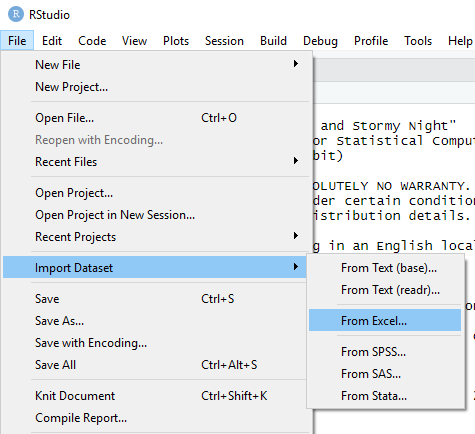
\includegraphics{images/importmenu.png}
\caption{R studio}
\end{figure}

\begin{enumerate}
\def\labelenumi{\arabic{enumi}.}
\setcounter{enumi}{1}
\tightlist
\item
  Belirli bir R komutunu kullanarak
\end{enumerate}

\begin{itemize}
\item
  İçe aktarmak istediğiniz dosyaya göz atın.
\item
  Veri seti için bir isim verin.
\item
  İçe aktarılacak sayfayı seçin.
\item
  Değişken isimleri dosyanın ilk satırındaysa ``First Row as Names''.
\end{itemize}

\begin{figure}
\centering
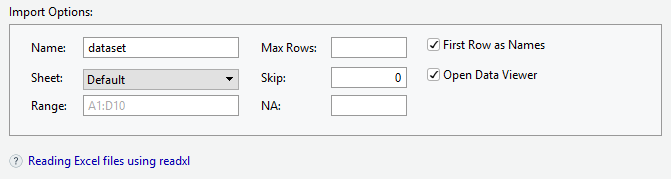
\includegraphics{images/excel1.png}
\caption{Excel dosylarını içe aktarma}
\end{figure}

\hypertarget{spss-dosylarux131nux131-iuxe7e-aktarma}{%
\subsection{SPSS dosylarını içe aktarma}\label{spss-dosylarux131nux131-iuxe7e-aktarma}}

\begin{itemize}
\item
  İçe aktarmak istediğiniz dosyaya göz atın.
\item
  Veri seti için bir isim verin.
\end{itemize}

\begin{figure}
\centering
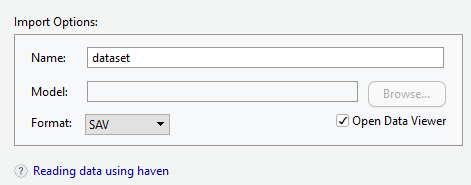
\includegraphics{images/spss1.png}
\caption{SPSS dosylarını içe aktarma}
\end{figure}

\hypertarget{veri-okuma}{%
\section{Veri Okuma}\label{veri-okuma}}

\begin{itemize}
\item
  En temel veri okuma/aktarma fonksiyonları

  \begin{itemize}
  \tightlist
  \item
    \texttt{scan()}
  \item
    \texttt{read.*}
  \item
    \texttt{read.table()}
  \item
    \texttt{read.csv()}
  \item
    \texttt{read.csv2()}
  \item
    \texttt{read.delim()}
  \item
    \texttt{read.delim2()}
  \item
    \texttt{readLines()}
  \end{itemize}
\item
  Verinin düzgün girilmiş olması okumayı kolaylaştırır.
\item
  İlk satırda genellikle değişken adlarına (header), ilk sütunda ise kimlik veya sıra numarasına yer verilir.
\item
  Gözlemlere ve değişkenlere ilişkin veri girilirken karakterler veya sayısal değerler arasında boşluk bırakmaktan kaçınmak gerekmektedir. Değişken adı boşluklu yazılmışsa ne olur?
\item
  Eksik veri boyunca aynı şekilde girilmelidir.
\item
  Değişkenlerin birinden nasıl ayrıldığı önemlidir. (, ; : ~/ )
\item
  Tercihimiz \textbf{.csv} uzantılı veriler ama büyük veri setleri az yer kalması icin \textbf{.txt,.prn} formatında karşımıza çıkabilmektedir.
\item
  Temel pakette \textbf{read.csv} ve \textbf{read.table} gibi bazı fonksiyonlar bulunmaktadır.
\item
  Ayrıca, belirli formatlarını içe aktarmak için R paketleri bulunmaktadır.Örneğin, SPSS dosyaları için \textbf{foreign} ve Excel dosyaları için \textbf{xlsx} gibi
\end{itemize}

\hypertarget{read.-fonksiyonlarux131}{%
\section{read.*() fonksiyonları}\label{read.-fonksiyonlarux131}}

\begin{longtable}[]{@{}
  >{\raggedright\arraybackslash}p{(\columnwidth - 2\tabcolsep) * \real{0.5000}}
  >{\raggedright\arraybackslash}p{(\columnwidth - 2\tabcolsep) * \real{0.5000}}@{}}
\toprule\noalign{}
\begin{minipage}[b]{\linewidth}\raggedright
\textbf{Argüman}
\end{minipage} & \begin{minipage}[b]{\linewidth}\raggedright
\textbf{Açıklama}
\end{minipage} \\
\midrule\noalign{}
\endhead
\bottomrule\noalign{}
\endlastfoot
\textbf{header} & Mantıksal değerler ile verinin ilk satırında değişken isimlerinin olup olmadığını test eder. \\
\textbf{sep} & Sütun ayracıdır. \\
\textbf{na.strings} & Kayıp değerleri belirtmek için kullanılır. \\
\textbf{dec} & Ondalık sayıların ne ile ayrıldığını gösteren argümandır. \\
\textbf{nrows} & Okunmak istenilen satır sayısını belirtmek için kullanılır. \\
\textbf{skip} & Bir dosya okunurken okunmadan atlanmak istenilen satır sayısı için kullanılır. \\
\end{longtable}

\hypertarget{excel-dosyasux131-aktarma}{%
\section{Excel dosyası aktarma}\label{excel-dosyasux131-aktarma}}

\begin{Shaded}
\begin{Highlighting}[]
\CommentTok{\# yükle ve aktive et }
\FunctionTok{install.packages}\NormalTok{(}\StringTok{"xlsx"}\NormalTok{)}
\FunctionTok{library}\NormalTok{(}\StringTok{"xlsx"}\NormalTok{)}

\CommentTok{\# read.xlsx fonksiyonunun kullanımı}
\NormalTok{my\_excel\_file }\OtherTok{\textless{}{-}} \FunctionTok{read.xlsx}\NormalTok{(}\StringTok{"dizin/dosyaadi.xlsx"}\NormalTok{,}\AttributeTok{sheetName =} \StringTok{"sheetname"}\NormalTok{)}
\end{Highlighting}
\end{Shaded}

\hypertarget{spss-dosyasux131-aktarma}{%
\subsection{SPSS dosyası aktarma}\label{spss-dosyasux131-aktarma}}

\begin{Shaded}
\begin{Highlighting}[]
\CommentTok{\# yükle ve aktive et }
\FunctionTok{install.packages}\NormalTok{(}\StringTok{"foreign"}\NormalTok{)}
\FunctionTok{library}\NormalTok{(}\StringTok{"foreign"}\NormalTok{)}

\CommentTok{\# read.spss fonksiyonunun kullanımı}
\NormalTok{my\_spss\_file }\OtherTok{\textless{}{-}} \FunctionTok{read.spss}\NormalTok{(}\StringTok{"dizin/dosyaadi.sav"}\NormalTok{,}
                \AttributeTok{to.data.frame =} \ConstantTok{TRUE}\NormalTok{)}
\end{Highlighting}
\end{Shaded}

\hypertarget{text-dosyasux131-aktarma}{%
\subsection{text dosyası aktarma}\label{text-dosyasux131-aktarma}}

\begin{itemize}
\tightlist
\item
  text dosyaları okumak için paket yüklemeye gerek yoktur.
\end{itemize}

\begin{Shaded}
\begin{Highlighting}[]
\CommentTok{\# , ile ayrılmış csv dosyaları}
\NormalTok{csv\_dosya }\OtherTok{\textless{}{-}} \FunctionTok{read.csv}\NormalTok{(}\StringTok{"dizin/dosyaadi.csv"}\NormalTok{,}\AttributeTok{header =} \ConstantTok{TRUE}\NormalTok{)}

\CommentTok{\# tab ile ayrılmış txt dosyaları}
\NormalTok{txt\_dosya }\OtherTok{\textless{}{-}} \FunctionTok{read.table}\NormalTok{(}\StringTok{"dizin/dosyaadi.txt"}\NormalTok{,}\AttributeTok{header =} \ConstantTok{TRUE}\NormalTok{, }\AttributeTok{sep =} \StringTok{"}\SpecialCharTok{\textbackslash{}t}\StringTok{"}\NormalTok{)}
\end{Highlighting}
\end{Shaded}

\begin{itemize}
\item
  Dikkat
\item
  \texttt{header\ =\ TRUE}
\item
  \texttt{sep="\textbackslash{}t"}
\item
  \texttt{sep=","} for comma-separated files
\item
\end{itemize}

\hypertarget{uygulama}{%
\section{Uygulama}\label{uygulama}}

\begin{itemize}
\item
  🔗Dosyaları buradan klasor halinde indirebilirsiniz. \href{import/import.rar}{DOSYALAR}
\item
  🔗\href{import/veri1.txt}{veri1.txt}
\end{itemize}

\begin{verbatim}
##    no m_1  m_2 m_3  m_4 m_5
## 1 522  12 14.0  16 20.0  10
## 2 222   5   NA  20 10.0  10
## 3 454   5 10.2   6  4.0  10
## 4 567  10 20.0  NA 12.2  20
\end{verbatim}

\begin{itemize}
\tightlist
\item
  🔗\href{import/veri1.csv}{veri1.csv}
\end{itemize}

\begin{verbatim}
##    no m_1  m_2 m_3  m_4 m_5
## 1 522  12 14.0  16 20.0  10
## 2 222   5   NA  20 10.0  10
## 3 454   5 10.2   6  4.0  10
## 4 567  10 20.0  NA 12.2  20
\end{verbatim}

\begin{itemize}
\tightlist
\item
\end{itemize}

\begin{verbatim}
##      No M1   M2 M3   M4 M5
## 001 522 12   14 16   20 10
## 002 222  5 <NA> 20   10 10
## 003 454  5 10,2  6    4 10
## 004 567 10   20 NA 12,2 20
\end{verbatim}

\begin{itemize}
\tightlist
\item
\end{itemize}

\begin{verbatim}
##     M1   M2 M3   M4 M5
## 001 12   14 16   20 10
## 002  5 <NA> 20   10 10
## 003  5 10,2  6    4 10
## 004 10   20 NA 12,2 20
\end{verbatim}

\begin{itemize}
\tightlist
\item
  🔗\href{import/fwf.txt}{verifwf.txt}
\item
\end{itemize}

\begin{verbatim}
##   V1  V2 V3 V4 V5 V6 V7 V8 V9 V10 V11 V12 V13
## 1  1 689  A  1  0  1  0  1  0   1   0   1   0
## 2  2 654  B  1  1  1  1  0  1   0   1   0   1
## 3  3 436  A  1  0  1  0  1  1   1   1   1   1
\end{verbatim}

\begin{itemize}
\tightlist
\item
\end{itemize}

\begin{verbatim}
##   sira  no kitapcik m1 m2 m3 m4 m5 m6 m7 m8 m9 m10
## 1    1 689        A  1  0  1  0  1  0  1  0  1   0
## 2    2 654        B  1  1  1  1  0  1  0  1  0   1
## 3    3 436        A  1  0  1  0  1  1  1  1  1   1
\end{verbatim}

\begin{itemize}
\tightlist
\item
  🔗\href{import/factor.sav}{factor.sav}
\end{itemize}

\begin{verbatim}
## tibble [50 x 3] (S3: tbl_df/tbl/data.frame)
##  $ id   : num [1:50] 1 2 3 4 5 6 7 8 9 10 ...
##   ..- attr(*, "format.spss")= chr "F6.2"
##  $ bolge: num [1:50] 1 1 1 1 1 1 1 1 1 1 ...
##   ..- attr(*, "format.spss")= chr "F6.2"
##  $ puan : num [1:50] 9 8 6 8 10 4 6 5 7 7 ...
##   ..- attr(*, "format.spss")= chr "F6.2"
\end{verbatim}

\begin{itemize}
\tightlist
\item
  🔗 \url{https://www.statmodel.com/usersguide/chap3/ex3.1.dat}
\end{itemize}

\begin{verbatim}
##  [1] -0.354517  0.561655  0.315551  3.347049 -0.122389 -0.251276 -0.517996
##  [8]  1.888854  0.461254  2.237483
\end{verbatim}

\begin{itemize}
\tightlist
\item
\end{itemize}

\begin{verbatim}
##  [1] "   -0.354517     0.573051    -0.175230"
##  [2] "    0.561655    -0.368095     1.090042"
##  [3] "    0.315551    -0.577052     0.425472"
##  [4] "    3.347049     1.088520     1.149353"
##  [5] "   -0.122389    -0.694153    -0.766538"
##  [6] "   -0.251276    -0.017487    -1.367410"
##  [7] "   -0.517996    -0.817974    -1.559255"
##  [8] "    1.888854    -0.658335     1.007614"
##  [9] "    0.461254     0.463916    -0.898300"
## [10] "    2.237483     1.533398     0.180512"
\end{verbatim}

\hypertarget{veri-yazma}{%
\section{Veri Yazma}\label{veri-yazma}}

\begin{Shaded}
\begin{Highlighting}[]
\NormalTok{ad  }\OtherTok{\textless{}{-}}  \FunctionTok{c}\NormalTok{(}\StringTok{"Ali"}\NormalTok{,}\StringTok{"Elif"}\NormalTok{,}\StringTok{"Su"}\NormalTok{,}\StringTok{"Deniz"}\NormalTok{,}\StringTok{"Aras"}\NormalTok{,}\StringTok{"Berk"}\NormalTok{,}\StringTok{"Can"}\NormalTok{,}\StringTok{"Ece"}\NormalTok{,}\StringTok{"Efe"}\NormalTok{,}\StringTok{"Arda"}\NormalTok{)}
\NormalTok{boy }\OtherTok{\textless{}{-}} \FunctionTok{c}\NormalTok{(}\DecValTok{160}\NormalTok{,}\DecValTok{165}\NormalTok{,}\DecValTok{170}\NormalTok{,}\DecValTok{155}\NormalTok{,}\DecValTok{167}\NormalTok{,}\DecValTok{162}\NormalTok{,}\DecValTok{169}\NormalTok{,}\DecValTok{158}\NormalTok{,}\DecValTok{160}\NormalTok{,}\DecValTok{164}\NormalTok{)}
\NormalTok{kilo }\OtherTok{\textless{}{-}} \FunctionTok{c}\NormalTok{(}\DecValTok{50}\NormalTok{,}\DecValTok{55}\NormalTok{,}\DecValTok{57}\NormalTok{,}\DecValTok{50}\NormalTok{,}\DecValTok{48}\NormalTok{,}\DecValTok{65}\NormalTok{,}\DecValTok{58}\NormalTok{,}\DecValTok{62}\NormalTok{,}\DecValTok{45}\NormalTok{,}\DecValTok{47}\NormalTok{)}
\NormalTok{beden }\OtherTok{\textless{}{-}} \FunctionTok{c}\NormalTok{(}\StringTok{"S"}\NormalTok{,}\StringTok{"M"}\NormalTok{,}\StringTok{"S"}\NormalTok{,}\StringTok{"M"}\NormalTok{,}\StringTok{"S"}\NormalTok{,}\StringTok{"L"}\NormalTok{,}\StringTok{"M"}\NormalTok{,}\StringTok{"L"}\NormalTok{,}\StringTok{"S"}\NormalTok{,}\StringTok{"S"}\NormalTok{)}
\NormalTok{df }\OtherTok{\textless{}{-}} \FunctionTok{data.frame}\NormalTok{(ad, boy, kilo, beden)}
\NormalTok{df}
\end{Highlighting}
\end{Shaded}

\begin{verbatim}
##       ad boy kilo beden
## 1    Ali 160   50     S
## 2   Elif 165   55     M
## 3     Su 170   57     S
## 4  Deniz 155   50     M
## 5   Aras 167   48     S
## 6   Berk 162   65     L
## 7    Can 169   58     M
## 8    Ece 158   62     L
## 9    Efe 160   45     S
## 10  Arda 164   47     S
\end{verbatim}

\begin{Shaded}
\begin{Highlighting}[]
\FunctionTok{write.table}\NormalTok{(df, }\AttributeTok{file=}\StringTok{"df.txt"}\NormalTok{)}\CommentTok{\# df dosyasi nerede, gorunumu nasil}
\end{Highlighting}
\end{Shaded}

\begin{Shaded}
\begin{Highlighting}[]
\FunctionTok{write.table}\NormalTok{(df, }\AttributeTok{file=}\StringTok{"df.txt"}\NormalTok{,}\AttributeTok{row.names =} \ConstantTok{FALSE}\NormalTok{,}\AttributeTok{col.names =} \ConstantTok{FALSE}\NormalTok{)}
\CommentTok{\# karakter nesnler tirnak icinde ne yapmali?}
\end{Highlighting}
\end{Shaded}

\begin{Shaded}
\begin{Highlighting}[]
\FunctionTok{write.table}\NormalTok{(df, }\AttributeTok{file=}\StringTok{"df.txt"}\NormalTok{,}\AttributeTok{row.names =} \ConstantTok{FALSE}\NormalTok{,}\AttributeTok{col.names =} \ConstantTok{FALSE}\NormalTok{,}\AttributeTok{quote=}\ConstantTok{FALSE}\NormalTok{)}
\end{Highlighting}
\end{Shaded}

yeni gözlem eklemek istiyorsaniz append argümanı kullanılabilir.

\begin{Shaded}
\begin{Highlighting}[]
\NormalTok{ ek }\OtherTok{\textless{}{-}} \FunctionTok{data.frame}\NormalTok{(}\AttributeTok{ad=}\FunctionTok{c}\NormalTok{(}\StringTok{"Ahmet"}\NormalTok{,}\StringTok{"Ali"}\NormalTok{), }\AttributeTok{boy=}\FunctionTok{c}\NormalTok{(}\DecValTok{180}\NormalTok{,}\DecValTok{170}\NormalTok{), }\AttributeTok{kilo=}\FunctionTok{c}\NormalTok{(}\DecValTok{60}\NormalTok{,}\DecValTok{70}\NormalTok{), }
                 \AttributeTok{beden=}\FunctionTok{c}\NormalTok{(}\StringTok{"S"}\NormalTok{,}\StringTok{"L"}\NormalTok{))}
\end{Highlighting}
\end{Shaded}

\begin{Shaded}
\begin{Highlighting}[]
\FunctionTok{write.table}\NormalTok{(ek, }\StringTok{"df.txt"}\NormalTok{,}\AttributeTok{row.names=}\ConstantTok{FALSE}\NormalTok{,}
            \AttributeTok{col.names=}\ConstantTok{FALSE}\NormalTok{,}
            \AttributeTok{quote=}\ConstantTok{FALSE}\NormalTok{,}\AttributeTok{append=}\ConstantTok{TRUE}\NormalTok{)}
\end{Highlighting}
\end{Shaded}

\begin{itemize}
\item
  \textbf{write.csv()} fonksiyonu kullanılarak yazılan veri dosyaları ``,'' ile,
\item
  \textbf{write.csv2()} fonksiyonu kullanılarak yazılan veri dosyaları ise ``;'' ile ayrılır iki fonksiyonun bir diğer farkı ise ondalık sayı ayıracıdır.
\item
  write.csv ile yazdırılan dosyaların excelde açılması
\end{itemize}

\hypertarget{cat-fonksiyonu}{%
\subsection{\texorpdfstring{\textbf{cat()} fonksiyonu}{cat() fonksiyonu}}\label{cat-fonksiyonu}}

\begin{itemize}
\tightlist
\item
  Döngülerde sıklıkla ekrana bilgi yazdırmak amacıyla kullanılır, ancak dosya yazdırmak amacıyla da kullanabilmektedir.
\item
  fonksiyonlarla yapılan hesaplama çıktısı da yazabilmektedir.
\item
  Bu nedenle bir R oturumu sırasında not alınmak istenilen bilgileri bir dosyaya yazdırmak için kullanılabilir.
\end{itemize}

\begin{Shaded}
\begin{Highlighting}[]
 \FunctionTok{cat}\NormalTok{(}\StringTok{"ogrencilerin boy ortalamasi "}\NormalTok{, }\FunctionTok{mean}\NormalTok{(boy), }\StringTok{"}\SpecialCharTok{\textbackslash{}n}\StringTok{"}\NormalTok{,}
      \StringTok{"ogrencilerin kilo ortalamasi"}\NormalTok{, }\FunctionTok{mean}\NormalTok{(kilo), }\StringTok{"}\SpecialCharTok{\textbackslash{}n}\StringTok{"}\NormalTok{,}
     \AttributeTok{file=}\StringTok{"bilgi.txt"}\NormalTok{)}
\end{Highlighting}
\end{Shaded}

\begin{itemize}
\tightlist
\item
  \n ne ise yaradi?
\end{itemize}

\hypertarget{writelines-fonksiyonu}{%
\section{writeLines fonksiyonu}\label{writelines-fonksiyonu}}

\begin{Shaded}
\begin{Highlighting}[]
\FunctionTok{writeLines}\NormalTok{(}\StringTok{"ogrencilerin boy ortalamasi: 163 cm}\SpecialCharTok{\textbackslash{}n}\StringTok{"}\NormalTok{,}
            \StringTok{"ogrencilerin kilo ortalamasi: 53.7 kg"}\NormalTok{,}
            \AttributeTok{con=}\StringTok{"bilgi2.txt"}\NormalTok{)}
\end{Highlighting}
\end{Shaded}

\hypertarget{odev-2}{%
\section{ODEV}\label{odev-2}}

\begin{itemize}
\item
  🔗 \href{https://psyteachr.github.io/data-skills-v1/getting-to-know-the-data.html}{Linkte} yer alan sayfayı inceleyiniz. Bu sayfada bir veri setini incelemeniz ve bu veri seti ile ilgili sorulara cevap vermeniz beklenemketedir.
\item
  🔗\href{https://psyteachr.github.io/data-skills-v1/loading-data.html}{Linkte} yer alan sayfada sizden iki veri setini okumanız beklenmeketdir. Bu iki veri setini okuduktan sonra da hazır kodları incelemeniz ve bu kodlar ile ilgili sorulara cevap vermeniz beklenmektedir.
\end{itemize}

☕

\hypertarget{veri-duzenleme---i}{%
\chapter{Veri duzenleme - I}\label{veri-duzenleme---i}}

\hypertarget{dplyr-paket-tanux131tux131mux131}{%
\section{dplyr paket tanıtımı}\label{dplyr-paket-tanux131tux131mux131}}

\begin{itemize}
\item
  Veri düzenlemede en sık kullanılan paketlerden biri \textbf{dplyr} paketidir.
\item
  Veri manipulasyonunun \texttt{grammeri} paketin tanıtımında kullanılmıştır.
\item
  Paketin en sık kullanılan fonksiyonları ise

  \begin{itemize}
  \item
    \texttt{select():} istenilen değişkenlere gore yeni bir veri seti oluşturma
  \item
    \texttt{mutate():} yeni degişkenlerin veri setine eklenmesi
  \item
    \texttt{filter():} istenilen gözlemlerle yeni bir veri oluşturma
  \item
    \texttt{arrange():} gözlemlerin seçilen degişkenlere göre yeniden sıralanması
  \item
    \texttt{group\_by():} veride grup bazinda işlem yapma
  \item
    \texttt{summarise():} veriden özet istatisikleri elde etme
  \item
    \texttt{baglama\ (pipe)} \texttt{\%\textgreater{}\%} - işlemleri bağlama
  \item
    \texttt{join()} - veri birleştirme
  \end{itemize}
\end{itemize}

\hypertarget{paket-vignetteleri}{%
\section{Paket vignetteleri 📊}\label{paket-vignetteleri}}

\begin{itemize}
\item
  🔗 \href{https://cran.r-project.org/web/packages/dplyr/vignettes/base.html}{From base R to dplyr}
\item
  🔗 \href{https://cran.r-project.org/web/packages/dplyr/vignettes/colwise.html}{colwise}
\item
  🔗 \href{https://cran.r-project.org/web/packages/dplyr/vignettes/compatibility.html}{dplyr compatibility}
\item
  🔗 \href{https://cran.r-project.org/web/packages/dplyr/vignettes/dplyr.html}{Introduction to dplyr}
\item
  🔗 \href{https://cran.r-project.org/web/packages/dplyr/vignettes/grouping.html}{Grouped data}
\item
  🔗 \href{https://cran.r-project.org/web/packages/dplyr/vignettes/programming.html}{Programming with dplyr}
\item
  🔗 \href{https://cran.r-project.org/web/packages/dplyr/vignettes/rowwise.html}{rowwise}
\item
  🔗 \href{https://cran.r-project.org/web/packages/dplyr/vignettes/two-table.html}{Two-table verbs}
\item
  🔗 \href{https://cran.r-project.org/web/packages/dplyr/vignettes/window-functions.html}{Window functions}
\item
  🔗 paketin cran sayfası \href{https://cran.r-project.org/web/packages/dplyr/index.html}{link}
\item
  🔗 paketin indirilme istatistikleri \href{https://ipub.com/dev-corner/apps/r-package-downloads/}{link}
\end{itemize}

\hypertarget{uluslararasux131-eux11fitim-araux15ftux131rmalarux131}{%
\section{Uluslararası Eğitim Araştırmaları}\label{uluslararasux131-eux11fitim-araux15ftux131rmalarux131}}

\hypertarget{pisa}{%
\subsection{PISA}\label{pisa}}

\begin{itemize}
\item
  Program for International Student Assessment-PISA (Uluslararası Öğrenci Değerlendirme Programı)
\item
  15 yaş grubundaki öğrencilerin matematik, fen ve okuma
  becerilerindeki durumlarını belirlemeye yönelik bir çalışmadır.
\item
  Ekonomik İşbirliği ve Kalkınma Örgütü (OECD) tarafından düzenlenir.
\end{itemize}

\hypertarget{timss}{%
\subsection{TIMSS}\label{timss}}

\begin{itemize}
\item
  Trends in International Mathematics and Science Study (Uluslararası Matematik ve Fen Eğilimleri Araştırması)
\item
  Öğrencilerin matematik ve fen alanlarında kazandıkları bilgi ve becerilerin değerlendirilmesine yönelik bir tarama araştırmasıdır.
\item
  Uluslararası Eğitim Başarılarını Değerlendirme Kuruluşu'nun bir projesidir.
\end{itemize}

\hypertarget{veri-setleri-1}{%
\section{Veri Setleri}\label{veri-setleri-1}}

\begin{itemize}
\item
  🔗 \href{https://www.oecd.org/pisa/data/}{PISA database}
\item
  🔗 \href{https://timss2019.org/international-database/}{TIMSS 2019 database}
\item
  🔗 \href{https://timssandpirls.bc.edu/timss2015/international-database/}{TIMSS 2015 database}
\item
  🔗 \href{https://timssandpirls.bc.edu/timss2011/international-database.html}{TIMSS 2015 database}
\end{itemize}

\hypertarget{uluslararasux131-sux131navlarla-ilgili-r-paketleri}{%
\section{Uluslararası Sınavlarla İlgili R paketleri}\label{uluslararasux131-sux131navlarla-ilgili-r-paketleri}}

\hypertarget{instvy-paketi-international-assessment-data-manager}{%
\subsection{\texorpdfstring{\textbf{instvy} paketi: International Assessment Data Manager}{instvy paketi: International Assessment Data Manager}}\label{instvy-paketi-international-assessment-data-manager}}

\begin{itemize}
\item
  \textbf{intsvy} paketi (Caro ve Biecek, 2017) TIMSS, PIRLS, PISA ve ICILS gibi uluslararası değerlendirme çalışmalarının verilerini aktarma, birleştirme ve analiz etme amacıyla geliştirilmiştir.
\item
  \textbf{intsvy} paketindeki \textbf{pisa.select.merge()} fonksiyonuyla aşağıdaki komutlar kullanılarak istenilen ülke/ülkelerin istenilen değişkenlerine ilişkin veri seti oluşturulabilir.
\item
  İlgili fonksiyon bir SPSS dosyası okuduğu için \textbf{.sav} uzantılı dosyaların okunmasında kullanılan \textbf{foreign} paketi sistemde yüklü olmalıdır.
\item
  Türkiye öğrenci anketi veri dosyasında yer alan sekiz ve Türkiye okul anketi veri dosyasında yer alan üç değişken seçilerek ve ``pisa2015'' nesnesi oluşturmuştur.
\end{itemize}

\begin{Shaded}
\begin{Highlighting}[]
\FunctionTok{library}\NormalTok{(}\StringTok{"intsvy"}\NormalTok{)}
\FunctionTok{library}\NormalTok{(}\StringTok{"foreign"}\NormalTok{)}
\NormalTok{pisa2015 }\OtherTok{\textless{}{-}} \FunctionTok{pisa.select.merge}\NormalTok{(}\AttributeTok{folder=}\StringTok{"F:}\SpecialCharTok{\textbackslash{}\textbackslash{}}\StringTok{PISA"}\NormalTok{, }\CommentTok{\# folder=getwd()}
\AttributeTok{student.file=}\StringTok{"CY6\_MS\_CMB\_STU\_QQQ.sav"}\NormalTok{,}
\AttributeTok{school.file=}\StringTok{"CY6\_MS\_CMB\_SCH\_QQQ.sav"}\NormalTok{,}
\AttributeTok{student=}\FunctionTok{c}\NormalTok{(}\StringTok{"ST001D01T"}\NormalTok{,}\StringTok{"ST004D01T"}\NormalTok{,}\StringTok{"STRATUM"}\NormalTok{,}\StringTok{"MISCED"}\NormalTok{,}\StringTok{"FISCED"}\NormalTok{,}\StringTok{"IMMIG"}\NormalTok{,}\StringTok{"LANGN"}\NormalTok{,}\StringTok{"ESCS"}\NormalTok{,)}
\AttributeTok{school=}\FunctionTok{c}\NormalTok{(}\StringTok{"SCHSIZE"}\NormalTok{,}\StringTok{"CLSIZE"}\NormalTok{,}\StringTok{"STRATIO"}\NormalTok{),}
  \AttributeTok{countries=}\FunctionTok{c}\NormalTok{(}\StringTok{"TUR"}\NormalTok{))}
\end{Highlighting}
\end{Shaded}

Komutların çalısması uzun zaman alabilir. Büyük dosyaların okunması sırasında, dosya büyüklüğüne ve bilgisayar özelliklerine bağlı olarak, mevcut \textbf{bellek (memory)} hata mesajı alınabilir.

\hypertarget{edsurvey-paketi}{%
\subsection{\texorpdfstring{\textbf{EdSurvey} paketi}{EdSurvey paketi}}\label{edsurvey-paketi}}

\begin{itemize}
\tightlist
\item
  PISA, TALIS, PIAAC, TIMSS, PIRLS, ICILS gibi sınavların veri setlerini indirmede, karmaşık veri setlerini \textbf{olası puanları} dikkate alarak analiz etmede kullanılan bir pakettir.
\end{itemize}

\begin{Shaded}
\begin{Highlighting}[]
\FunctionTok{library}\NormalTok{(EdSurvey)}
\end{Highlighting}
\end{Shaded}

\begin{itemize}
\tightlist
\item
  Örnek olarak aşağıda yer alan kod 2012 yılı PISA veri setini, bilgisayarınızda istediğiniz yere indirecektir.
\end{itemize}

\begin{Shaded}
\begin{Highlighting}[]
\FunctionTok{downloadPISA}\NormalTok{(}\AttributeTok{years =} \DecValTok{2012}\NormalTok{, }\AttributeTok{database =} \FunctionTok{c}\NormalTok{(}\StringTok{"INT"}\NormalTok{), }\AttributeTok{root=}\FunctionTok{getwd}\NormalTok{())}
\end{Highlighting}
\end{Shaded}

\begin{itemize}
\item
  bu işlem de bilgisayar özelliklerine bağlı da olsa \textbf{zaman alan} bir işlemdir.
\item
  Aşağıdaki kod sgp olarak kodlu olan Singapur ülkesine ilişkin verileri çeker.
\end{itemize}

\begin{Shaded}
\begin{Highlighting}[]
\NormalTok{sgp2012 }\OtherTok{\textless{}{-}} \FunctionTok{readPISA}\NormalTok{(}\AttributeTok{path =} \StringTok{"sunum/PISA/2012"}\NormalTok{, }\AttributeTok{database =} \StringTok{"INT"}\NormalTok{, }\AttributeTok{countries =} \StringTok{"sgp"}\NormalTok{)}
\end{Highlighting}
\end{Shaded}

\begin{itemize}
\item
  bu işlem de bilgisayar özelliklerine bağlı da olsa zaman alan bir işlemdir.
\item
  Bu tarz uzun süren işlemleri tekrarlamamak için, oluşan veriyi daha sonra R ortamına kolayca aktarmak için \textbf{saveRDS()} fonkisyonu ile \textbf{.Rds}, \textbf{save()} ile \textbf{.Rdata} bir dosyaya kaydedebilirsiniz.
\item
  Oluşan dosya tekrar R ortamına \textbf{readRDS()} ya da \textbf{load()} fonksiyonu ile aktarılabilir.
\item
  Oluşan sgp2012 verisinden istediğiniz sütunları \textbf{getData()} fonksiyonu ile seçebilirsiniz.
\end{itemize}

\begin{Shaded}
\begin{Highlighting}[]
\CommentTok{\# okuma ve agirlandirma degiskenlerini gg nesnesine atama}
\NormalTok{gg }\OtherTok{\textless{}{-}}\NormalTok{ EdSurvey}\SpecialCharTok{::}\FunctionTok{getData}\NormalTok{(sgp2012, }\FunctionTok{c}\NormalTok{(}\StringTok{"cnt"}\NormalTok{,}\StringTok{"read"}\NormalTok{,}\StringTok{"w\_fstuwt"}\NormalTok{))  }
\FunctionTok{head}\NormalTok{(gg)}
\end{Highlighting}
\end{Shaded}

\begin{Shaded}
\begin{Highlighting}[]
\FunctionTok{edsurveyTable}\NormalTok{(read }\SpecialCharTok{\textasciitilde{}}\NormalTok{ st04q01 }\SpecialCharTok{+}\NormalTok{ st20q01, }\AttributeTok{data =}\NormalTok{ sgp2012)}
\end{Highlighting}
\end{Shaded}

\hypertarget{ralsa}{%
\subsection{RALSA}\label{ralsa}}

\begin{itemize}
\item
  🔗 \href{http://ralsa.ineri.org/user-guide/}{RALSA}
\item
  The R Analyzer for Large-Scale Assessments (RALSA)
\end{itemize}

\begin{Shaded}
\begin{Highlighting}[]
\FunctionTok{library}\NormalTok{(RALSA)}
\end{Highlighting}
\end{Shaded}

\hypertarget{olasux131-deux11fer}{%
\section{Olası Değer}\label{olasux131-deux11fer}}

\begin{itemize}
\item
  450 kişilik bir grupta 150 kadın 300 erkek olduğu bir evrenden 60 kişinin oluşturduğu bir örneklemin rastgele seçildiğini düşünelim.
\item
  Bu seçim sonucu 30 kadın 30 erkek seçilmiş olsun.
\item
  Evrende erkekler kadınlardan daha çok temsil edilirken örneklemde eşit temsil edilmektedirler.
\item
  Kadınların örnekleme seçilme olasılığı = 30/150=0.2
\item
  Erkeklerin örnekleme seçilme olasılığı = 30/300=0.1
\item
  örnekleme ilişkin ölçümler
\end{itemize}

\begin{Shaded}
\begin{Highlighting}[]
\FunctionTok{set.seed}\NormalTok{(}\DecValTok{41}\NormalTok{)}
\NormalTok{kadin }\OtherTok{\textless{}{-}} \FunctionTok{sample}\NormalTok{(}\DecValTok{50}\SpecialCharTok{:}\DecValTok{90}\NormalTok{,}\DecValTok{30}\NormalTok{)}
\NormalTok{erkek }\OtherTok{\textless{}{-}} \FunctionTok{sample}\NormalTok{(}\DecValTok{30}\SpecialCharTok{:}\DecValTok{70}\NormalTok{,}\DecValTok{30}\NormalTok{)}

\NormalTok{kadin}
\end{Highlighting}
\end{Shaded}

\begin{verbatim}
##  [1] 89 84 54 81 57 78 55 71 80 62 87 67 70 83 82 61 66 53 50 69 79 64 85 51 73
## [26] 74 88 52 72 90
\end{verbatim}

\begin{Shaded}
\begin{Highlighting}[]
\NormalTok{erkek}
\end{Highlighting}
\end{Shaded}

\begin{verbatim}
##  [1] 45 56 57 39 37 42 47 50 68 49 62 63 58 69 31 59 52 64 65 66 55 48 30 33 46
## [26] 53 51 67 40 41
\end{verbatim}

\begin{Shaded}
\begin{Highlighting}[]
\FunctionTok{mean}\NormalTok{(kadin)}
\end{Highlighting}
\end{Shaded}

\begin{verbatim}
## [1] 70.9
\end{verbatim}

\begin{Shaded}
\begin{Highlighting}[]
\FunctionTok{mean}\NormalTok{(erkek)}
\end{Highlighting}
\end{Shaded}

\begin{verbatim}
## [1] 51.43333
\end{verbatim}

\begin{itemize}
\tightlist
\item
  örneklem ağırlıklandırılması \textbf{kullanılmadan} ortalama
\end{itemize}

\begin{Shaded}
\begin{Highlighting}[]
\NormalTok{(}\FunctionTok{sum}\NormalTok{(kadin)}\SpecialCharTok{+}\FunctionTok{sum}\NormalTok{(erkek))}\SpecialCharTok{/}\DecValTok{60}
\end{Highlighting}
\end{Shaded}

\begin{verbatim}
## [1] 61.16667
\end{verbatim}

\begin{itemize}
\tightlist
\item
  örneklem ağırlıklandırılması \textbf{kullanılarak} ortalama
\end{itemize}

\begin{Shaded}
\begin{Highlighting}[]
\NormalTok{(}\FunctionTok{sum}\NormalTok{(kadin)}\SpecialCharTok{*}\NormalTok{(}\DecValTok{1}\SpecialCharTok{/}\FloatTok{0.2}\NormalTok{) }\SpecialCharTok{+} \FunctionTok{sum}\NormalTok{(erkek)}\SpecialCharTok{*}\NormalTok{(}\DecValTok{1}\SpecialCharTok{/}\FloatTok{0.1}\NormalTok{))}\SpecialCharTok{/}\DecValTok{450}
\end{Highlighting}
\end{Shaded}

\begin{verbatim}
## [1] 57.92222
\end{verbatim}

\hypertarget{tuxfcrkiye-veri-setleri}{%
\section{Türkiye Veri Setleri}\label{tuxfcrkiye-veri-setleri}}

\begin{itemize}
\item
  Türkiye Uluslararası Eğitim Verisi \textbf{(tuev)} geniş kapsamlı uluslararası başarı değerlendirme programlarından \textbf{PISA} ve \textbf{TIMSS} Türkiye verilerini depolayan bir R kütüphanesidir.
\item
  Bu eğitimde

  \begin{itemize}
  \tightlist
  \item
    \textbf{PISA 2018} (OECD, 2019) \\
  \item
    \textbf{TIMSS 2019} (Mullis, Martin, Foy, Kelly, \& Fishbein; 2020) \\
    veri setleri kullanılacaktır.
  \end{itemize}
\end{itemize}

\hypertarget{tuev-paketin-yuxfcklenmesi}{%
\section{\texorpdfstring{\textbf{tuev} paketin yüklenmesi}{tuev paketin yüklenmesi}}\label{tuev-paketin-yuxfcklenmesi}}

\begin{itemize}
\tightlist
\item
  githubdan paket yükleyebilmek için yüklenmesi gereken paket 📦
\end{itemize}

\begin{Shaded}
\begin{Highlighting}[]
\FunctionTok{install.packages}\NormalTok{(}\StringTok{"devtools"}\NormalTok{)}
\CommentTok{\# devtools paketinin etkinleştirilmesi}
\FunctionTok{library}\NormalTok{(devtools)}
\end{Highlighting}
\end{Shaded}

\begin{itemize}
\tightlist
\item
  tuev paketinin yüklenmesi 📦
\end{itemize}

\begin{Shaded}
\begin{Highlighting}[]
\NormalTok{devtools}\SpecialCharTok{::}\FunctionTok{install\_github}\NormalTok{(}\StringTok{"tuevpaket/tuev"}\NormalTok{)}
\CommentTok{\#paketin etkinleştirilmesi}
\FunctionTok{library}\NormalTok{(tuev)}
\end{Highlighting}
\end{Shaded}

\begin{itemize}
\tightlist
\item
\end{itemize}

\hypertarget{pisa-2018-verisi}{%
\section{PISA 2018 Verisi}\label{pisa-2018-verisi}}

\begin{itemize}
\tightlist
\item
  bilissel veri seti
\end{itemize}

\begin{Shaded}
\begin{Highlighting}[]
\FunctionTok{load}\NormalTok{(}\StringTok{"import/PISA\_COG\_2018.rda"}\NormalTok{)}
\end{Highlighting}
\end{Shaded}

\begin{itemize}
\tightlist
\item
  ogrenci veri seti
\end{itemize}

\begin{Shaded}
\begin{Highlighting}[]
\FunctionTok{load}\NormalTok{(}\StringTok{"import/PISA\_STU\_2018.rda"}\NormalTok{) }\CommentTok{\# ogrenci verisi}
\end{Highlighting}
\end{Shaded}

\begin{itemize}
\tightlist
\item
  okul veri seti
\end{itemize}

\begin{Shaded}
\begin{Highlighting}[]
\FunctionTok{load}\NormalTok{(}\StringTok{"import/PISA\_SCH\_2018.rda"}\NormalTok{) }\CommentTok{\# okul verisi}
\end{Highlighting}
\end{Shaded}

\hypertarget{pipe}{%
\section{\texorpdfstring{pipe \textbf{\%\textgreater\%}}{pipe \%\textgreater\%}}\label{pipe}}

\begin{itemize}
\item
  \textbf{dplyr()} paketindeki tüm fonksiyonlar daha az değişken oluşturmak amacıyla pipe operatorü \textbf{\%\textgreater\%} ile kullanılabilir.
\item
  \textbf{\%\textgreater\%} operatorü sık kullanılan bir operatördür.
\item
  kısa yolu: \textbf{Ctrl+Shift+M}
\item
  kısa yolu(mac) :\textbf{Cmd + Shift + M}
\item
  \textbf{\%\textgreater\%} operatorün yer aldığı paket ise \textbf{magrittr}
\end{itemize}

\begin{Shaded}
\begin{Highlighting}[]
\FunctionTok{library}\NormalTok{(magrittr)}
\end{Highlighting}
\end{Shaded}

\begin{itemize}
\tightlist
\item
  \textbf{\%\textgreater\%} solundaki nesneye sağındaki fonksiyonu uygular.
\end{itemize}

\begin{Shaded}
\begin{Highlighting}[]
\NormalTok{x }\SpecialCharTok{\%\textgreater{}\%} \FunctionTok{f}\NormalTok{(y) }\OtherTok{=} \FunctionTok{f}\NormalTok{(x, y)}
\end{Highlighting}
\end{Shaded}

\begin{itemize}
\tightlist
\item
  \textbf{\%\textgreater\%} 👉
\end{itemize}

\begin{Shaded}
\begin{Highlighting}[]
\FunctionTok{library}\NormalTok{(gapminder)}
\NormalTok{gapminder }\SpecialCharTok{\%\textgreater{}\%}
  \FunctionTok{filter}\NormalTok{(country }\SpecialCharTok{==} \StringTok{"Canada"}\NormalTok{) }\SpecialCharTok{\%\textgreater{}\%}
  \FunctionTok{head}\NormalTok{(}\DecValTok{2}\NormalTok{)}
\end{Highlighting}
\end{Shaded}

\begin{verbatim}
## # A tibble: 2 x 6
##   country continent  year lifeExp      pop gdpPercap
##   <fct>   <fct>     <int>   <dbl>    <int>     <dbl>
## 1 Canada  Americas   1952    68.8 14785584    11367.
## 2 Canada  Americas   1957    70.0 17010154    12490.
\end{verbatim}

\begin{itemize}
\item
  bizi fazla yazmaktan kurtarır.
\item
  kodu okunabilir kılar.
\item
  zincirlemeye/bağlamaya izin verir.
\item
  Veri düzenleme işlerinde her zaman kullanışlıdır.
\item
  pipe, her bir fonksiyonu ayrı bir satırda bulundurduğunuzda en net şekilde okunur.
\end{itemize}

\begin{Shaded}
\begin{Highlighting}[]
\NormalTok{veri }\SpecialCharTok{\%\textgreater{}\%}
  \FunctionTok{ilk\_fonksiyon}\NormalTok{(.....) }\SpecialCharTok{\%\textgreater{}\%}
  \FunctionTok{ikinci\_fonksiyon}\NormalTok{(.....) }\SpecialCharTok{\%\textgreater{}\%}
  \FunctionTok{ucuncu\_fonksiyon}\NormalTok{(.....) }\SpecialCharTok{\%\textgreater{}\%}\NormalTok{ ...}
\end{Highlighting}
\end{Shaded}

\begin{itemize}
\item
  pipenin solundaki öğeler, sağdaki fonksiyonun ilk argümanına iletilir.
\item
  Fonksiyon ilk argümanı olan veriyi pipenin \textbf{solundan} alır, kalan argümanlar fonksiyonun \textbf{sağındadır.}
\item
  Bazı fonksiyonların, ilk argümanı veri seti olmayabilir. Bu durumda veri seti argüman değeri \textbf{.} olarak kullanılabilir.
\item
  Veri seti regresyon modelinde ilk argüman değildir.
\end{itemize}

\begin{Shaded}
\begin{Highlighting}[]
\NormalTok{veri }\SpecialCharTok{\%\textgreater{}\%} \FunctionTok{lm}\NormalTok{(degisken1 }\SpecialCharTok{\textasciitilde{}}\NormalTok{ degisken2, }\AttributeTok{data=}\NormalTok{ .)}
\end{Highlighting}
\end{Shaded}

\begin{itemize}
\tightlist
\item
  pipe kullanımı ile oluşan çıktıdan yeni bir nesne oluşturmak istiyorsanız, atama operatorü \textbf{\textless-}
  kullanmalısınız 🔗.
\end{itemize}

\begin{Shaded}
\begin{Highlighting}[]
\NormalTok{yeninesne }\OtherTok{\textless{}{-}}\NormalTok{ veri }\SpecialCharTok{\%\textgreater{}\%} \FunctionTok{lm}\NormalTok{(degisken1 }\SpecialCharTok{\textasciitilde{}}\NormalTok{ degisken2, }\AttributeTok{data=}\NormalTok{ .)}
\end{Highlighting}
\end{Shaded}

Bağlama işlemleri ne kadar uzun olursa olsun \textbf{\textless-} operatorü en başta olmalıdır.

\begin{itemize}
\tightlist
\item
  Veri setlerinde yapı incelemek için \textbf{glimpse()}, \textbf{str()} gibi fonksiyonlar kullanılabilir.
\end{itemize}

\begin{Shaded}
\begin{Highlighting}[]
\FunctionTok{glimpse}\NormalTok{(PISA\_COG\_2018)}
\end{Highlighting}
\end{Shaded}

\begin{itemize}
\tightlist
\item
  Veri setlerinde yapı incelemek için \textbf{glimpse()}, \textbf{str()} gibi fonksiyonlar kullanılabilir.
\end{itemize}

\begin{Shaded}
\begin{Highlighting}[]
\FunctionTok{glimpse}\NormalTok{(PISA\_STU\_2018)}
\end{Highlighting}
\end{Shaded}

\begin{Shaded}
\begin{Highlighting}[]
\FunctionTok{glimpse}\NormalTok{(PISA\_SCH\_2018)}
\end{Highlighting}
\end{Shaded}

\hypertarget{select}{%
\section{\texorpdfstring{\textbf{select()}}{select()}}\label{select}}

\begin{itemize}
\item
  Veri setinden sütun bazında seçim yapmak için \textbf{select()} fonksiyonu kullanılabilir.
\item
  \textbf{select()} fonksiyonu kullanımı
\end{itemize}

\begin{Shaded}
\begin{Highlighting}[]
\FunctionTok{select}\NormalTok{(veri\_seti, degisken\_adi, degisken\_adi,..)}
\end{Highlighting}
\end{Shaded}

\begin{itemize}
\tightlist
\item
  \textbf{select()} fonksiyonunun pipe ile kullanımı
\end{itemize}

\begin{Shaded}
\begin{Highlighting}[]
\NormalTok{veri\_seti }\SpecialCharTok{\%\textgreater{}\%} \FunctionTok{select}\NormalTok{(degisken\_adi, degisken\_adi,..)}
\end{Highlighting}
\end{Shaded}

\begin{itemize}
\tightlist
\item
  6890 satır 1119 sütunlu veri seti
  PISA\_STU\_2018'yı kullanarak yeni bir veri seti oluşturalım.
\end{itemize}

\begin{Shaded}
\begin{Highlighting}[]
\NormalTok{PISA\_STU\_2018 }\SpecialCharTok{\%\textgreater{}\%} \FunctionTok{select}\NormalTok{(CNTSTUID,ST001D01T,ST004D01T,ESCS) }\SpecialCharTok{\%\textgreater{}\%}
\FunctionTok{head}\NormalTok{(}\DecValTok{6}\NormalTok{)}
\end{Highlighting}
\end{Shaded}

\begin{verbatim}
## # A tibble: 6 x 4
##   CNTSTUID ST001D01T     ST004D01T  ESCS     
##      <dbl> <dbl+lbl>     <dbl+lbl>  <dbl+lbl>
## 1 79200768 10 [Grade 10] 2 [Male]   -2.45    
## 2 79201064 10 [Grade 10] 2 [Male]   -2.10    
## 3 79201118 10 [Grade 10] 1 [Female] -2.27    
## 4 79201275  9 [Grade 9]  2 [Male]    0.0324  
## 5 79201481  9 [Grade 9]  2 [Male]   -0.0674  
## 6 79201556 10 [Grade 10] 2 [Male]    0.398
\end{verbatim}

\hypertarget{arrange}{%
\section{\texorpdfstring{\textbf{arrange()}}{arrange()}}\label{arrange}}

\begin{itemize}
\item
  \textbf{arrange()} veri setini satırlara göre tekrar sıralar.
\item
  Bu sıralamayı alfabetik yapar.
\item
  \textbf{arrange()} fonksiyonu kullanımı
\end{itemize}

\begin{Shaded}
\begin{Highlighting}[]
\FunctionTok{arrange}\NormalTok{(veri\_seti, degisken\_adi) }\SpecialCharTok{\%\textgreater{}\%} \FunctionTok{head}\NormalTok{(}\DecValTok{3}\NormalTok{)}
\end{Highlighting}
\end{Shaded}

\begin{itemize}
\tightlist
\item
  \textbf{arrange()} fonksiyonunun pipe ile kullanımı
\end{itemize}

\begin{Shaded}
\begin{Highlighting}[]
\NormalTok{veri\_seti }\SpecialCharTok{\%\textgreater{}\%} \FunctionTok{arrange}\NormalTok{(degisken\_adi)}
\end{Highlighting}
\end{Shaded}

\begin{itemize}
\tightlist
\item
  Veri setinden dört değişken seçip yeni bir veri setine atama
\end{itemize}

\begin{Shaded}
\begin{Highlighting}[]
\NormalTok{df1 }\OtherTok{\textless{}{-}}\NormalTok{ PISA\_STU\_2018 }\SpecialCharTok{\%\textgreater{}\%} \FunctionTok{select}\NormalTok{(CNTSTUID,ST001D01T,ST004D01T,ESCS)}
\end{Highlighting}
\end{Shaded}

\begin{itemize}
\tightlist
\item
  Yeni oluşan df1 veri setini ESCS (sosyaekonomik düzey) puanlarına göre sıralama
\end{itemize}

\begin{Shaded}
\begin{Highlighting}[]
\FunctionTok{arrange}\NormalTok{(df1,ESCS) }\SpecialCharTok{\%\textgreater{}\%} \FunctionTok{head}\NormalTok{(}\DecValTok{6}\NormalTok{)}
\end{Highlighting}
\end{Shaded}

\begin{verbatim}
## # A tibble: 6 x 4
##   CNTSTUID ST001D01T     ST004D01T  ESCS     
##      <dbl> <dbl+lbl>     <dbl+lbl>  <dbl+lbl>
## 1 79201575 11 [Grade 11] 2 [Male]   -4.75    
## 2 79205397 10 [Grade 10] 1 [Female] -4.72    
## 3 79200690  8 [Grade 8]  2 [Male]   -4.29    
## 4 79201907 10 [Grade 10] 2 [Male]   -4.29    
## 5 79206542 10 [Grade 10] 2 [Male]   -4.20    
## 6 79200541 11 [Grade 11] 2 [Male]   -4.19
\end{verbatim}

\begin{itemize}
\tightlist
\item
  \textbf{desc()} fonksiyonu ile sıralama büyükten küçüğe de yapılabilir.
\end{itemize}

\begin{Shaded}
\begin{Highlighting}[]
\FunctionTok{arrange}\NormalTok{(df1,}\FunctionTok{desc}\NormalTok{(ESCS)) }\SpecialCharTok{\%\textgreater{}\%} \FunctionTok{head}\NormalTok{(}\DecValTok{6}\NormalTok{)}
\end{Highlighting}
\end{Shaded}

\begin{verbatim}
## # A tibble: 6 x 4
##   CNTSTUID ST001D01T     ST004D01T  ESCS     
##      <dbl> <dbl+lbl>     <dbl+lbl>  <dbl+lbl>
## 1 79201409 10 [Grade 10] 2 [Male]   2.76     
## 2 79207242 10 [Grade 10] 2 [Male]   2.62     
## 3 79203361 10 [Grade 10] 2 [Male]   2.28     
## 4 79206271 10 [Grade 10] 2 [Male]   2.18     
## 5 79203677  9 [Grade 9]  1 [Female] 1.99     
## 6 79200191  9 [Grade 9]  1 [Female] 1.92
\end{verbatim}

\begin{itemize}
\tightlist
\item
  Yaptığımız işlemleri pipe operatoru ile bağlayabilirsiniz.
\end{itemize}

\begin{Shaded}
\begin{Highlighting}[]
\NormalTok{PISA\_STU\_2018 }\SpecialCharTok{\%\textgreater{}\%}
  \FunctionTok{select}\NormalTok{(CNTSTUID,ST001D01T,ST004D01T,ESCS) }\SpecialCharTok{\%\textgreater{}\%}
  \FunctionTok{arrange}\NormalTok{(ESCS) }\SpecialCharTok{\%\textgreater{}\%}
  \FunctionTok{head}\NormalTok{(}\DecValTok{6}\NormalTok{)}
\end{Highlighting}
\end{Shaded}

\begin{verbatim}
## # A tibble: 6 x 4
##   CNTSTUID ST001D01T     ST004D01T  ESCS     
##      <dbl> <dbl+lbl>     <dbl+lbl>  <dbl+lbl>
## 1 79201575 11 [Grade 11] 2 [Male]   -4.75    
## 2 79205397 10 [Grade 10] 1 [Female] -4.72    
## 3 79200690  8 [Grade 8]  2 [Male]   -4.29    
## 4 79201907 10 [Grade 10] 2 [Male]   -4.29    
## 5 79206542 10 [Grade 10] 2 [Male]   -4.20    
## 6 79200541 11 [Grade 11] 2 [Male]   -4.19
\end{verbatim}

\hypertarget{filter}{%
\section{\texorpdfstring{\textbf{filter()}}{filter()}}\label{filter}}

\begin{itemize}
\item
  Satır bazında veri seçim işlemi yapmak amacıyla kullanılır.
\item
  \textbf{filter()} fonksiyonu kullanımı
\end{itemize}

\begin{Shaded}
\begin{Highlighting}[]
\FunctionTok{filter}\NormalTok{(veri\_seti, kosul ve}\SpecialCharTok{/}\NormalTok{veya kosullar)}
\end{Highlighting}
\end{Shaded}

\begin{itemize}
\tightlist
\item
  \textbf{filter()} fonksiyonunun pipe ile kullanımı
\end{itemize}

\begin{Shaded}
\begin{Highlighting}[]
\NormalTok{veri\_seti }\SpecialCharTok{\%\textgreater{}\%} \FunctionTok{filter}\NormalTok{(kosul ve}\SpecialCharTok{/}\NormalTok{veya kosullar)}
\end{Highlighting}
\end{Shaded}

\begin{itemize}
\item
  \textbf{filter()} fonksiyonunu \textbf{mantıksal operatorler} kullanarak satır bazında seçim yapar.
\item
  \textbf{mantıksal operatorler} koşulları test eder.
\end{itemize}

\begin{Shaded}
\begin{Highlighting}[]
\NormalTok{x }\OtherTok{\textless{}{-}} \DecValTok{1}
\NormalTok{x}\SpecialCharTok{==}\DecValTok{1}
\end{Highlighting}
\end{Shaded}

\begin{verbatim}
## [1] TRUE
\end{verbatim}

\begin{Shaded}
\begin{Highlighting}[]
\NormalTok{x }\OtherTok{\textless{}{-}} \DecValTok{1}
\NormalTok{x}\SpecialCharTok{!=}\DecValTok{1}
\end{Highlighting}
\end{Shaded}

\begin{verbatim}
## [1] FALSE
\end{verbatim}

\begin{itemize}
\item
  TRUE, FALSE ve NA değerleri alırlar.
\item
  \textbf{filter()} fonksiyonunu ise koşulun sağlandığı satırları seçer.

  \begin{itemize}
  \tightlist
  \item
    \textbf{==} : eşittir.
  \item
    \textbf{!= } : eşit değildir.
  \item
    \textbf{\textgreater,\textgreater=,\textless,\textless= } : büyüktür, büyük eşittir,\ldots.
  \item
    \textbf{\%in\%} : bir ya da birden fazla değerin varlığını kontrol eder.
  \end{itemize}
\item
  Mantıksal Operatörlerin kombinasyonları da kullanılabilir.

  \begin{itemize}
  \tightlist
  \item
    \textbf{\&}: ve
  \item
    \textbf{\textbar{}}: ve ya
  \item
    \textbf{!}: değil
  \end{itemize}
\item
  PISA verisinde anne eğitim düzeyi lisansüstü olan öğrencilerin seçilmesi
\end{itemize}

\begin{Shaded}
\begin{Highlighting}[]
\NormalTok{PISA\_STU\_2018 }\SpecialCharTok{\%\textgreater{}\%} \FunctionTok{filter}\NormalTok{(MISCED}\SpecialCharTok{==}\DecValTok{6}\NormalTok{) }\SpecialCharTok{\%\textgreater{}\%} \FunctionTok{head}\NormalTok{(}\DecValTok{4}\NormalTok{)}
\end{Highlighting}
\end{Shaded}

\begin{verbatim}
## # A tibble: 4 x 1,119
##   CNTRYID      CNT        CNTSC~1 CNTST~2 CYC   NatCen     STRATUM    SUBNATIO  
##   <dbl+lbl>    <chr+lbl>    <dbl>   <dbl> <chr> <chr+lbl>  <chr+lbl>  <chr+lbl> 
## 1 792 [Turkey] TUR [Turk~  7.92e7  7.92e7 07MS  079~ [Tur~ TUR~ [TUR~ 792~ [Tur~
## 2 792 [Turkey] TUR [Turk~  7.92e7  7.92e7 07MS  079~ [Tur~ TUR~ [TUR~ 792~ [Tur~
## 3 792 [Turkey] TUR [Turk~  7.92e7  7.92e7 07MS  079~ [Tur~ TUR~ [TUR~ 792~ [Tur~
## 4 792 [Turkey] TUR [Turk~  7.92e7  7.92e7 07MS  079~ [Tur~ TUR~ [TUR~ 792~ [Tur~
## # ... with 1,111 more variables: OECD <dbl+lbl>, ADMINMODE <dbl+lbl>,
## #   LANGTEST_QQQ <dbl+lbl>, LANGTEST_COG <dbl+lbl>, LANGTEST_PAQ <dbl+lbl>,
## #   BOOKID <dbl+lbl>, ST001D01T <dbl+lbl>, ST003D02T <dbl+lbl>,
## #   ST003D03T <dbl+lbl>, ST004D01T <dbl+lbl>, ST005Q01TA <dbl+lbl>,
## #   ST006Q01TA <dbl+lbl>, ST006Q02TA <dbl+lbl>, ST006Q03TA <dbl+lbl>,
## #   ST006Q04TA <dbl+lbl>, ST007Q01TA <dbl+lbl>, ST008Q01TA <dbl+lbl>,
## #   ST008Q02TA <dbl+lbl>, ST008Q03TA <dbl+lbl>, ST008Q04TA <dbl+lbl>, ...
\end{verbatim}

\begin{itemize}
\tightlist
\item
  PISA verisinde anne eğitim düzeyi \textbf{ve} baba eğitim düzeyi lisansüstü olan öğrencilerin seçilmesi
\end{itemize}

\begin{Shaded}
\begin{Highlighting}[]
\NormalTok{PISA\_STU\_2018 }\SpecialCharTok{\%\textgreater{}\%} \FunctionTok{filter}\NormalTok{(MISCED}\SpecialCharTok{==}\DecValTok{6} \SpecialCharTok{\&}\NormalTok{ FISCED}\SpecialCharTok{==}\DecValTok{6}\NormalTok{)  }\SpecialCharTok{\%\textgreater{}\%} \FunctionTok{head}\NormalTok{(}\DecValTok{4}\NormalTok{)}
\end{Highlighting}
\end{Shaded}

\begin{verbatim}
## # A tibble: 4 x 1,119
##   CNTRYID      CNT        CNTSC~1 CNTST~2 CYC   NatCen     STRATUM    SUBNATIO  
##   <dbl+lbl>    <chr+lbl>    <dbl>   <dbl> <chr> <chr+lbl>  <chr+lbl>  <chr+lbl> 
## 1 792 [Turkey] TUR [Turk~  7.92e7  7.92e7 07MS  079~ [Tur~ TUR~ [TUR~ 792~ [Tur~
## 2 792 [Turkey] TUR [Turk~  7.92e7  7.92e7 07MS  079~ [Tur~ TUR~ [TUR~ 792~ [Tur~
## 3 792 [Turkey] TUR [Turk~  7.92e7  7.92e7 07MS  079~ [Tur~ TUR~ [TUR~ 792~ [Tur~
## 4 792 [Turkey] TUR [Turk~  7.92e7  7.92e7 07MS  079~ [Tur~ TUR~ [TUR~ 792~ [Tur~
## # ... with 1,111 more variables: OECD <dbl+lbl>, ADMINMODE <dbl+lbl>,
## #   LANGTEST_QQQ <dbl+lbl>, LANGTEST_COG <dbl+lbl>, LANGTEST_PAQ <dbl+lbl>,
## #   BOOKID <dbl+lbl>, ST001D01T <dbl+lbl>, ST003D02T <dbl+lbl>,
## #   ST003D03T <dbl+lbl>, ST004D01T <dbl+lbl>, ST005Q01TA <dbl+lbl>,
## #   ST006Q01TA <dbl+lbl>, ST006Q02TA <dbl+lbl>, ST006Q03TA <dbl+lbl>,
## #   ST006Q04TA <dbl+lbl>, ST007Q01TA <dbl+lbl>, ST008Q01TA <dbl+lbl>,
## #   ST008Q02TA <dbl+lbl>, ST008Q03TA <dbl+lbl>, ST008Q04TA <dbl+lbl>, ...
\end{verbatim}

\begin{itemize}
\tightlist
\item
  PISA verisinde anne eğitim düzeyi \textbf{ve ya} baba eğitim düzeyi lisansüstü olan öğrencilerin seçilmesi
\end{itemize}

\begin{Shaded}
\begin{Highlighting}[]
\NormalTok{PISA\_STU\_2018 }\SpecialCharTok{\%\textgreater{}\%} \FunctionTok{filter}\NormalTok{(MISCED}\SpecialCharTok{==}\DecValTok{6} \SpecialCharTok{|}\NormalTok{ FISCED}\SpecialCharTok{==}\DecValTok{6}\NormalTok{) }\SpecialCharTok{\%\textgreater{}\%} \FunctionTok{head}\NormalTok{(}\DecValTok{4}\NormalTok{)}
\end{Highlighting}
\end{Shaded}

\begin{verbatim}
## # A tibble: 4 x 1,119
##   CNTRYID      CNT        CNTSC~1 CNTST~2 CYC   NatCen     STRATUM    SUBNATIO  
##   <dbl+lbl>    <chr+lbl>    <dbl>   <dbl> <chr> <chr+lbl>  <chr+lbl>  <chr+lbl> 
## 1 792 [Turkey] TUR [Turk~  7.92e7  7.92e7 07MS  079~ [Tur~ TUR~ [TUR~ 792~ [Tur~
## 2 792 [Turkey] TUR [Turk~  7.92e7  7.92e7 07MS  079~ [Tur~ TUR~ [TUR~ 792~ [Tur~
## 3 792 [Turkey] TUR [Turk~  7.92e7  7.92e7 07MS  079~ [Tur~ TUR~ [TUR~ 792~ [Tur~
## 4 792 [Turkey] TUR [Turk~  7.92e7  7.92e7 07MS  079~ [Tur~ TUR~ [TUR~ 792~ [Tur~
## # ... with 1,111 more variables: OECD <dbl+lbl>, ADMINMODE <dbl+lbl>,
## #   LANGTEST_QQQ <dbl+lbl>, LANGTEST_COG <dbl+lbl>, LANGTEST_PAQ <dbl+lbl>,
## #   BOOKID <dbl+lbl>, ST001D01T <dbl+lbl>, ST003D02T <dbl+lbl>,
## #   ST003D03T <dbl+lbl>, ST004D01T <dbl+lbl>, ST005Q01TA <dbl+lbl>,
## #   ST006Q01TA <dbl+lbl>, ST006Q02TA <dbl+lbl>, ST006Q03TA <dbl+lbl>,
## #   ST006Q04TA <dbl+lbl>, ST007Q01TA <dbl+lbl>, ST008Q01TA <dbl+lbl>,
## #   ST008Q02TA <dbl+lbl>, ST008Q03TA <dbl+lbl>, ST008Q04TA <dbl+lbl>, ...
\end{verbatim}

\hypertarget{veri-duzenleme---ii}{%
\chapter{Veri duzenleme - II}\label{veri-duzenleme---ii}}

\begin{itemize}
\item
  Veriyi üst düzeyde toplama 📊
\item
  \textbf{count()} fonksiyonu
\item
  \textbf{grup\_by()} ve \textbf{summarize()}
\item
  \textbf{summarize\_all()} ve \textbf{summarize\_if()} ve \textbf{summarize\_at()}
\item
  \textbf{top\_n()}
\end{itemize}

\hypertarget{count-fonksiyonu}{%
\section{count() fonksiyonu}\label{count-fonksiyonu}}

\begin{itemize}
\item
  \textbf{count()} fonksiyonu frekans tablosu oluşturmak için kullanılabilir.
\item
  \textbf{count()} fonksiyonunun pipe ile kullanımıı
\end{itemize}

\begin{Shaded}
\begin{Highlighting}[]
\NormalTok{veri\_seti }\SpecialCharTok{\%\textgreater{}\%} \FunctionTok{count}\NormalTok{(degisken\_adı)}
\end{Highlighting}
\end{Shaded}

\begin{Shaded}
\begin{Highlighting}[]
\FunctionTok{library}\NormalTok{(dplyr)}
\FunctionTok{load}\NormalTok{(}\StringTok{"import/PISA\_OGR\_2018.rda"}\NormalTok{) }\CommentTok{\# ogrenci verisi}
\FunctionTok{load}\NormalTok{(}\StringTok{"import/PISA\_STU\_2018.rda"}\NormalTok{) }\CommentTok{\# ogrenci verisi}
\NormalTok{PISA\_STU\_2018 }\SpecialCharTok{\%\textgreater{}\%} \FunctionTok{count}\NormalTok{()}
\end{Highlighting}
\end{Shaded}

\begin{verbatim}
## # A tibble: 1 x 1
##       n
##   <int>
## 1  6890
\end{verbatim}

\begin{itemize}
\tightlist
\item
  Cinsiyete göre dağılım
  👦 👧
\end{itemize}

\begin{Shaded}
\begin{Highlighting}[]
\NormalTok{PISA\_STU\_2018 }\SpecialCharTok{\%\textgreater{}\%} \FunctionTok{count}\NormalTok{(ST004D01T)}
\end{Highlighting}
\end{Shaded}

\begin{verbatim}
## # A tibble: 2 x 2
##   ST004D01T      n
##   <dbl+lbl>  <int>
## 1 1 [Female]  3396
## 2 2 [Male]    3494
\end{verbatim}

\begin{itemize}
\tightlist
\item
  Cinsiyete göre dağılım - \textbf{sort} argümanı ile sıralanabilir.
  👦 👧
\end{itemize}

\begin{Shaded}
\begin{Highlighting}[]
\NormalTok{PISA\_STU\_2018 }\SpecialCharTok{\%\textgreater{}\%} \FunctionTok{count}\NormalTok{(ST004D01T,}\AttributeTok{sort=}\ConstantTok{TRUE}\NormalTok{)}
\end{Highlighting}
\end{Shaded}

\begin{verbatim}
## # A tibble: 2 x 2
##   ST004D01T      n
##   <dbl+lbl>  <int>
## 1 2 [Male]    3494
## 2 1 [Female]  3396
\end{verbatim}

\begin{itemize}
\item
  PISA\_OGR\_2018 öğrenci verisindeki değişken adlarının türkçeleştirilmiş halidir.
\item
  Bu veri setini kullanarak öğrencilerin göçmenlik durumları ve cinsiyetlere göre dağılımını inceleyelim.
\end{itemize}

\begin{Shaded}
\begin{Highlighting}[]
\NormalTok{PISA\_OGR\_2018 }\SpecialCharTok{\%\textgreater{}\%} \FunctionTok{count}\NormalTok{(CINSIYET,Gocmenlik)}
\end{Highlighting}
\end{Shaded}

\begin{verbatim}
## # A tibble: 8 x 3
##   CINSIYET  Gocmenlik              n
##   <dbl+lbl> <dbl+lbl>          <int>
## 1 1 [Kiz]    1 [Yerli]          3306
## 2 1 [Kiz]    2 [<dd>kinci Nesil]     17
## 3 1 [Kiz]    3 [Birinci Nesil]    10
## 4 1 [Kiz]   NA                    63
## 5 2 [Erkek]  1 [Yerli]          3357
## 6 2 [Erkek]  2 [<dd>kinci Nesil]     20
## 7 2 [Erkek]  3 [Birinci Nesil]     7
## 8 2 [Erkek] NA                   110
\end{verbatim}

\begin{itemize}
\tightlist
\item
  \texttt{PISA\_OGR\_2018\ \%\textgreater{}\%\ count(CINSIYET,Gocmenlik)\ \%\textgreater{}\%\ ...} birey sayısını büyükten küçüğe sıralayınız.
  \_\_\_\_\_\_\_\_\_\_\_
\end{itemize}

\begin{verbatim}
## # A tibble: 8 x 3
##   CINSIYET  Gocmenlik              n
##   <dbl+lbl> <dbl+lbl>          <int>
## 1 2 [Erkek]  1 [Yerli]          3357
## 2 1 [Kiz]    1 [Yerli]          3306
## 3 2 [Erkek] NA                   110
## 4 1 [Kiz]   NA                    63
## 5 2 [Erkek]  2 [<dd>kinci Nesil]     20
## 6 1 [Kiz]    2 [<dd>kinci Nesil]     17
## 7 1 [Kiz]    3 [Birinci Nesil]    10
## 8 2 [Erkek]  3 [Birinci Nesil]     7
\end{verbatim}

\begin{Shaded}
\begin{Highlighting}[]
\NormalTok{PISA\_OGR\_2018 }\SpecialCharTok{\%\textgreater{}\%} \FunctionTok{count}\NormalTok{(SINIF, }\AttributeTok{sort=}\ConstantTok{TRUE}\NormalTok{)}
\end{Highlighting}
\end{Shaded}

\begin{verbatim}
## # A tibble: 6 x 2
##   SINIF             n
##   <dbl+lbl>     <int>
## 1 10 [SINIF 10]  5360
## 2  9 [SINIF 9]   1295
## 3 11 [SINIF 11]   207
## 4  8 [SINIF 8]     19
## 5 12 [SINIF 12]     6
## 6  7 [SINIF 7]      3
\end{verbatim}

\begin{itemize}
\tightlist
\item
  \texttt{PISA\_OGR\_2018\ \%\textgreater{}\%\ count(.....)} siz de SINIF ve CINSIYET'e göre dağılımı bulunuz? \_\_\_\_\_\_\_\_\_\_\_\_\_\_\_\_\_\_\_\_\_\_\_\_
\end{itemize}

\begin{verbatim}
## # A tibble: 12 x 3
##    CINSIYET  SINIF             n
##    <dbl+lbl> <dbl+lbl>     <int>
##  1 1 [Kiz]   10 [SINIF 10]  2707
##  2 2 [Erkek] 10 [SINIF 10]  2653
##  3 2 [Erkek]  9 [SINIF 9]    747
##  4 1 [Kiz]    9 [SINIF 9]    548
##  5 1 [Kiz]   11 [SINIF 11]   124
##  6 2 [Erkek] 11 [SINIF 11]    83
##  7 1 [Kiz]    8 [SINIF 8]     11
##  8 2 [Erkek]  8 [SINIF 8]      8
##  9 1 [Kiz]   12 [SINIF 12]     5
## 10 2 [Erkek]  7 [SINIF 7]      2
## 11 1 [Kiz]    7 [SINIF 7]      1
## 12 2 [Erkek] 12 [SINIF 12]     1
\end{verbatim}

\begin{itemize}
\tightlist
\item
  \textbf{count()} fonksiyonunun yardım sayfasını inceleyiniz \textbf{wt} argümanını ne amaçala kullanılmıştır açıklayınız.
\end{itemize}

\hypertarget{summarize-fonksiyonlarux131}{%
\section{summarize() fonksiyonları}\label{summarize-fonksiyonlarux131}}

\begin{itemize}
\item
  \textbf{summarize()} seçilen sütunlar için her satırı kullanarak istatistikler hesaplar.
\item
  kaç satır olduğu
\item
  ortalamanın ne olduğu
\item
  toplamın ne olduğu
\item
  minumum ve maksimum değerlerin ne olduğu gibi..
\item
  Tek satırlık veri setini özetleyerek yeni bir veri seti oluşturan fonksiyondur.

  \begin{itemize}
  \tightlist
  \item
    \textbf{min(x)} x vektöründeki minumum değer
  \item
    \textbf{max(x)} x vektöründeki maksimum değer
  \item
    \textbf{mean(x)} x vektöründeki ortalama değer
  \item
    \textbf{median(x)} x vektöründeki ortanca değer
  \item
    \textbf{quantile(x, p)} x vektöründeki q. yuzdelik
  \item
    \textbf{sd(x)} x vektöründeki standart sapma
  \item
    \textbf{var(x)} x vektöründeki varyans
  \item
    \textbf{diff(range(x))} x vektöründeki değiskenlik
  \item
    \textbf{first(x)} x vektöründeki ilk eleman
  \item
    \textbf{last(x)} x vektöründeki son eleman
  \item
    \textbf{nth(x, n)} x vektöründeki n.~eleman
  \item
    \textbf{n()} x vektöründeki eleman sayısı
  \item
    \textbf{n\_distinct(x)} x vektöründeki farklı değerlerin sayısı
  \end{itemize}
\item
  PISA veri setindeki başarısı için hesaplanan 10 olası puan değerinden (plausible value) ilki kullanılmıştır.
\end{itemize}

\begin{Shaded}
\begin{Highlighting}[]
\NormalTok{PISA\_OGR\_2018 }\SpecialCharTok{\%\textgreater{}\%} 
\FunctionTok{summarise}\NormalTok{(}\FunctionTok{mean}\NormalTok{(ODOKUMA1))}
\end{Highlighting}
\end{Shaded}

\begin{verbatim}
## # A tibble: 1 x 1
##   `mean(ODOKUMA1)`
##              <dbl>
## 1             464.
\end{verbatim}

\begin{itemize}
\item
  \textbf{summarise()} fonksiyonu içinde isimlendirme yapmazsanız, oluşan veri setinde isimlendirme fonksiyon adı/ları olacaktır.
\item
  isimlendirilmiş çıktı
\end{itemize}

\begin{Shaded}
\begin{Highlighting}[]
\NormalTok{PISA\_OGR\_2018 }\SpecialCharTok{\%\textgreater{}\%}
  \FunctionTok{summarise}\NormalTok{(}\AttributeTok{ortalama=}\FunctionTok{mean}\NormalTok{(ODOKUMA1))}
\end{Highlighting}
\end{Shaded}

\begin{verbatim}
## # A tibble: 1 x 1
##   ortalama
##      <dbl>
## 1     464.
\end{verbatim}

\begin{itemize}
\tightlist
\item
  Özet bilgiler elde etmek için birden fazla özetleyici fonksiyon kullanabilirsiniz.
\end{itemize}

\begin{Shaded}
\begin{Highlighting}[]
\NormalTok{PISA\_OGR\_2018 }\SpecialCharTok{\%\textgreater{}\%}
  \FunctionTok{summarise}\NormalTok{(}\AttributeTok{n =} \FunctionTok{n}\NormalTok{(),}
            \AttributeTok{ortalama=}\FunctionTok{mean}\NormalTok{(ODOKUMA1),}
            \AttributeTok{sd=}\FunctionTok{sd}\NormalTok{(ODOKUMA1),}
            \AttributeTok{min=}\FunctionTok{min}\NormalTok{(ODOKUMA1),}
            \AttributeTok{max=}\FunctionTok{max}\NormalTok{(ODOKUMA1))}
\end{Highlighting}
\end{Shaded}

\begin{verbatim}
## # A tibble: 1 x 5
##       n ortalama    sd   min   max
##   <int>    <dbl> <dbl> <dbl> <dbl>
## 1  6890     464.  87.8  176.  772.
\end{verbatim}

\begin{itemize}
\item
  Özet bilgileri veri setinde yer alan alt gruplar için ise ayrı ayrı \textbf{group\_by()} fonksiyonu ile hesaplayabilirsiniz.
\item
  \textbf{group\_by()} dan sonra kullanılan fonksiyonlar her grup için hesaplanır. Fonksiyonu içinde sürekli değişken \textbf{kullanılmaz.}
\item
  Cinsiyete göre ODOKUMA1 puanlarına ilişkin istatistikler
\end{itemize}

\begin{Shaded}
\begin{Highlighting}[]
\NormalTok{PISA\_OGR\_2018 }\SpecialCharTok{\%\textgreater{}\%}
  \FunctionTok{group\_by}\NormalTok{(CINSIYET) }\SpecialCharTok{\%\textgreater{}\%}
  \FunctionTok{summarise}\NormalTok{(}\AttributeTok{n =} \FunctionTok{n}\NormalTok{(),}\AttributeTok{ortalama=}\FunctionTok{mean}\NormalTok{(ODOKUMA1),}\AttributeTok{sd=}\FunctionTok{sd}\NormalTok{(ODOKUMA1),}\AttributeTok{min=}\FunctionTok{min}\NormalTok{(ODOKUMA1),}\AttributeTok{max=}\FunctionTok{max}\NormalTok{(ODOKUMA1))}
\end{Highlighting}
\end{Shaded}

\begin{verbatim}
## # A tibble: 2 x 6
##   CINSIYET      n ortalama    sd   min   max
##   <dbl+lbl> <int>    <dbl> <dbl> <dbl> <dbl>
## 1 1 [Kiz]    3396     478.  83.7  236.  772.
## 2 2 [Erkek]  3494     451.  89.6  176.  747.
\end{verbatim}

\begin{itemize}
\item
  siz de bu işlemi göçmenlik statüsüne göre yapınız.
\item
  Özet bilgileri veri setinde yer alan birden fazla kategorik değişken içinde hesaplayabilirsiniz.
\item
  Öğrencilerin cinsiyet ve sınıf düzeylerine göre elde edilen betimsel istatistikleri ortalamaya göre sıralandırılmıştır.
\end{itemize}

\begin{Shaded}
\begin{Highlighting}[]
\NormalTok{betimsel  }\OtherTok{\textless{}{-}}\NormalTok{ PISA\_OGR\_2018 }\SpecialCharTok{\%\textgreater{}\%}
  \FunctionTok{group\_by}\NormalTok{(CINSIYET,SINIF) }\SpecialCharTok{\%\textgreater{}\%}
  \FunctionTok{summarise}\NormalTok{(}\AttributeTok{n =} \FunctionTok{n}\NormalTok{(),}\AttributeTok{ortalama=}\FunctionTok{mean}\NormalTok{(ODOKUMA1),}\AttributeTok{sd=}\FunctionTok{sd}\NormalTok{(ODOKUMA1)) }\SpecialCharTok{\%\textgreater{}\%}  
  \FunctionTok{arrange}\NormalTok{(}\FunctionTok{desc}\NormalTok{(ortalama)) }

\NormalTok{betimsel}
\end{Highlighting}
\end{Shaded}

\begin{verbatim}
## # A tibble: 12 x 5
## # Groups:   CINSIYET [2]
##    CINSIYET  SINIF             n ortalama    sd
##    <dbl+lbl> <dbl+lbl>     <int>    <dbl> <dbl>
##  1 1 [Kiz]   10 [SINIF 10]  2707     482.  79.9
##  2 1 [Kiz]   11 [SINIF 11]   124     473.  85.0
##  3 1 [Kiz]    9 [SINIF 9]    548     462.  96.9
##  4 2 [Erkek] 10 [SINIF 10]  2653     459.  85.0
##  5 2 [Erkek] 11 [SINIF 11]    83     448.  87.9
##  6 2 [Erkek]  9 [SINIF 9]    747     422.  98.7
##  7 1 [Kiz]   12 [SINIF 12]     5     422.  96.6
##  8 2 [Erkek]  8 [SINIF 8]      8     363.  82.8
##  9 1 [Kiz]    8 [SINIF 8]     11     356.  62.5
## 10 1 [Kiz]    7 [SINIF 7]      1     344.  NA  
## 11 2 [Erkek]  7 [SINIF 7]      2     330.  62.1
## 12 2 [Erkek] 12 [SINIF 12]     1     322.  NA
\end{verbatim}

\begin{itemize}
\tightlist
\item
  \textbf{group\_by()} fonksiyonu ile elde ettiğiniz çıktılarda aşağıdaki gibi
  gruplandırılmış veri \textbf{Groups} çıktısı ile alınır.
\end{itemize}

\begin{Shaded}
\begin{Highlighting}[]
\CommentTok{\# A tibble: 12 x 5}
\CommentTok{\# Groups:   CINSIYET [2]}
\end{Highlighting}
\end{Shaded}

\begin{itemize}
\tightlist
\item
  Gruplandırılmış elde edilen veri setlerinde tekrar işlem yapmak istiyorsanız bunu \textbf{ungroup()} fonksiyonu ile yapabilirsiniz.
\end{itemize}

\begin{Shaded}
\begin{Highlighting}[]
\NormalTok{PISA\_OGR\_2018 }\SpecialCharTok{\%\textgreater{}\%}
  \FunctionTok{group\_by}\NormalTok{(CINSIYET,SINIF) }\SpecialCharTok{\%\textgreater{}\%}
  \FunctionTok{summarise}\NormalTok{(}\AttributeTok{n =} \FunctionTok{n}\NormalTok{(),}\AttributeTok{ortalama=}\FunctionTok{mean}\NormalTok{(ODOKUMA1),}\AttributeTok{sd=}\FunctionTok{sd}\NormalTok{(ODOKUMA1)) }\SpecialCharTok{\%\textgreater{}\%}
  \FunctionTok{arrange}\NormalTok{(}\FunctionTok{desc}\NormalTok{(ortalama)) }\SpecialCharTok{\%\textgreater{}\%} 
  \FunctionTok{ungroup}\NormalTok{()}
\end{Highlighting}
\end{Shaded}

\begin{verbatim}
## # A tibble: 12 x 5
##    CINSIYET  SINIF             n ortalama    sd
##    <dbl+lbl> <dbl+lbl>     <int>    <dbl> <dbl>
##  1 1 [Kiz]   10 [SINIF 10]  2707     482.  79.9
##  2 1 [Kiz]   11 [SINIF 11]   124     473.  85.0
##  3 1 [Kiz]    9 [SINIF 9]    548     462.  96.9
##  4 2 [Erkek] 10 [SINIF 10]  2653     459.  85.0
##  5 2 [Erkek] 11 [SINIF 11]    83     448.  87.9
##  6 2 [Erkek]  9 [SINIF 9]    747     422.  98.7
##  7 1 [Kiz]   12 [SINIF 12]     5     422.  96.6
##  8 2 [Erkek]  8 [SINIF 8]      8     363.  82.8
##  9 1 [Kiz]    8 [SINIF 8]     11     356.  62.5
## 10 1 [Kiz]    7 [SINIF 7]      1     344.  NA  
## 11 2 [Erkek]  7 [SINIF 7]      2     330.  62.1
## 12 2 [Erkek] 12 [SINIF 12]     1     322.  NA
\end{verbatim}

\hypertarget{summarize_at}{%
\subsection{summarize\_at()}\label{summarize_at}}

\begin{itemize}
\item
  dplyr paket fonksiyonlarının **\_at\textbf{, }\_if\textbf{, }\_all** uzantılı varyasyonları bulunmaktadır.
\item
  Sadece bir grup sütunun ortalamasını ve standart sapmasını hesaplamanız gerektiğinde \textbf{summarize\_at()} fonksiyonunu kullanabilirsiniz.
\item
  \textbf{summarize\_at()} fonksiyonu ile secilecek değişkenler \textbf{vars()}
  fonksiyonu içinde belirtilebilir. Bu işlem \textbf{select} işlemi yerine geçmektedir.
\item
  Hesaplama işlemlerini ise \textbf{list()} fonksiyonu içinde tanımlayabilirsiniz.
\end{itemize}

\begin{Shaded}
\begin{Highlighting}[]
\CommentTok{\# adlandırmaya dikkat edin!}
\NormalTok{PISA\_OGR\_2018 }\SpecialCharTok{\%\textgreater{}\%}
    \FunctionTok{summarize\_at}\NormalTok{(}\FunctionTok{vars}\NormalTok{(ODOKUMA1, ODFEN1), }\FunctionTok{list}\NormalTok{(}\SpecialCharTok{\textasciitilde{}}\FunctionTok{mean}\NormalTok{(.), }\SpecialCharTok{\textasciitilde{}}\FunctionTok{sd}\NormalTok{(.)))}
\end{Highlighting}
\end{Shaded}

\begin{verbatim}
## # A tibble: 1 x 4
##   ODOKUMA1_mean ODFEN1_mean ODOKUMA1_sd ODFEN1_sd
##           <dbl>       <dbl>       <dbl>     <dbl>
## 1          464.        467.        87.8      83.1
\end{verbatim}

\hypertarget{summarize_all-ve-summarize_if}{%
\subsection{summarize\_all() ve summarize\_if()}\label{summarize_all-ve-summarize_if}}

\begin{itemize}
\tightlist
\item
  Elinizde tüm sütunları sayısal (numeric) olan bir veri seti olsun. Tüm sütunların ortalamasını \textbf{summarize\_all()} fonksiyonu ile hesaplayabilirsiniz.
\end{itemize}

\begin{Shaded}
\begin{Highlighting}[]
\NormalTok{veriseti }\SpecialCharTok{\%\textgreater{}\%} \FunctionTok{summarize\_all}\NormalTok{(}\FunctionTok{funs}\NormalTok{(mean, sd))}
\end{Highlighting}
\end{Shaded}

\begin{itemize}
\tightlist
\item
  Elinizdeki bir veri setinin sayısal (numeric) olan sütunlarının ortalamasını \textbf{summarize\_if()} fonksiyonu ile hesaplayabilirsiniz.
\end{itemize}

\begin{Shaded}
\begin{Highlighting}[]
\NormalTok{PISA\_OGR\_2018 }\SpecialCharTok{\%\textgreater{}\%} 
    \FunctionTok{select}\NormalTok{(CINSIYET,Gocmenlik,ODOKUMA1) }\SpecialCharTok{\%\textgreater{}\%} 
    \FunctionTok{summarize\_if}\NormalTok{(is.numeric, }\FunctionTok{funs}\NormalTok{(mean, sd))}
\end{Highlighting}
\end{Shaded}

\begin{verbatim}
## # A tibble: 1 x 6
##   CINSIYET_mean Gocmenlik_mean ODOKUMA1_mean CINSIYET_sd Gocmenlik_sd ODOKUMA1~1
##           <dbl>          <dbl>         <dbl>       <dbl>        <dbl>      <dbl>
## 1          1.51             NA          464.       0.500           NA       87.8
## # ... with abbreviated variable name 1: ODOKUMA1_sd
\end{verbatim}

\hypertarget{top_n}{%
\section{top\_n()}\label{top_n}}

\begin{itemize}
\tightlist
\item
  \textbf{top\_n()} fonksiyonu ile istediğiniz bir değişkenin \textbf{en yüksek} ya da \textbf{en düşük} değerlerine göre verisetinde seçim yapılabilir.
\end{itemize}

\begin{Shaded}
\begin{Highlighting}[]
\NormalTok{df }\OtherTok{\textless{}{-}} \FunctionTok{data.frame}\NormalTok{(}\AttributeTok{x =} \FunctionTok{c}\NormalTok{(}\DecValTok{10}\NormalTok{, }\DecValTok{4}\NormalTok{, }\DecValTok{1}\NormalTok{, }\DecValTok{6}\NormalTok{, }\DecValTok{3}\NormalTok{, }\DecValTok{1}\NormalTok{, }\DecValTok{1}\NormalTok{))}
\NormalTok{df }\SpecialCharTok{\%\textgreater{}\%} \FunctionTok{top\_n}\NormalTok{(}\DecValTok{2}\NormalTok{)}
\end{Highlighting}
\end{Shaded}

\begin{verbatim}
## Selecting by x
\end{verbatim}

\begin{verbatim}
##    x
## 1 10
## 2  6
\end{verbatim}

\begin{itemize}
\tightlist
\item
  Okuma puanı \textbf{en yüksek} olan üç kız ve üç erkek öğrencinin bilgileri
\end{itemize}

\begin{Shaded}
\begin{Highlighting}[]
\NormalTok{PISA\_OGR\_2018 }\SpecialCharTok{\%\textgreater{}\%}
  \FunctionTok{select}\NormalTok{(CINSIYET,ODOKUMA1)}\SpecialCharTok{\%\textgreater{}\%} 
  \FunctionTok{arrange}\NormalTok{(}\FunctionTok{desc}\NormalTok{(ODOKUMA1))}\SpecialCharTok{\%\textgreater{}\%} 
  \FunctionTok{group\_by}\NormalTok{(CINSIYET) }\SpecialCharTok{\%\textgreater{}\%} 
  \FunctionTok{top\_n}\NormalTok{(}\DecValTok{3}\NormalTok{,ODOKUMA1)}
\end{Highlighting}
\end{Shaded}

\begin{verbatim}
## # A tibble: 6 x 2
## # Groups:   CINSIYET [2]
##   CINSIYET  ODOKUMA1
##   <dbl+lbl>    <dbl>
## 1 1 [Kiz]       772.
## 2 1 [Kiz]       748.
## 3 2 [Erkek]     747.
## 4 1 [Kiz]       743.
## 5 2 [Erkek]     737.
## 6 2 [Erkek]     714.
\end{verbatim}

\hypertarget{top_n---operatoru}{%
\section{top\_n() \& - operatoru}\label{top_n---operatoru}}

\begin{itemize}
\tightlist
\item
  Okuma puanı \textbf{en düşük} olan üç kız ve beş erkek öğrencinin bilgileri
\end{itemize}

\begin{Shaded}
\begin{Highlighting}[]
\NormalTok{PISA\_OGR\_2018 }\SpecialCharTok{\%\textgreater{}\%}
  \FunctionTok{select}\NormalTok{(CINSIYET,ODOKUMA1)}\SpecialCharTok{\%\textgreater{}\%} 
  \FunctionTok{arrange}\NormalTok{(}\FunctionTok{desc}\NormalTok{(ODOKUMA1))}\SpecialCharTok{\%\textgreater{}\%} 
  \FunctionTok{group\_by}\NormalTok{(CINSIYET) }\SpecialCharTok{\%\textgreater{}\%} 
  \FunctionTok{top\_n}\NormalTok{(}\SpecialCharTok{{-}}\DecValTok{3}\NormalTok{,ODOKUMA1)}
\end{Highlighting}
\end{Shaded}

\begin{verbatim}
## # A tibble: 6 x 2
## # Groups:   CINSIYET [2]
##   CINSIYET  ODOKUMA1
##   <dbl+lbl>    <dbl>
## 1 1 [Kiz]       250.
## 2 1 [Kiz]       242.
## 3 1 [Kiz]       236.
## 4 2 [Erkek]     199.
## 5 2 [Erkek]     177.
## 6 2 [Erkek]     176.
\end{verbatim}

\hypertarget{dataeditr-paketi}{%
\section{DataEditR paketi}\label{dataeditr-paketi}}

Bu paketi paketin \href{https://github.com/DillonHammill/DataEditR}{github sayfasından} inceleyelim.

teşekkürler !

🍵

\hypertarget{appendix-appendices}{%
\appendix}


\hypertarget{installing-r}{%
\chapter{\texorpdfstring{Installing \texttt{R}}{Installing R}}\label{installing-r}}

Installing R and RStudio is usually straightforward. The sections below explain how and \href{https://www.youtube.com/watch?v=lVKMsaWju8w}{there is a helpful YouTube video here}.

\hypertarget{installing-base-r}{%
\section{Installing Base R}\label{installing-base-r}}

\href{https://cran.rstudio.com/}{Install base R}. Choose the download link for your operating system (Linux, Mac OS X, or Windows).

If you have a Mac, install the latest release from the newest \texttt{R-x.x.x.pkg} link (or a legacy version if you have an older operating system). After you install R, you should also install \href{http://xquartz.macosforge.org/}{XQuartz} to be able to use some visualisation packages.

If you are installing the Windows version, choose the ``\href{https://cran.rstudio.com/bin/windows/base/}{base}'' subdirectory and click on the download link at the top of the page. After you install R, you should also install \href{https://cran.rstudio.com/bin/windows/Rtools/}{RTools}; use the ``recommended'' version highlighted near the top of the list.

If you are using Linux, choose your specific operating system and follow the installation instructions.

\hypertarget{installing-rstudio}{%
\section{Installing RStudio}\label{installing-rstudio}}

Go to \href{https://www.rstudio.com/products/rstudio/download/\#download}{rstudio.com} and download the RStudio Desktop (Open Source License) version for your operating system under the list titled \textbf{Installers for Supported Platforms}.

\hypertarget{rstudio-settings}{%
\section{RStudio Settings}\label{rstudio-settings}}

There are a few settings you should fix immediately after updating RStudio. Go to \textbf{\texttt{Global\ Options...}} under the \textbf{\texttt{Tools}} menu (⌘,), and in the General tab, uncheck the box that says \textbf{\texttt{Restore\ .RData\ into\ workspace\ at\ startup}}. If you keep things around in your workspace, things will get messy, and unexpected things will happen. You should always start with a clear workspace. This also means that you never want to save your workspace when you exit, so set this to \textbf{\texttt{Never}}. The only thing you want to save are your scripts.

You may also want to change the appearance of your code. Different fonts and themes can sometimes help with visual difficulties or \href{https://datacarpentry.org/blog/2017/09/coding-and-dyslexia}{dyslexia}.

\begin{figure}

{\centering 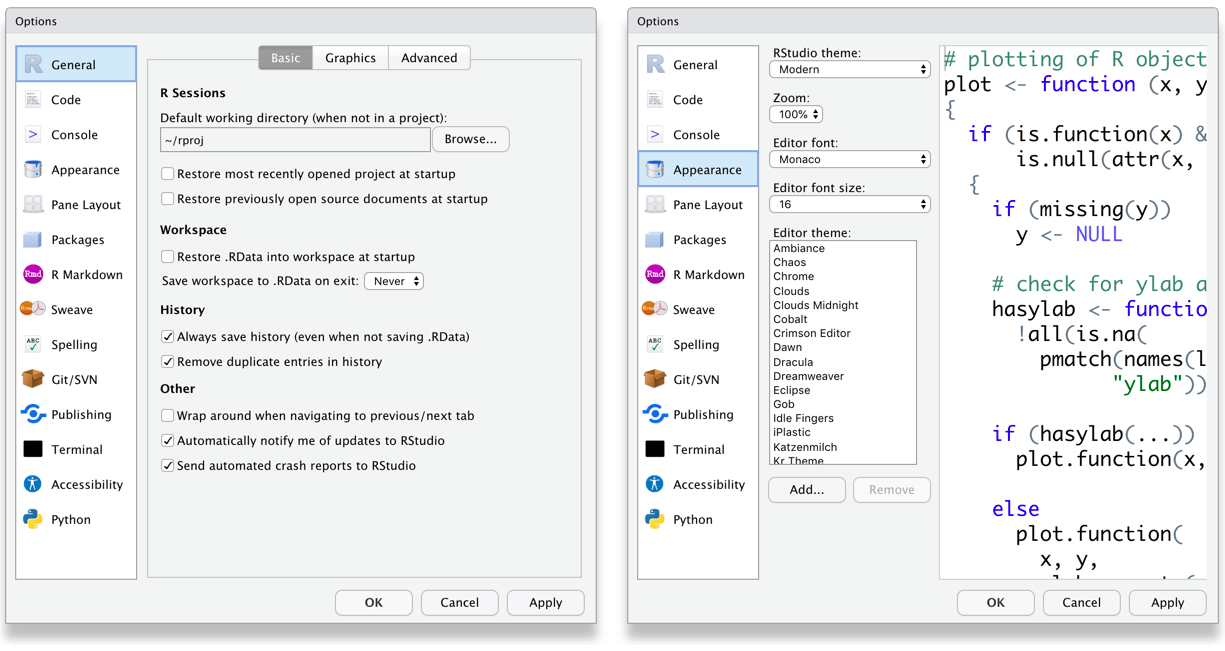
\includegraphics[width=1\linewidth]{images/rstudio_settings_general_appearance} 

}

\caption{RStudio General and Appearance settings}\label{fig:settings-general}
\end{figure}

You may also want to change the settings in the Code tab. Foe example, Lisa prefers two spaces instead of tabs for my code and likes to be able to see the whitespace{} characters. But these are all a matter of personal preference.

\begin{figure}

{\centering 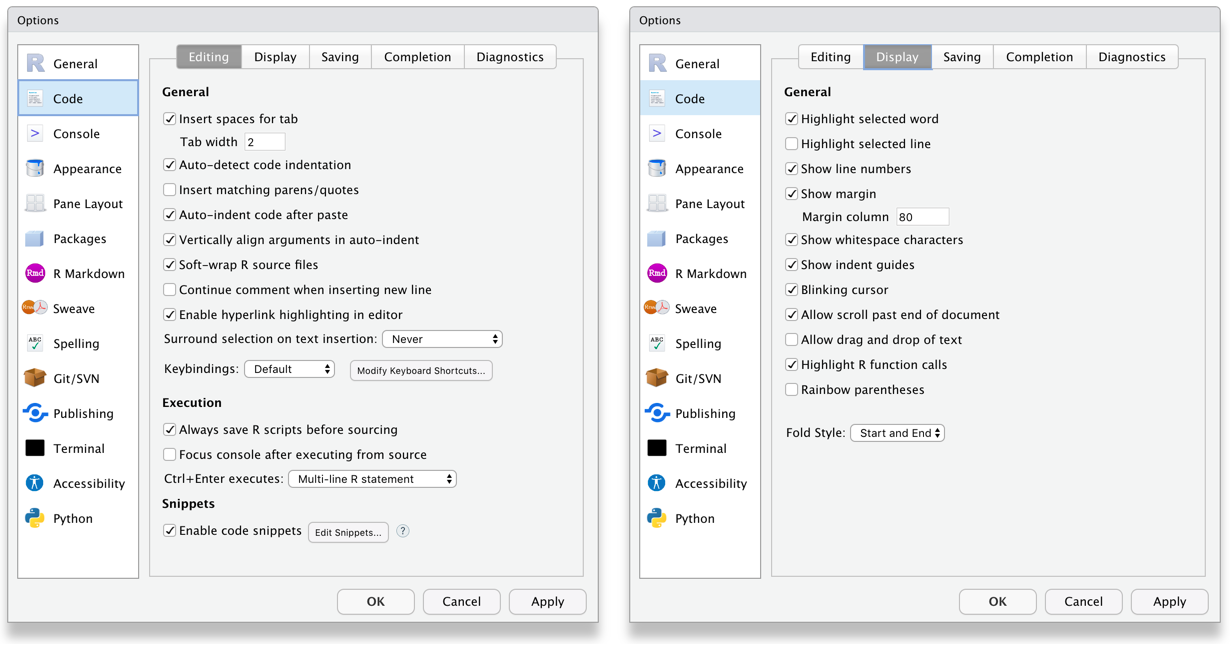
\includegraphics[width=1\linewidth]{images/rstudio_settings_code} 

}

\caption{RStudio Code settings}\label{fig:settings-code}
\end{figure}

\hypertarget{installing-latex}{%
\section{Installing LaTeX}\label{installing-latex}}

You can install the LaTeX typesetting system to produce PDF reports from RStudio. Without this additional installation, you will be able to produce reports in HTML but not PDF. This course will not require you to make PDFs. To generate PDF reports, you will additionally need to install tinytex \citep{R-tinytex} and run the following code:

\begin{Shaded}
\begin{Highlighting}[]
\NormalTok{tinytex}\SpecialCharTok{::}\FunctionTok{install\_tinytex}\NormalTok{()}
\end{Highlighting}
\end{Shaded}

\hypertarget{symbols}{%
\chapter{Symbols}\label{symbols}}

\begin{longtable}[]{@{}
  >{\centering\arraybackslash}p{(\columnwidth - 4\tabcolsep) * \real{0.1739}}
  >{\raggedright\arraybackslash}p{(\columnwidth - 4\tabcolsep) * \real{0.4130}}
  >{\raggedright\arraybackslash}p{(\columnwidth - 4\tabcolsep) * \real{0.4130}}@{}}
\toprule\noalign{}
\begin{minipage}[b]{\linewidth}\centering
Symbol
\end{minipage} & \begin{minipage}[b]{\linewidth}\raggedright
psyTeachR Term
\end{minipage} & \begin{minipage}[b]{\linewidth}\raggedright
Also Known As
\end{minipage} \\
\midrule\noalign{}
\endhead
\bottomrule\noalign{}
\endlastfoot
() & (round) brackets & parentheses \\
{[}{]} & square brackets & brackets \\
\{\} & curly brackets & squiggly brackets \\
\textless\textgreater{} & chevrons & angled brackets / guillemets \\
\textless{} & less than & \\
\textgreater{} & greater than & \\
\& & ampersand & ``and'' symbol \\
\# & hash & pound / octothorpe \\
/ & slash & forward slash \\
\textbackslash{} & backslash & \\
- & dash & hyphen / minus \\
\_ & underscore & \\
* & asterisk & star \\
\^{} & caret & power symbol \\
\textasciitilde{} & tilde & twiddle / squiggle \\
= & equal sign & \\
== & double equal sign & \\
. & full stop & period / point \\
! & exclamation mark & bang / not \\
? & question mark & \\
' & single quote & quote / apostrophe \\
'' & double quote & quote \\
\%\textgreater\% & pipe & magrittr pipe \\
\textbar{} & vertical bar & pipe \\
, & comma & \\
; & semi-colon & \\
: & colon & \\
@ & ``at'' symbol & \href{https://www.theguardian.com/notesandqueries/query/0,5753,-1773,00.html}{various hilarious regional terms} \\
\ldots{} & \texttt{glossary("ellipsis")} & dots \\
\end{longtable}

\begin{figure}

{\centering 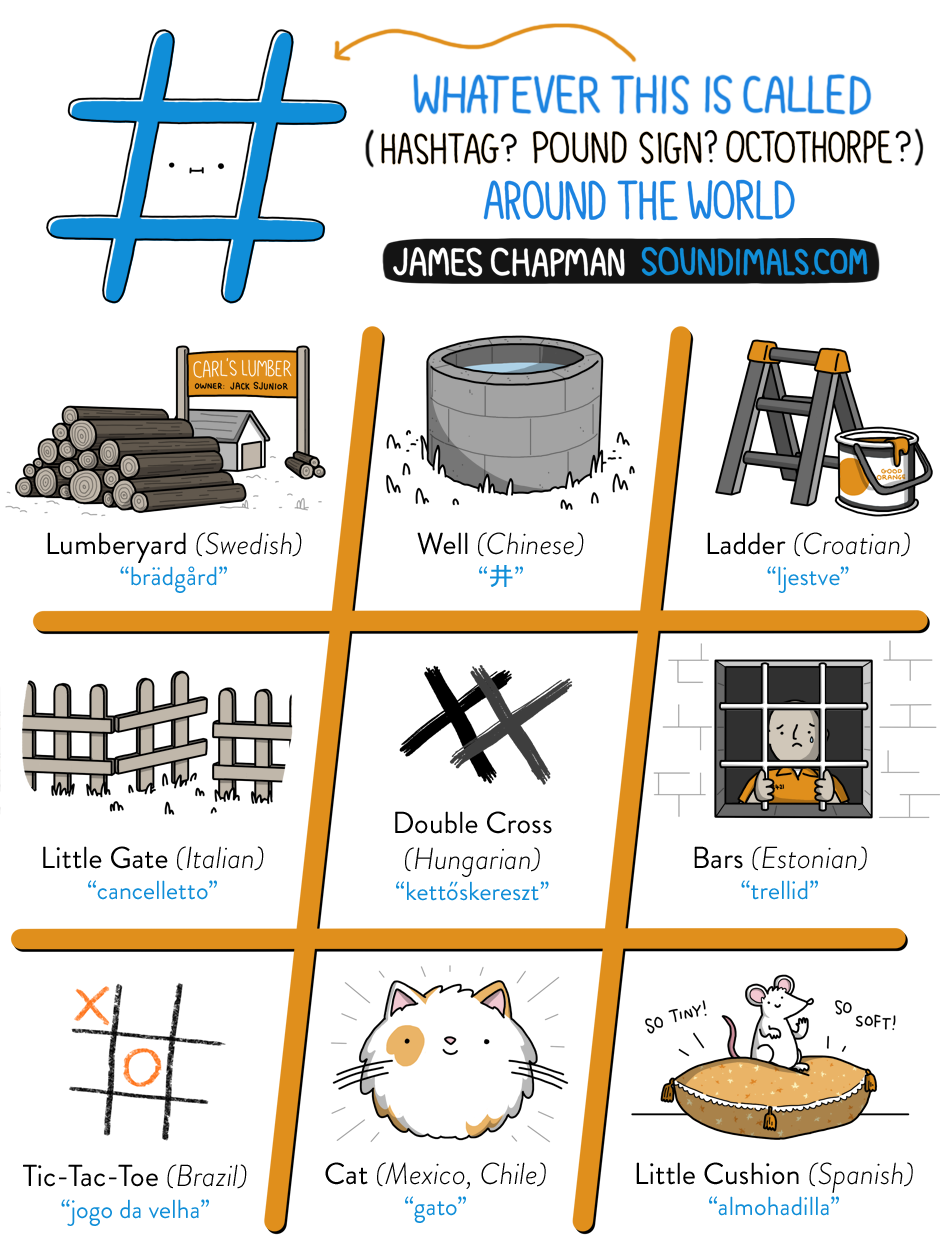
\includegraphics[width=1\linewidth]{images/soundimals_hash} 

}

\caption{[Image by James Chapman/Soundimals](https://soundimals.tumblr.com/post/167354564886/chapmangamo-the-symbol-has-too-many-names)}\label{fig:img-soundimals-hash}
\end{figure}

\hypertarget{conventions}{%
\chapter{Conventions}\label{conventions}}

This book will use the following conventions:

\begin{itemize}
\tightlist
\item
  Generic code: \texttt{list(number\ =\ 1,\ letter\ =\ "A")}
\item
  Highlighted code: {{dplyr}{::}{slice\_max}{(}{)}}
\item
  File paths: data/sales.csv
\item
  R Packages: tidyverse
\item
  Functions: {{paste}{(}{)}}
\item
  Strings: {{``psyTeachR''}}
\item
  Numbers: {{100}}, {{3.14}}
\item
  Logical values: {{TRUE}}, {{FALSE}}
\item
  Glossary items: ordinal{}
\item
  Citations: \citet{R-tidyverse}
\item
  Internal links: Chapter~\ref{inclusion}
\item
  External links: \href{https://r4ds.had.co.nz/}{R for Data Science}
\item
  Menu/interface options: \textbf{\texttt{New\ File...}}
\end{itemize}

\hypertarget{webexercises}{%
\section{Webexercises}\label{webexercises}}

See \href{https://psyteachr.github.io/webexercises/}{webexercises} for more details about how to use this in your materials.

\begin{itemize}
\item
  Type an integer: \_
\item
  I am going to learn a lot:
\item
  \begin{enumerate}
  \def\labelenumi{(\Alph{enumi})}
  \tightlist
  \item
    TRUE\\
  \end{enumerate}
\item
  \begin{enumerate}
  \def\labelenumi{(\Alph{enumi})}
  \setcounter{enumi}{1}
  \tightlist
  \item
    FALSE
  \end{enumerate}
\item
  What is a p-value?
\item
  \begin{enumerate}
  \def\labelenumi{(\Alph{enumi})}
  \tightlist
  \item
    the probability that the null hypothesis is true\\
  \end{enumerate}
\item
  \begin{enumerate}
  \def\labelenumi{(\Alph{enumi})}
  \setcounter{enumi}{1}
  \tightlist
  \item
    the probability of the observed (or more extreme) data, under the assumption that the null-hypothesis is true\\
  \end{enumerate}
\item
  \begin{enumerate}
  \def\labelenumi{(\Alph{enumi})}
  \setcounter{enumi}{2}
  \tightlist
  \item
    the probability of making an error in your conclusion
  \end{enumerate}
\end{itemize}

Hidden Text

You found some hidden text!

Hidden Code

\begin{Shaded}
\begin{Highlighting}[]
\FunctionTok{print}\NormalTok{(}\StringTok{"You found some hidden code!"}\NormalTok{)}
\end{Highlighting}
\end{Shaded}

\begin{verbatim}
## [1] "You found some hidden code!"
\end{verbatim}

\hypertarget{alert-boxes}{%
\section{Alert boxes}\label{alert-boxes}}

\begin{info}
Informational asides.

\end{info}

\begin{warning}
Notes to warn you about something.

\end{warning}

\begin{dangerous}
Notes about things that could cause serious errors.

\end{dangerous}

\begin{try}
Try it yourself.

\end{try}

\hypertarget{code-chunks}{%
\section{Code Chunks}\label{code-chunks}}

\begin{Shaded}
\begin{Highlighting}[]
\CommentTok{\# code chunks}
\FunctionTok{paste}\NormalTok{(}\StringTok{"Applied"}\NormalTok{, }\StringTok{"Data"}\NormalTok{, }\StringTok{"Skills"}\NormalTok{, }\DecValTok{1}\NormalTok{, }\AttributeTok{sep =} \StringTok{" "}\NormalTok{)}
\end{Highlighting}
\end{Shaded}

\begin{verbatim}
## [1] "Applied Data Skills 1"
\end{verbatim}

\begin{Shaded}
\begin{Highlighting}[]
\CommentTok{\# code chunks with visible r headers}
\FunctionTok{library}\NormalTok{(tidyverse)}
\end{Highlighting}
\end{Shaded}

\hypertarget{glossary}{%
\section{Glossary}\label{glossary}}

\begin{table}
\centering
\begin{tabular}{l|l}
\hline
term & definition\\
\hline
ordinal & \\
\hline
\end{tabular}
\end{table}

\hypertarget{glossary-1}{%
\chapter{Glossary}\label{glossary-1}}

You can use the \texttt{glossary()} function to automatically link to a term in the \href{https://psyteachr.github.io/glossary/}{psyTeachR glossary} or make your own project-specific glossary.

This will create a link to the glossary and include a tooltip with a short definition when you hover over the term. Use the following syntax in inline r: \texttt{glossary("word")}. For example, common data types{} are integer{}, double{}, and character{}.

If you need to link to a definition, but are using a different form of the word, add the display version as the second argument (\texttt{display}). You can also override the automatic short definition by providing your own in the third argument (\texttt{def}). Add the argument \texttt{link\ =\ FALSE} if you just want the hover definition and not a link to the psyTeachR glossary.

\begin{Shaded}
\begin{Highlighting}[]
\CommentTok{\# glossary("data type", }
\CommentTok{\#          display = "Data Types", }
\CommentTok{\#          def = "My custom definition of data types", }
\CommentTok{\#          link = FALSE)}
\end{Highlighting}
\end{Shaded}

You can add a glossary table to the end of a chapter with the following code. It creates a table of all terms used in that chapter previous to the \texttt{glossary\_table()} function. It uses \texttt{kableExtra()}, so if you use it in a code chunk, set \texttt{results=\textquotesingle{}asis\textquotesingle{}}.

\begin{Shaded}
\begin{Highlighting}[]
\FunctionTok{glossary\_table}\NormalTok{()}
\end{Highlighting}
\end{Shaded}

\begin{table}
\centering
\begin{tabular}{l|l}
\hline
term & definition\\
\hline
character & \\
\hline
data type & \\
\hline
double & \\
\hline
integer & \\
\hline
\end{tabular}
\end{table}

If you want to contribute to the glossary, fork the \href{https://github.com/PsyTeachR/glossary}{github project}, add your terms and submit a pull request, or suggest a new term at the \href{https://github.com/PsyTeachR/glossary/issues}{issues page}.

\hypertarget{license}{%
\chapter*{License}\label{license}}
\addcontentsline{toc}{chapter}{License}

This book is licensed under Creative Commons Attribution-ShareAlike 4.0 International License \href{https://creativecommons.org/licenses/by-sa/4.0/}{(CC-BY-SA 4.0)}. You are free to share and adapt this book. You must give appropriate credit \citep{psyteachr-template}, provide a link to the license, and indicate if changes were made. If you adapt the material, you must distribute your contributions under the same license as the original.

  \bibliography{book.bib,packages.bib}

\end{document}
